% Plantilla realizada por Alberto Brunete (UPM).

%parametros de tipo libro
\documentclass[10pt,a4paper]{book}

%idioma español y acentos
\usepackage[spanish, es-tabla]{babel}
%\usepackage[latin1]{inputenc}
\usepackage[utf8]{inputenc}

%algunos sÌmbolos matem·ticos y paquete para usar subim·genes
\usepackage{amsfonts}
\usepackage{graphicx}
\usepackage{subfigure}
\usepackage{listings}
\usepackage{appendix}
%M·rgenes
\usepackage[left=3cm,top=3cm,right=3cm,bottom=3cm]{geometry}

%
\usepackage{multicol}
\usepackage{pgfplots}
\pgfplotsset{compat=newest}
\usepackage{float} 
\usepackage{circuitikz}
\usepackage{tikz}
\usetikzlibrary{babel}
\usepackage{amsmath}
\usepackage{amssymb}
%para generar índice con hipervínculos
\usepackage{hyperref}
\usepackage{mathtools}
\usepackage{siunitx}
\usepackage{esint}
\usepackage{adjustbox}
\usepackage{algorithm}
\usepackage{algpseudocode}
\usetikzlibrary{tikzmark,calc}
\usepackage[acronym,nomain]{glossaries}
\floatname{algorithm}{Algoritmo}
%parametros del documento (sus propiedades)
\hypersetup{
    pdftitle={Bogurad Barañski Barañska - TFG - 2025},
    pdfsubject={TFG - año},
    pdfauthor={Bogurad Barañski Barañska},
    pdfkeywords={encriptación} {comunicaciones} {lazo de control},
    colorlinks,
    citecolor=black,
    filecolor=black,
    linkcolor=black,
    urlcolor=black,
}

%indice de gloarios 
\makeglossaries
\newtheorem{theorem}{Teorema}
\newtheorem{proof}{Demostración}

% profundidad de numeracion
\setcounter{secnumdepth}{3}
% profundidad de tabla de contenidos
\setcounter{tocdepth}{4}

\newacronym{ntt}{NTT}{Transformada Teórica de Números}
\newacronym{dft}{DFT}{Transformada Discreta de Fourier}
\newacronym{lwe}{LWE}{Aprendizaje Con Errores}
\newacronym{rlwe}{R-LWE}{Aprendizaje Con Errores en Anillos}
\newacronym{mlwe}{M-LWE}{Aprendizaje Con Errores Modular}
\newacronym{cca2}{IND-CCA2}{Indistinguibilidad bajo ataque de texto cifrado adaptable}
\newacronym{ecc}{ECC}{Criptografía en Curvas Elípticas}
\newacronym{rsa}{RSA}{Rivest-Shamir-Adleman}
\newacronym{tfo}{TFO}{Transformadas Fujisaki-Okamoto}
%empieza el documento
\begin{document}  
	\glsunsetall
	
	%elementos antes del trabajo en sÌ se meten dentro de frontmatter
	\frontmatter
	
	%cada incluye referencia a un archivo de tipo .tex
	\begin{titlepage}
\begin{center}

%forma de introducir imágenes. el \\[0.5 cm] de final de línea introduce un salto de ese tamaño.
%width=1\textwidth indica el tamaño de la imágen (valores entre 0-1). 
 
\includegraphics[width=1\textwidth]{figuras/cabecera.png}  \\[0.5 cm]

\LARGE UNIVERSIDAD POLITÉCNICA DE MADRID \\ [1 cm]

\LARGE ESCUELA TÉCNICA SUPERIOR DE INGENIERÍA Y DISEÑO INDUSTRIAL \\ [1 cm]

\LARGE Grado en Ingeniería Electrónica Industrial y Automática\\ [1 cm]

\LARGE \textbf{TRABAJO FIN DE GRADO}\\[1 cm]

\Huge \textsc{Estudio comparativo de diferentes algoritmos de encriptación para comunicaciones industriales}\\[1 cm]

\LARGE Bogurad Barañski Barañska \\[1.5 cm]

%flushleft alinea a la izquierda el texto

\begin{multicols}{2} 
\begin{flushleft} \large	
\emph{Cotutor:} Basil Mohammed Al-Hadithi\\
\emph{Departamento:} ingeniería eléctrica, electrónica, automática y física aplicada.
\end{flushleft}

\begin{flushright} \large	
\emph{Tutor:}  Roberto Gonzalez Herranz\\
\emph{Departamento:} ingeniería eléctrica, electrónica, automática y física aplicada.
\end{flushright}

\end{multicols} 

%rellena de blanco el resto de la página para escribir abajo del todo
\vfill

% Bottom of the page
{\large Madrid, Septiembre, 2025}

%SE ponen al final firmas.tex
%\end{center}
%\end{titlepage}


\cleardoublepage 
	
	%\begin{center}
% Está puesto en portada.tex
\thispagestyle{empty}
%forma de introducir imágenes. el \\[0.5 cm] de final de línea introduce un salto de ese tamaño.
%width=1\textwidth indica el tamaño de la imágen (valores entre 0-1). 

\includegraphics[width=1\textwidth]{figuras/cabecera.png}  \\[0.5 cm]

\LARGE UNIVERSIDAD POLITÉCNICA DE MADRID \\ [1 cm]

\LARGE ESCUELA TÉCNICA SUPERIOR DE INGENIERÍA Y DISEÑO INDUSTRIAL \\ [1 cm]

\LARGE Grado en Ingeniería Electrónica Industrial y Automática\\ [1 cm]

\LARGE \textbf{TRABAJO FIN DE GRADO}\\[1 cm]

\Huge \textsc{Título del trabajo}\\[4 cm]

\Large Firma Autor \\[3 cm]

%flushleft alinea a la izquierda el texto

%\begin{multicols}{2} 
%\begin{flushleft} 
%\Large \emph{Firma Cotutor (si lo hay)}
%\end{flushleft}

\begin{center} 
\Large \emph{Firma Tutor}
\end{center}

%\end{multicols} 

%rellena de blanco el resto de la página para escribir abajo del todo
\vfill

\end{center}
\end{titlepage}


\cleardoublepage 
	
	%Licencia opcional
	\begin{flushleft}

Copyright \copyright  2025. Bogurad Barañski Barañska

%ejemplo de licencia, se puede elegir cualquier otra

Esta obra está licenciada bajo la licencia Creative Commons Atribución-NoComercial-SinDerivadas 3.0 Unported (CC BY-NC-ND 3.0). Para ver una copia de esta licencia, visite http://creativecommons.org/licenses/by-nc-nd/3.0/deed.es o envíe una carta a Creative Commons, 444 Castro Street, Suite 900, Mountain View, California, 94041, EE.UU.

Todas las opiniones aquí expresadas son del autor, y no reflejan necesariamente las opiniones
de la Universidad Politécnica de Madrid.

\end{flushleft}
	
	\cleardoublepage

\begin{flushleft} \large
\textbf{Título:} Estudio comparativo de diferentes algoritmos de encriptación para comunicaciones industriales \\
\textbf{Autor:} Bogurad Barañski Barañska\\
\textbf{Tutor:} Roberto Gonzalez Herranz \\ [1 cm]

\end{flushleft} 

\begin{center} \LARGE
EL TRIBUNAL \\ [1 cm]
\end{center}

\begin{flushleft} \LARGE
Presidente: \\ [1 cm]
Vocal: \\ [1 cm]
Secretario: \\ [1.5 cm]
\end{flushleft}

\large
Realizado el acto de defensa y lectura del Trabajo Fin de Grado el día ....... de ....................   de ... en .........., en la Escuela Técnica Superior de Ingeniería y Diseño Industrial de la Universidad Politécnica de Madrid, acuerda otorgarle la CALIFICACIÓN de: \\ [2 cm]

\begin{center}
 \large VOCAL \\ [2.2 cm]
\end{center}

\begin{minipage}{0.5\textwidth}
 \begin{flushleft}
 \large SECRETARIO
\end{flushleft}
\end{minipage}
\begin{minipage}{0.5\textwidth}
\begin{flushright}
 \large PRESIDENTE
\end{flushright} 
\end{minipage}
	\chapter{Agradecimientos}

Agradezco a ............
	%chapter introduce un nuevo capítulo
\chapter{Resumen}

Este proyecto se resume en.................

\paragraph{Palabras clave:} palabraclave1, palabraclave2, palabraclave3.

\chapter{Abstract}

In this project...

\paragraph{Keywords:} keyword1, keyword2, keyword3.
	
	%genera índice
	\tableofcontents
	\addcontentsline{toc}{chapter}{Índice}
	
	%Índice de figuras.
	\listoffigures
	
	%Índice de tablas.
	\listoftables
	
	%Glosario
	\setglossarystyle{super}
	\printglossary[type=\acronymtype]


	
	
	%Empieza la parte descriptiva del trabajo
	\mainmatter
	
	\chapter{Introducción}

\section{Motivación del proyecto}
Cuando en una instalación industrial se actúa o se mide un proceso, el autómata que envía las señales puede estar situado a gran distancia de dicho proceso. Por esta razón, las comunicaciones industriales precisan el uso de buses de longitudes considerables o realizar comunicaciones a distancia. 
\newline

Aunque las comunicaciones a distancia pudieran parecer una solución más económica de implementar, tienen el problema de ser vulnerables a ataques de intermediario (alguien ajeno al proceso intercepta los mensajes enviados), lo cual pone en peligro la confidencialidad de la información. Por esta misma razón, en este trabajo se estudiarán distintos algoritmos propuestos para la encriptación de los mensajes.
\section{Objetivos}
Para realizar el proyecto, se proponen los siguientes objetivos:
\begin{itemize}
\item Implementar los siguientes algoritmos en C/C++
\begin{itemize}
	\item RSA
	\item Curvas elípticas
	\item AES 256
	\item Celosías
	\item Algoritmo de Shore
	\item Algoritmos post-cuánticos
\end{itemize}
\item Estudiar la eficacia de cifrado
\begin{itemize}
	\item Estudiar velocidad de ejecución del algoritmo
	\item Estudiar recursos requeridos por el microprocesador
	\item Estudiar la robustez del cifrado
	\item Estudiar la posibilidad de ataques de canal lateral
\end{itemize}
\item Posibilidad de ejecución en sistemas basados en FPGAs

\item Qué y cómo medir en las ECC
Intercambio de claves pública privado mediante RSA/ leif-haunman
\begin{itemize}
	\item Capacidad de memoria 
	\item Tiempo de CPU  
	\item Estudio de entropía 
\end{itemize}
\end{itemize}


\section{Herramientas utilizadas}
\subsection{LaTex \cite{latex}} 
Se ha preferido el uso de \LaTeX\ debido a la facilidad que ofrece para el maquetado de textos, superando a otras herramientas de elaboración de documentos. Además, \LaTeX\ permite crear figuras vectorizadas, representar correctamente ecuaciones y ubicar adecuadamente figuras, tablas y bibliografía.
\subsection{TikzMaker \cite{tikzmaker}} 
Esta herramienta permite crear figuras vectorizadas de \LaTeX\ mediante el paquete de circuitikz. Su principal ventaja radica en la interfaz gráfica que proporciona y en la facilidad para elaborar figuras.

\subsection{C y C++ }

\subsection{Microprocesador CY8CPROTO-063-BLE}

\section{Estructura del documento}
A continuación y para facilitar la lectura del documento, se detalla el contenido de cada capítulo:

\begin{itemize}
	\item En el capítulo 1 se realiza una introducción.
	\item En el capítulo 2 se hace un repaso de desarrollos anteriores .
	\item En el capítulo 3 se desarrollan los fundamentos matemáticos del proyecto.
	\item En el capítulo 4 se describe la implementación de los algoritmos.
	\item En el capítulo 5 se exponen los resultados obtenidos en el capítulo anterior. 
	\item En el capítulo 6 se comparan los resultados de los distintos algoritmos.
\end{itemize}
	
	%partes finales del trabajo: conclusiones, bibliografia y anexos
	
	\chapter{Estado del arte}
Los artículos que de momento tengo que son relevantes mencionar, lo haré después de los fundamentos:
\cite{NIST_IR_8413_2022} \cite{NIST_IR_8545_2025} \cite{011318_1_5.0179566} \cite{s11042-024-20535-x} \cite{A_COMPARATIVE_REVIEW_OF_DATA_ENCRYPTION_METHODS_IN_THE_USA_AND_EUROPE} \cite{An_Overview_and_Analysis_of_Hybrid_Encryption_The_Combination_of_Symmetric_Encryption_and_Asymmetric_Encryption} \cite{Comparative_Analysis_of_Energy_Costs_of_Asymmetric_vs_Symmetric_Encryption-Based_Security_Applications} \cite{First-Order-Masked-Kyber-on-ARM Cortex-M4} \cite{2022-414} \cite{An_overview_of_Quantum_Cryptography_and} \cite{2502.12252v1} \cite{Quantum_Resistance_Saber-Based_Group_Key_Exchange_Protocol_for_IoT} \cite{NISTFIPS203}
\section{Introducción}
a
\subsection{Tipos de cifrado}
a
\subsection{Necesidad del cifrado asimétrico}
a
\section{Sistemas de intercambio de claves}
a
\section{Cambio en el paradigma de cifrado asimétrico. Algoritmo de Shore}
a
\subsection{Algoritmo de Shore}
Generico: \cite{9508027v2} ECC: \cite{0301141v2} RSA: \cite{RESERCHFINAL}
\section{Evolución de los algoritmos postcuánticos}
a
\section{Cifrado asimétrico postcuántico en sistemas embebidos}
a
	
	\chapter{Fundamentos generales}
En este capítulo se desarrollan las bases matemáticas de los distintos algoritmos a implementar.
\section{Introducción}
Los algoritmos de cifrado asimétrico analizados en este Trabajo Fin de Grado corresponden a mecanismos de intercambio de claves (\acrshort{kem}), es decir, procedimientos diseñados para establecer un secreto compartido entre dos partes. Este secreto se utiliza posteriormente como clave en algoritmos de cifrado simétrico, con el fin de garantizar una comunicación segura, ya que este tipo de cifrado requiere que ambas partes dispongan previamente de una misma clave secreta.
\newline

Siguiendo las recomendaciones del \acrshort{nist} \cite{NIST_SP_800_227_ipd_2025}, uno de los enfoques consiste en establecer dichas claves a través de un canal público de comunicaciones. Para ello, de forma general y en el contexto de los algoritmos considerados en este trabajo, se emplea un esquema como el ilustrado en la figura \ref{fig:mainprotocol} donde Alice y Bob intercambian las claves mediante tres pasos:
\begin{enumerate}
	\item \textbf{Generación de llaves}: se generan una llave privada, que Alice debe mantener en secreto para no comprometer la seguridad del protocolo, y una llave pública, derivada de la privada, que Alice enviará a Bob.
	\item \textbf{Encapsulado}: Bob, usando valores la llave pública de Alice, genera un texto cifrado que enviará a Alice y el secreto compartido.
	\item \textbf{Decapsulado}: Alice, a partir del texto cifrado recibido y su llave privada, deriva el mismo secreto compartido que Bob.
\end{enumerate}


Por último, es importante señalar que existe un paso adicional denominado confirmación de claves, con el objetivo de verificar que ambas partes han obtenido el mismo secreto compartido. El \acrshort{nist} propone realizarlo mediante la generación y verificación de un código de autenticación de mensaje utilizando una clave derivada del secreto compartido. Sin embargo, los mecanismos específicos para llevar a cabo esta verificación quedan fuera del alcance del presente trabajo.
\newpage

\begin{figure}[H]
	\centering
	\begin{adjustbox}{width=0.8\textwidth}
	\begin{circuitikz}
			\tikzstyle{every node}=[font=\LARGE]
			\node [font=\LARGE, color={rgb,255:red,187; green,0; blue,255}] at (6.75,13.5) {Alice};
			\node [font=\LARGE, color={rgb,255:red,17; green,0; blue,255}] at (13.25,13.5) {Bob};
			\draw [ color={rgb,255:red,187; green,0; blue,255} ] (4.25,13) rectangle  node {\large Generar llaves} (9.25,11.5);
			\node [font=\normalsize] at (11.5,12.5) {Llave pública (pk)};
			\draw [ color={rgb,255:red,17; green,0; blue,255} ] (10.75,11) rectangle  node {\large Encapsular} (15.75,9.5);
			\draw [short] (9.25,12.25) -- (13.25,12.25);
			\draw [->, >=Stealth] (13.25,12.25) -- (13.25,11);
			\draw [short] (13.25,9.5) -- (13.25,8.25);
			\draw [ color={rgb,255:red,187; green,0; blue,255} ] (4.25,9) rectangle  node {\large Decapsular} (9.25,7.5);
			\draw [->, >=Stealth] (13.25,8.25) -- (9.25,8.25);
			\draw [->, >=Stealth] (6.75,11.5) -- (6.75,9);
			\node [font=\normalsize] at (5.25,10.25) {Llave privada (sk)};
			\node [font=\normalsize] at (11.5,8.5) {Texto cifrado (c)};
			\draw [->, >=Stealth] (13.25,8.25) -- (13.25,6.25);
			\draw [->, >=Stealth] (6.75,7.5) -- (6.75,6.25);
			\node [font=\normalsize] at (7,6) {Secreto compartido (ss)};
			\node [font=\normalsize] at (13.5,6) {Secreto compartido (ss)};
			\end{circuitikz}
		\end{adjustbox}
		\caption{Representación del protocolo empleado en los algoritmos asimétricos para establecer una clave común o secreto compartido.}
		\label{fig:mainprotocol}
	\end{figure}
	

\section{Algoritmos de Hashing }
Las funciones de hashing son funciones utilizadas para obtener una salida determinista a partir de un mensaje de entrada. Se caracterizan porque, dada la salida, no resulta factible reconstruir el mensaje original de manera eficiente.
\newline

La familia de funciones de hashing empleada en este trabajo corresponde a \acrshort{sha}3 (Secure Hash Algorithm), definida en el estándar federal \acrshort{fips}-202 \cite{FIPS202}. Dichas funciones se fundamentan en el algoritmo \texttt{Keccak-p} \cite{Keccak}, del cual se derivan cuatro funciones de hash y dos funciones de salida extendida.

\begin{itemize}
	\item \textbf{Funciones de hash}: transforman un mensaje de entrada en una salida de longitud fija de $224$, $256$, $384$ o $512$ bits, según la variante seleccionada. El nombre del algoritmo refleja dicha longitud. $SHA3-256$ genera salidas de 256 bits.
	\item \textbf{Funciones de salida extendida}: generan salidas de longitud arbitraria a partir de un mensaje de entrada. En función de la seguridad deseada se utilizan los algoritmos $SHAKE-128$ o $SHAKE-256$.
\end{itemize}
\subsection{Algoritmo \texttt{Keccak-p}}
Cada permuta dentro del algoritmo \texttt{Keccak-p}[b,n] se especifica mediante dos parámetros: 
\begin{enumerate}
	\item \textbf{El ancho de la permuta} \(b \in\{25, 50, 100, 200, 400, 800, 1600\}\): tamaño de las cadenas a permutar.
	\item \textbf{El número de rondas} \(n_r\in \mathbb{Z}\): el número de iteraciones de una transformación interna. 
\end{enumerate}
\newpage
Además del valor de \(b\) se definen dos magnitudes auxiliares \(w=b/25\) y \(l=\log_2(b/25)\).
\subsubsection{Notación básica}
En esta sección se adopta la siguiente notación

\begin{itemize}
	\item El símbolo $||$ denota la concatenación de dos cadenas.
	\item La expresión \(0^j\) representa una cadena de \(j\) bits de ceros.
	\item La función \(\texttt{len}(P)\) indica la longitud de la cadena \(P\).
	\item La notación \(Z(j)\) corresponde al \(j\)-ésimo bit de la cadena \(Z\). 
	Por ejemplo, si \(Z = 10010\), entonces \(Z(4) = 1\).
	\item La función \(\texttt{trunc}_d(Z)\) devuelve los \(d\) primeros bits de \(Z\).
\end{itemize}

\subsubsection{Vectores de estado}
En \texttt{Keccak-p} se trabaja mediante vectores de estado de tamaño \(b\), los cuales convierten las cadenas \(S\) en una matriz \(A(x,y,z)\), donde \(x, y \in \{0,1,2,3,4\}\) y \(z\) toma valores en un rango de tamaño \(w\). Esta representación al igual que la nomenclatura se representan en las figuras \ref{fig:state} y \ref{fig:partsstate}.
\begin{figure}[h]
	\centering
	\begin{minipage}{0.48\textwidth}
		\centering
		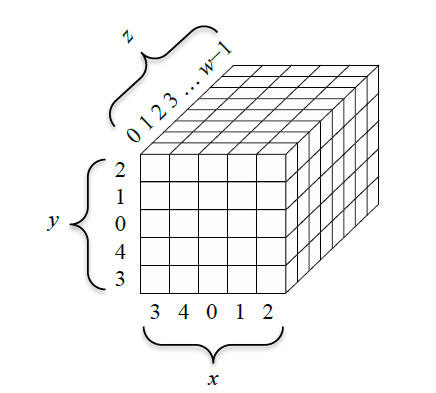
\includegraphics[width=1\linewidth]{figuras/State}
		\caption{\small Dibujo de un vector de estado \cite{FIPS202}.}
		\label{fig:state}
	\end{minipage}\hfill
	\begin{minipage}{0.51\textwidth}
		\centering
		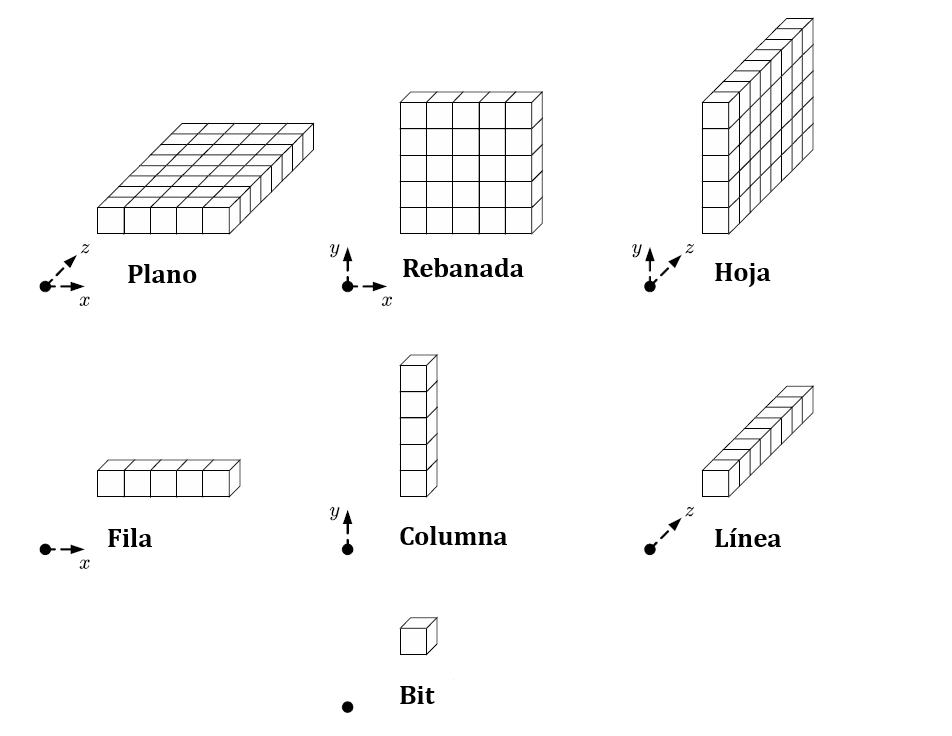
\includegraphics[width=1\linewidth]{figuras/PartsState}
		\caption{ \small Elementos de un vector de estado \cite{FIPS202}.}
		\label{fig:partsstate}
	\end{minipage}
\end{figure}

Para convertir de la cadena \(S\) en la matriz \(A\) se usa la siguiente expresión:
\begin{equation}
	A(x,y,z)=S(w\cdot(5y+x)+z)
\end{equation}

Para convertir de \(A\) a \(S\), se concatenan primero los bits dentro de cada línea, luego las líneas dentro de cada plano y, finalmente, los planos hasta formar la cadena \(S\). 
\begin{equation}
	\begin{array}{lllll}
		\text{Linea}(i,j)=&=A(i,j,0)&||A(i,j,1)&|| \hdots &|| A(i,j,w-1)\\
		\text{Plano}(j)&=\text{Linea}(0,j)&||\text{Linea}(1,j)&|| \hdots &||   \text{Linea}(4,j)\\
		S&=\text{Plano}(0)&||\text{Plano}(1)&||\hdots&|| \text{Plano}(4)
	\end{array}
\end{equation}

Una vez definidos los vectores de estado, estos se manipulan mediante cinco transformadas, denotadas \(\theta\), \(\rho\), \(\pi\), \(\chi\) y \(\iota\). Todas las transformadas toman como entrada un vector de estado \(A(x,y,z)\) y lo transforman, devolviendo un nuevo vector de estado como salida \(A'(x,y,z)\). La transformada $\iota$ recibe además como parámetro el índice de ronda \(i_r\).

\begin{enumerate}
	\item \textbf{Transformada \(\theta\)}: esta transformada realiza una XOR, $\oplus$, del bit \(A(x,y,z)\) con la paridad de las columnas \(\text{C}(x-1 \ \text{mod } 5,z)\) y $\text{C}(x+1 \ \text{mod } 5,z-1 \ \text{mod w} )$. Para ello, sigue los siguientes pasos:
	
	\begin{algorithm}[H]
		\caption{Transformada \(\theta\) en Keccak-p}
		$\begin{array}{p{\textwidth}}
			\textbf{Entrada: }\(A\) \\ 
			\hline
			\textbf{Salida: }\(A'\) \\ 
			\hline
		\end{array}$
		\begin{algorithmic}[1]
			\State Calcular la paridad de cada columna, \(C\):
			\begin{equation}
				C(x,z):=A(x,0,z) \oplus A(x,1,z) \oplus A(x,2,z) \oplus A(x,3,z) \oplus A(x,4,z) 
			\end{equation}
			\State Combinar la paridad de ambas columnas, \(D\):
			\begin{equation}
				D(x,z):=C(x-1 \bmod 5,z) \oplus C(x+1 \bmod 5,z-1 \bmod w)
			\end{equation}
			\State Realizar la XOR con el estado:
			\begin{equation}
				A'(x,y,z):=A(x,y,z)\oplus D(x,z)
			\end{equation}
			\State \Return \(A'\)
		\end{algorithmic}
	\end{algorithm}
	\item \textbf{Transformada \(\rho\)}: esta transformada rota los bits de cada línea un offset módulo la longitud de la línea. Los offsets antes de efectuar el operador módulo se listan en la tabla \ref{tab:rhooffsets}.
	
	\begin{table}[H]
		\centering
		\begin{tabular}{|c|c|c|c|c|c|}
			\hline
			& $x = 3$ & $x = 4$ & $x = 0$ & $x = 1$ & $x = 2$ \\
			\hline
			$y = 2$ & 153 & 231 & 3 & 10 & 171 \\
			\hline
			$y = 1$ & 55 & 276 & 36 & 300 & 6 \\
			\hline
			$y = 0$ & 28 & 91 & 0 & 1 & 190 \\
			\hline
			$y = 4$ & 120 & 78 & 210 & 66 & 253 \\
			\hline
			$y = 3$ & 21 & 136 & 105 & 45 & 15 \\
			\hline
		\end{tabular}
		\caption{Offsets de la transformada $\rho$.}
		\label{tab:rhooffsets}
	\end{table}
	
	Para realizar estas rotaciones sigue los siguientes pasos:
	\begin{algorithm}[H]
		\caption{Transformada \(\rho\) en Keccak-p}
		$\begin{array}{p{\textwidth}}
			\textbf{Entrada: }\(A\) \\ 
			\hline
			\textbf{Salida: }\(A'\) \\ 
			\hline
		\end{array}$
		\begin{algorithmic}[1]
			\State Asignar el caso especial de \((x,y,z):=(0,0,z)\):
			\begin{equation}
				A'(0,0,z):=A(0,0,z)
			\end{equation}
			\For{\(t=0:23\)} \Comment{Para los \(23\) valores restantes}
			\State Asignar el valor de la tabla \ref{tab:rhooffsets} modulo \(w\) a cada punto:
			\begin{equation}
				A'(x,y,z):=A(x,y,[z-(t+1)(t+2)/2 \ \text{mod w}])
			\end{equation}
			\State Asignar \((x,y):=(y,2x+3y \ \text{mod } 5)\)
			\EndFor
			\State \Return \(A'\)
		\end{algorithmic}
	\end{algorithm}
	\newpage
	\item \textbf{Transformada \(\pi\)}: esta transformada rota las coordenadas de cada rebanada \((x,y)\) tal como se ilustra en la tabla \ref{tab:piTransform}.
	
	\begin{table}[H]
		\centering
		\begin{tabular}{|c|c|c|c|c|c|}
					\hline
			& $x = 3$ & $x = 4$ & $x = 0$ & $x = 1$ & $x = 2$ \\
			\hline
			$y = 2$ & (4,3) & (0,4) & (1,0) & (2,1) & (3,2) \\
			\hline
			$y = 1$ & (1,3) & (2,4) & (3,0) & (4,1) & (0,2) \\
			\hline
			$y = 0$ & (3,3) & (4,4) & (0,0) & (1,1) & (2,2) \\
			\hline
			$y = 4$ & (0,3) & (1,4) & (2,0) & (3,1) & (4,2) \\
			\hline
			$y = 3$ & (2,3) & (3,4) & (4,0) & (0,1) & (1,2) \\
			\hline
		\end{tabular}
		\caption{Tabla de transformación $\pi$. Para obtener el valor de $A'(x,y)$, se debe leer el valor de la posición $(x',y')$ indicada en la celda correspondiente de la matriz original $A$.}
		\label{tab:piTransform}
	\end{table}
	
	Para realizar esta rotación se sigue el siguiente algoritmo:
	\begin{algorithm}[H]
		\caption{Transformada \(\pi\) en Keccak-p}
		$\begin{array}{p{\textwidth}}
			\textbf{Entrada: }\(A\) \\ 
			\hline
			\textbf{Salida: }\(A'\) \\ 
			\hline
		\end{array}$
		\begin{algorithmic}[1]
			\State Calcular la rotación:
			\begin{equation}
				A'(x,y,z):=A(x+3y \ \text{mod } 5,x,z)
			\end{equation}
			\State \Return \(A'\)
		\end{algorithmic}
	\end{algorithm}
	
	
	\item \textbf{Transformada \(\chi\)}: esta transformada actualiza cada bit como el XOR entre el bit original y una combinación no lineal de sus vecinos en la misma fila mediante una puerta AND como se puede ver en la figura \ref{fig:chitransform}.
	
	\begin{figure}[H]
		\centering
		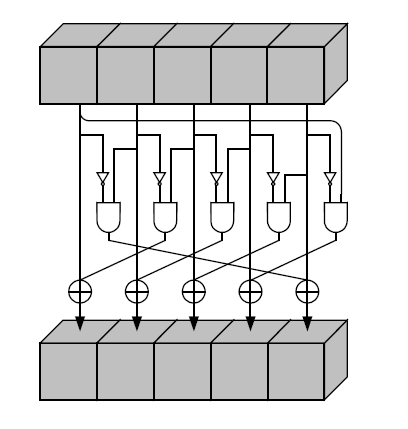
\includegraphics[width=0.4\linewidth]{figuras/PartsState1}
		\caption{Representación de la transformada $\chi$ realizada en cada fila \cite{FIPS202}. Arriba la matriz \(A(x,y,z)\) y abajo la matriz \(A'(x,y,z)\).}
		\label{fig:chitransform}
	\end{figure}
	\newpage
	Para realizar esta rotación se sigue el siguiente algoritmo:
	\begin{algorithm}[H]
		\caption{Transformada \(\chi\) en Keccak-p}
		$\begin{array}{p{\textwidth}}
			\textbf{Entrada: }\(A\) \\ 
			\hline
			\textbf{Salida: }\(A'\) \\ 
			\hline
		\end{array}$
		\begin{algorithmic}[1]
			\State Calcular la rotación:
			\begin{equation}
				A'(x,y,z):=A(x,y,z)\oplus\{[A(x+1 \ \text{mod } 5 ,y,z)\oplus 1]\& A(x+2 \ \text{mod } 5 ,y,z)\}
			\end{equation}
			\State \Return \(A'\)
		\end{algorithmic}
	\end{algorithm}
	
	\item \textbf{Transformada \(\iota\)}: esta transformada modifica solo algunos bits de la línea \((0,0)\) de tal manera que que dependa del índice de ronda \(i_r\). Para ello, se sigue el siguiente algoritmo:
	\begin{algorithm}[H]
		\caption{Transformada \(\iota\) en Keccak-p}
		$\begin{array}{p{\textwidth}}
			\textbf{Entrada: }\(A\), \(i_r\) \\ 
			\hline
			\textbf{Salida: }\(A'\) \\ 
			\hline
		\end{array}$
		\begin{algorithmic}[1]
			\State Asignar:
			\begin{equation}
				A'(x,y,z):=A(x,y,z)
			\end{equation}
			\State Inicializar el vector de ceros \(RC\) de longitud \(w\):
			\For{j=0:l} \Comment{\(l=\log_2(b/25)\) }
			\State Asignar
			\begin{equation}
				RC(2^j-1):=\texttt{rc}(j+7i_r)
			\end{equation}
			\EndFor
			\State Asignar:
			\begin{equation}
				A'(0,0,z):=A'(0,0,z)\oplus RC(z)
			\end{equation} 
			
			\State \Return \(A'\)
		\end{algorithmic}
	\end{algorithm}
	 
	Este algoritmo depende de la función \(\texttt{rc}(t)\)la cual, dado un entero, $t$, genera un bit mediante un procedimiento basado en un registro de desplazamiento con retroalimentación lineal como se describe en el siguiente algoritmo:
	\begin{algorithm}[H]
		\caption{rc}
		$\begin{array}{p{\textwidth}}
			\textbf{Entrada: }\(t\)\\ 
			\hline
			\textbf{Salida: }\(rc(t)\) \\ 
			\hline
		\end{array}$
		\begin{algorithmic}[1]
			\If{\(t \ \text{mod } 255 =0\)}
			\State \Return 1
			\EndIf
			\For{i=1:t mod \(255\)}
			\State \(R:=R||R\)
			\State \(R[0]:=R[0]\oplus R[8]\)
			\State \(R[4]:=R[4]\oplus R[8]\)
			\State \(R[5]:=R[5]\oplus R[8]\)
			\State \(R[6]:=R[6]\oplus R[8]\)
			\State \(R:=\texttt{Trunc}_8[R]\) 
			\EndFor
			\State \Return \(R[0]\)
		\end{algorithmic}
	\end{algorithm}
\end{enumerate}
\newpage

Una vez descritas estas transformadas la función de cada ronda, \(\texttt{Rnd}(A,i_r)\) se define como:
\begin{equation}
	\texttt{Rnd}(A,i_r)=\iota(\chi(\pi(\rho(\theta(A)))),i_r)
\end{equation}

Con esta función ya se puede describir el algoritmo \(\texttt{Keccak-p}(b,n_r)\) que consiste en ejecutar \(n_r\) iteraciones de \texttt{Rnd} para una cadena de longitud \(b\):

\begin{algorithm}[H]
\caption{Keccak-p}
$\begin{array}{p{\textwidth}}
	\textbf{Entrada: }\(S\), \(n_r\) \\ 
	\hline
	\textbf{Salida: }\(S'\)\\ 
	\hline
\end{array}$
\begin{algorithmic}[1]
	\State Convertir \(S\) en un vector de estado \(A\)
	\For{$i_r$=12+2l-$n_r$:12+2l-1}
	\State A=\texttt{Rnd}$(A,i_r)$
	\EndFor
	\State Convertir \(A\) en una cadena \(S'\) de longitud \(b\)
	\State \Return \(S'\)
\end{algorithmic}
\end{algorithm}
\subsubsection{Función esponja}
Este tipo de función, $\texttt{sponge}[f,pad,r](N,d)$, permite convertir una entrada binaria, \(N\), de cualquier longitud a una salida, \(Z\), de longitud \(d\). Para ello, usa tres componentes:
\begin{enumerate}
	\item Una función sobre cadenas de longitud fija, \(f\).
	\item Una regla de relleno, \(pad\).
	\item Un parámetro llamado velocidad, \(r\), menor que la longitud, \(b\), de las cadenas que procesa \(f\).
\end{enumerate}

La función \texttt{sponge}, ilustrada en la figura \ref{fig:esponja}, aplica la regla de relleno sobre la entrada y procesa la información mediante los tres componentes descritos. En la fase de absorción, el mensaje se divide en bloques de longitud \(r\), que se incorporan iterativamente al estado interno de longitud \(b\) utilizando la permutación \(f\), que en este caso es \texttt{keccak-p}. En esta construcción se impone que el parámetro de capacidad sea
\begin{equation}
	c = b - r
\end{equation}

Tras finalizar la fase de absorción, se inicia la fase de extracción, en la que se producen bloques de salida de tamaño \(r\) de manera iterativa hasta obtener los \(d\) bits requeridos.
\newpage
\begin{figure}[H]
	\centering
	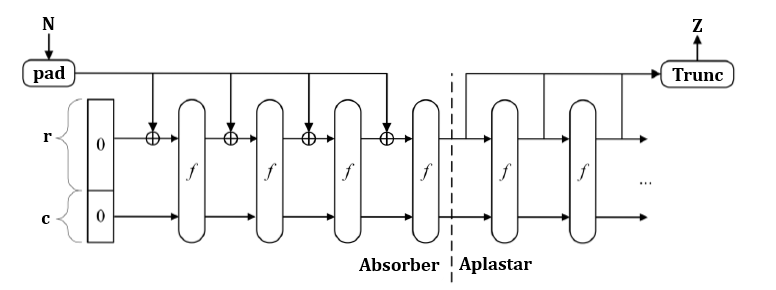
\includegraphics[width=1\linewidth]{figuras/esponja}
	\caption{Representación visual del funcionamiento del algoritmo \texttt{sponge} \cite{FIPS202}.}
	\label{fig:esponja}
\end{figure}


Teniendo en cuenta la descripción anterior la función \texttt{sponge} se define como:
\begin{algorithm}[H]
	\caption{sponge}
	$\begin{array}{p{\textwidth}}
		\textbf{Entrada: }\(N\), \(d\) \\ 
		\hline
		\textbf{Salida: }Z\\ 
		\hline
	\end{array}$
	\begin{algorithmic}[1]
		\State Calcular:
		\begin{equation}
			P=N||\texttt{pad}(r,\texttt{len}(N))
		\end{equation}
		\State Calcular:
		\begin{equation}
			n=\dfrac{len(P)}{r}
		\end{equation}
		\State Asignar \(c=b-r\) y \(S=0^b\)
		\State Sea \(P_0,\hdots , P_{n-1}\) la secuencia de cadenas de longitud \(r\) tal que \(P=P_0||\hdots ||P_{n-1}\).
		\For{i=0:n-1}
		\State Asignar:
		\begin{equation}
			S=f(S\oplus (P_i||0^c))
		\end{equation}
		\EndFor
		\State Inicializar \(Z\) como una cadena vacía
		\State Asignar 
		\begin{equation}
			Z=Z||\texttt{Trunc}_r(S)
		\end{equation}
		\If{\(d\le len(Z)\)}
		\State \Return \(\texttt{Trunc}_d(S)\)
		\EndIf
		\State Asignar: 
		\begin{equation}
			S=f(S)
		\end{equation}
		\State Ir al paso 9		
	\end{algorithmic}
\end{algorithm}

El algoritmo de relleno utilizado en la función \texttt{sponge} es el algoritmo \texttt{pad10*1} que dado un entero positivo, \(x\) y un entero no negativo \(m\) se obtiene una cadena, \(P\), de tal manera que:
 \begin{equation}
 	m+\texttt{len}(P)=\lambda x
 \end{equation}
 
El algoritmo de \texttt{pad10*1}: 
\begin{algorithm}[H]
	\caption{pad10*1}
	$\begin{array}{p{\textwidth}}
		\textbf{Entrada: }\(x\), \(m\) \\ 
		\hline
		\textbf{Salida: }P\\ 
		\hline
	\end{array}$
	\begin{algorithmic}[1]
		\State Asignar:
		\begin{equation}
			j=-m-2 \ \text{mod } x
		\end{equation}
		\State Calcular
		\begin{equation}
			P=1|| 0^j||1
		\end{equation}
		\State \Return $P$
	\end{algorithmic}
\end{algorithm}

Definida la función de esponja, para el caso de \(b=1600\) el algoritmo de la familia Keccak se denomina $\texttt{Keccak}[c](N,d)$. Este algoritmo tiene la siguiente definición:
\begin{equation}
	\texttt{Keccak}[c](N,d)=\texttt{sponge}[\texttt{Keccak-p}(1600,24),\texttt{pad10*1},1600-c](N,d)
\end{equation}


Por tanto, las funciones de hash se definen como:
\begin{enumerate}
	\item \texttt{SHA3-224}$(M)$=\texttt{Keccak}[448]$(M||01,224)$
	\item \texttt{SHA3-256}$(M)$=\texttt{Keccak}[512]$(M||01,256)$
	\item \texttt{SHA3-384}$(M)$=\texttt{Keccak}[768]$(M||01,384)$
	\item \texttt{SHA3-512}$(M)$=\texttt{Keccak}[1024]$(M||01,512)$
	\item \texttt{SHAKE128}$(M,d)$=\texttt{Keccak}[256]$(M||1111,d)$
	\item \texttt{SHAKE256}$(M,d)$=\texttt{Keccak}[512]$(M||1111,d)$
\end{enumerate}
\subsubsection{Seguridad}
Mediante la tabla 4 del artículo \cite{FIPS202} se muestra la seguridad en bits que tienen cada uno de los algoritmos \acrshort{sha}3. Estas tres condiciones de seguridad para un algoritmo de hash son las siguientes:
\begin{enumerate}
	\item \textbf{Resistencia a la colisión}: dificultad para encontrar dos entradas diferentes que producen el mismo hash. Esta propiedad previene ataques donde dos mensajes diferentes se pueden sustituir sin que se pueda detectar.
	\item \textbf{Resistencia a preimagen}: dificultad para que dado un hash, \(h\), se pueda encontrar una entrada, \(x\), tal que \(\texttt{hash}(x)=h\). Esta propiedad permite proteger datos sensibles de tal manera que si el hash se revela no comprometa las contraseñas. 
	\item \textbf{Resistencia a preimagen secundaria}: dificultad para que dada una entrada, \(x_1\), se pueda encontrar una entrada diferente, \(x_2\), que cumpla \(\texttt{hash}(x_1)=\texttt{hash}(x_2)\). Esta propiedad previene la falsificación de mensajes.
\end{enumerate}
\newpage



\section{Funcionamiento básico de los algoritmos postcuánticos}
En esta sección se describe el funcionamiento de los algoritmos postcuánticos analizados en este trabajo. Dado que no se desarrollaron implementaciones propias, sino que se utilizó el código proporcionado por el \acrshort{nist} en la tercera \cite{nistPQCround3} y cuarta \cite{nistPQCround4} ronda del proceso de estandarización, resulta apropiado presentar su funcionamiento aquí en lugar de en la sección de desarrollo.
\subsection{Fundamentos matemáticos de CRYSTALS-Kyber }
Se utilizará la misma notación empleada en el artículo \cite{kyber-spec-2021}. El conjunto de los enteros sin signo de 8 bits se denota por \(\mathcal{B} = \{0, \dots, 255\}\). Para representar vectores de tamaño \(k\), se utiliza la notación \(\mathcal{B}^k\), mientras que para vectores de tamaño arbitrario se emplea \(\mathcal{B}^*\).
\newline

Para trabajar con estos vectores, se utiliza el símbolo \(||\) para denotar la concatenación de dos cadenas, y la notación \(+k\) para indicar el desplazamiento de \(k\) bytes desde el inicio de una cadena. Por ejemplo, si se tiene una cadena \(a\) de longitud \(l\) y se concatena con una cadena \(b\), se obtiene:
\begin{equation}
	c = a || b
\end{equation}

Entonces:
\begin{equation}
	b = c + l
\end{equation}

Para denotar vectores, se utiliza la notación \(v[i]\), donde \(v\) es un vector columna e \(i\) indica la posición del elemento (empezando desde 0, si no se indica lo contrario). Para las matrices, se emplea la notación \(A[i][j]\), donde \(i\) representa la fila y \(j\) la columna. La transpuesta de una matriz \(A\) se denota como \(A^T\).
\newline

Se denota mediante \(\lfloor x \rceil\) el redondeo de \(x\) al entero más cercano. Por ejemplo: \(\lfloor 2{,}3 \rceil = 2\), \(\lfloor 2{,}5 \rceil = 3\) y \(\lfloor 2{,}8 \rceil = 3\).
\newline

Se denota mediante $\left\| x\right\|$ al valor absoluto de x.
\newline

Para las reducciones modulares se emplean dos tipos: una centrada en cero y otra correspondiente a la reducción modular estándar. Para la reducción modular centrada en cero, sea \(\alpha\) un entero par. Esta operación se define como:
\begin{equation}
	r' = r \ \text{mod}^{\pm} \alpha \quad \Longrightarrow \quad -\dfrac{\alpha}{2} < r' \le \dfrac{\alpha}{2}
\end{equation}

Mientras que la reducción modular estándar se denota como:
\begin{equation}
	r' = r \ \text{mod}^{+} \alpha \quad \Longrightarrow \quad 0 \le r' < \alpha
\end{equation}

Finalmente, se denota mediante \(s \leftarrow S\) la selección de \(s\) de manera uniformemente aleatoria del conjunto \(S\). Si \(S\) representa una distribución de probabilidad, entonces \(s\) se selecciona de acuerdo con dicha distribución.
\newpage

\subsubsection{Transformada Teórica de Números o Number Theoretic Transform (\acrshort{ntt})}
Para acelerar las operaciones de multiplicación en el esquema basado en retículas, se utiliza la Transformada Teórica de Números (\acrshort{ntt}, por sus siglas en inglés), la cual permite reducir la complejidad temporal de la multiplicación de polinomios desde \(\mathcal{O}(n^2)\), correspondiente al método tradicional, hasta \(\mathcal{O}(n \log(n))\). Para más detalles, consúltese \cite{cryptoeprint:2024/585}.
\newline

Antes de pasar a explicar el funcionamiento de este método es relevante aclarar que se trabaja sobre el siguiente anillo de polinomios para realizar las operaciones, denotado mediante \(R_q\):
\begin{equation}
	R_q \coloneqq \dfrac{\mathbb{Z}_q[X]}{X^n + 1}
\end{equation}

En la implementación especificada de Kyber, según el artículo \cite{kyber-spec-2021}, se utiliza un valor de \(q=3329\) y \(n=256\). Esta elección es esencial para permitir el uso de la multiplicación mediante la Transformada Teórica de Números (\acrshort{ntt}), la cual requiere que \(n| (q-1)\), es decir, que \(n\) divida a \((q-1)\). Esta condición garantiza la existencia de \(n\) raíces enésimas de la unidad en \(Z_q\), lo cual es necesario para definir la \acrshort{ntt}. La validez de esta afirmación se fundamenta en el siguiente teorema\protect\footnotemark[\value{footnote}]:
\newline

\begin{theorem}
	Para \(n\), \(q>1\), el cuerpo  \(Z_q\) tiene una raíz enésima de la unidad si y solo sí \(n| (q-1)\)
\end{theorem} 
\begin{proof}
	Si \(\omega\) es una raíz enésima de la unidad en el conjunto \( \mathbb{Z}_q \), entonces el conjunto:
	\begin{equation}
		\Omega = \left\{1, \omega, \omega^2, \dots, \omega^{n-1} \right\}
	\end{equation}
	forma un subgrupo cíclico \( H \) del grupo multiplicativo \( G_{q-1} \). Por el Teorema de Lagrange, se concluye que el orden de \( H \) divide al orden de \( G_{q-1} \), es decir, \( n \mid (q-1) \).
	\newline
	
	Dado que \( G_{q-1} \) es también un grupo cíclico, existe un generador \(\alpha\) tal que, por el pequeño teorema de Fermat, se cumple:
	\begin{equation}
		\alpha^{q-1} = 1
	\end{equation}
	
	Por lo tanto, el grupo \( G_{q-1} \) puede escribirse como:
	\begin{equation}
		G_{q-1} = \left\{1, \alpha, \alpha^2, \dots, \alpha^{q-2} \right\}
	\end{equation}
	
	Si se define \(\omega\) como:
	\begin{equation}
		\omega = \alpha^{\frac{q-1}{n}},
	\end{equation}
	
	entonces:
	\begin{equation}
		\omega^n = \alpha^{q-1} = 1,
	\end{equation}
	
	y además, para todo \( 0 < k < n \), se cumple:
	\begin{equation}
		k \cdot \frac{q-1}{n} < q-1 \quad \Rightarrow \quad \omega^k \neq 1.
	\end{equation}
	
	Por lo tanto, \(\omega\) es una raíz enésima de la unidad en \(\mathbb{Z}_q\).
\end{proof}
\footnotetext{
	Extraído de la siguiente página web: \url{https://www.csd.uwo.ca/~mmorenom/CS874/Lectures/Newton2Hensel.html/node9.html}
}
\newpage

Por tanto, el polinomio \(X^{256} + 1\) se puede factorizar sobre el cuerpo \(\mathbb{Z}_q\). En la implementación concreta del esquema Kyber, este polinomio se descompone en 128 factores cuadráticos.
\newline

A este polinomio se le aplica la transformada \acrshort{ntt} a sus coeficientes, la cual no es más que una variación de la \acrshort{dft} aplicada a cuerpos finitos \(\mathbb{Z}_q\) y aplicada a polinomios de grado \(n\). Para ello, se definen dos operaciones fundamentales:
\begin{enumerate}
	\item La transformada directa:
	\begin{equation}
		\hat{a}_j=\sum_{i=0}^{n-1} \phi^{i\left(2j+1\right)} a_j \ \text{mod} \ q
	\end{equation}
	\item  La transformada inversa:
	\begin{equation}
		a_i=n^{-1} \sum_{j=0}^{n-1} \phi^{-i\left(2j+1\right)} \hat{a}_j \ \text{mod} \ q
	\end{equation}
\end{enumerate}

Donde $\phi$ es un valor tal que $\phi^2=\omega$, con $\omega$ una raíz enésima de la unidad en \(\mathbb{Z}_q\) y \(n^{-1}\) es la inversa multiplicativa de \(n\) en \(\mathbb{Z}_q\).
\newline

A continuación, se presenta un ejemplo extraído de \cite{cryptoeprint:2024/585} para ilustrar su funcionamiento. Sea el polinomio \(G(x)=5+6x+7x^2+8x^3\), cuyo vector de coeficientes es \(g=[5,6,7,8]\). Trabajando en el anillo \(\mathbb{Z}_{7681}\), y tomando $\phi=1925$, se puede calcular la transformada \acrshort{ntt} \(\hat{g}\). Aplicando luego la transformada inversa, es posible recuperar el vector original \(g\).
\begin{equation}
	\hat{g}=\begin{bmatrix}
		\phi^0 & \phi^1 & \phi^2 & \phi^3\\
		\phi^0 & \phi^3 & \phi^6 & \phi^1\\
		\phi^0 & \phi^5 & \phi^2 & \phi^7\\
		\phi^0 & \phi^7 & \phi^6 & \phi^5\\
	\end{bmatrix} \cdot \begin{bmatrix}
	5\\
	6\\
	7\\
	8
	\end{bmatrix}=\begin{bmatrix}
	1 & 1925 & 3383 & 6468\\
	1 & 6468 & 4298 & 1925\\
	1 & 5756 & 3383 & 1213\\
	1 & 1213 & 4298 & 5756\\
	\end{bmatrix} \cdot \begin{bmatrix}
	5\\
	6\\
	7\\
	8 \end{bmatrix}= \begin{bmatrix}
	2489\\
	7489\\
	6478\\
	6607 \end{bmatrix}
\end{equation}

Aplicando la transformada inversa, donde la inversa de $\phi=1925$ en \(\mathbb{Z}_{7681}\) es $\phi^{-1}=1213$ y el inverso del orden del polinomio \(n=4\) es \(n^{-1}=5761\):
\begin{equation}
	g=n^{-1}\begin{bmatrix}
		\phi^0 & \phi^0 & \phi^0 & \phi^0\\
		\phi^{-1} & \phi^{-3} & \phi^{-5} & \phi^{-7}\\
		\phi^{-2} & \phi^{-6} & \phi^{-2} & \phi^{-6}\\
		\phi^{-3} & \phi^{-1} & \phi^{-7} & \phi^{-5}\\
	\end{bmatrix} \cdot \hat{g}=5761\begin{bmatrix}
	1 & 1 & 1 & 1\\
	1213& 5756& 6468& 1925\\
	4298& 3383& 4298& 3383\\
	5756& 1213& 1925& 6468\\
	\end{bmatrix} \cdot \begin{bmatrix}
	2489\\
	7489\\
	6478\\
	6607 \end{bmatrix}
\end{equation}

Con estas transformadas definidas se define el producto o convolución negativa en el anillo \(	R_q \coloneqq \dfrac{\mathbb{Z}_q[X]}{X^n + 1}\) entre dos polinomios \(g\) y \(h\) como:
\begin{equation}
	g\cdot h= \text{NTT}^{-1}(\text{NTT}(g)\circ\text{NTT}(h))
\end{equation}

Donde la operación \(\circ\) denota la multiplicación elemento a elemento (o punto a punto) entre los vectores en ${Z}_q[X]$.
\newpage

Ahora, queda demostrar que el tiempo de ejecución de la \acrshort{ntt} es de \(\mathcal{O}(n \log(n))\). Para lograr este cometido, se aprovechan dos propiedades que cumplen estas raíces calculadas:
\begin{enumerate}
	\item Peridicidad: 
	\begin{equation}
		\phi^{k+2n}=\phi^k
	\end{equation}
	\item Simetría:
	\begin{equation}
		\phi^{k+n}=\phi^{-k}
	\end{equation}
\end{enumerate}

Con estas propiedades, se puede implementar el algoritmo de Cooley-Tukey \cite{CooleyALG} que consiste en ir descomponiendo el problema en mitades de manera recursiva para reducir al máximo la cantidad de cálculos realizados. Partiendo de la transformada directa y desarrollando:
\begin{equation}
	\hat{a}_j=\sum_{i=0}^{n-1} \phi^{i\left(2j+1\right)} a_j \ \text{mod} \ q = \sum_{i=0}^{n/2-1} \phi^{4ij+2i} a_{2i} + \phi^{2j+1} \sum_{i=0}^{n/2-1} \phi^{4ij+2i} a_{2i+1} \ \text{mod} \ q
\end{equation}

Si se sustituye \(A_j=\sum_{i=0}^{n/2-1} \phi^{4ij+2i} a_{2i}\) y \(B_j=\sum_{i=0}^{n/2-1} \phi^{4ij+2i} a_{2i+1}\). Ahora aplicando simetría en \(\phi\):
\begin{equation}
	\hat{a}_j=A_j+\phi^{4ij+2i}B_j  \ \text{mod} \ q
\end{equation}
\begin{equation}
	\hat{a}_{j+n/2}=A_j-\phi^{4ij+2i}B_j  \ \text{mod} \ q
\end{equation}

Donde las matrices \(A_j\) y \(B_j\)pueden obtenerse como el resultado de aplicar la \acrshort{ntt} sobre la mitad de los puntos, gracias a la estructura recursiva del algoritmo. Esto implica que, si \(n\) es una potencia de \(2\), el proceso puede repetirse recursivamente sobre subproblemas de tamaño cada vez menor, hasta alcanzar el caso base. 
\newline

De manera similar, se puede mostrar esta propiedad para la transformada inversa. Por tanto, se demuestra que este algoritmo tiene complejidad \(\mathcal{O}(n \log(n))\).
\newline

En el caso concreto de Kyber \cite{kyber-spec-2021}, la Transformada (\acrshort{ntt}) de un polinomio en el anillo \(R_q\) se representa como un vector de 128 polinomios de grado 1.
\newline

Sean las 256 raíces enésimas de la unidad \(\left\{\xi, \xi^3, \dots, \xi^{255}\right\}\), con \(\xi = 17\) como primera raíz primitiva. Entonces, se cumple que:
\begin{equation}
	X^{256}+1=\prod_{i=0}^{127}\left(X^2- \xi^{2i+1}\right)
\end{equation}

Aplicando la \acrshort{ntt} propuesta en \cite{kyber-spec-2021} a un polinomio \(f\in R_q\) se obtiene:
\begin{equation}
	NTT(f)=\hat{f}=\left(\hat{f}_0+\hat{f}_1X,\hat{f}_2+\hat{f}_3X,...,\hat{f}_{254}+\hat{f}_{255}X\right)
\end{equation}

Con
\begin{equation}
	\begin{array}{l}
		\hat{f}_{2i}=\sum\limits_{j=0}^{127} f_{2j}\xi^{\left(2i+1\right)j}\\
		\hat{f}_{2i+1}=\sum\limits_{j=0}^{127} f_{2j+1}\xi^{\left(2i+1\right)j}
	\end{array}
\end{equation}

Donde mediante la transformada directa \acrshort{ntt} e inversa \acrshort{ntt}$^{-1}$ se puede realizar el producto de \(f\),\(g\in R_q\) de manera eficiente de la siguiente manera: 
\begin{equation}
	h=f\cdot g = \text{NTT}^{-1}\left[\text{NTT}(f) \circ \text{NTT}(g)\right]
\end{equation}

Siendo \(\hat{h}=\hat{f}\circ\hat{g}=\text{NTT}(f)\circ \text{NTT}(g)\) la multiplicación base definida como:
\begin{equation}
	\hat{h}_{2i}+\hat{h}_{2i+1}X=(\hat{f}_{2i}+\hat{f}_{2i+1})\left(\hat{g}_{2i}+\hat{g}_{2i+1}\right) \ \text{mod} \left(X^2-\xi^{2i+1}\right)
\end{equation}


En la figura \ref{fig:NTTFigure} se puede ver una representación gráfica de como funciona este proceso.
\begin{figure}[H]
	\centering
		\begin{circuitikz}
			\tikzstyle{every node}=[font=\LARGE]
			\draw  (5.25,13.75) rectangle (7.75,12.25);
			\draw  (13.5,13.75) rectangle (16,12.25);
			\node [font=\LARGE] at (6.5,13) {f $\cdot$ g};
			\node [font=\LARGE] at (14.75,13) {h};
			\draw [ color={rgb,255:red,255; green,40; blue,40}, ->, >=Stealth] (7.75,13) -- (13.5,13);
			\node [font=\LARGE, color={rgb,255:red,255; green,0; blue,0}] at (10.5,13.5) {$\mathcal{O}(n^2)$};
			\node [font=\normalsize] at (10.5,12.5) {Multiplicación directa};
			\draw  (5.25,9.5) rectangle (7.75,8);
			\draw  (13.5,9.5) rectangle (16,8);
			\draw [ color={rgb,255:red,0; green,64; blue,255}, ->, >=Stealth] (6.5,12.25) -- (6.5,9.5);
			\draw [ color={rgb,255:red,0; green,64; blue,255}, ->, >=Stealth] (7.75,8.75) -- (13.5,8.75);
			\draw [ color={rgb,255:red,0; green,64; blue,255}, ->, >=Stealth] (14.75,9.5) -- (14.75,12.25);
			\node [font=\LARGE] at (5.75,10.75) {NTT};
			\node [font=\LARGE] at (15.75,10.75) {NTT$^{-1}$};
			\node [font=\LARGE, color={rgb,255:red,0; green,64; blue,255}] at (10.5,9.25) {$\mathcal{O}(n\log(n))$};
			\node [font=\normalsize] at (10.75,8.25) {Multiplicación mediante NTT};
			\node [font=\LARGE] at (6.5,8.75) {$\hat{f}$ $\circ$ $\hat{g}$};
			\node [font=\LARGE] at (14.75,8.75) {$\hat{h}$};
		\end{circuitikz}
	\caption{Representación del cálculo de un producto de polinomios mediante \acrshort{ntt} en comparación con los algoritmos clásicos.}
	\label{fig:NTTFigure}
\end{figure}


\subsubsection{Aprendizaje Con Errores o Learning With Errors (\acrshort{lwe})}
\label{sec:lwe}
Para la elaboración de esta sección, se ha utilizado la información contenida en el artículo \cite{LWElearning}, el cual expone los fundamentos matemáticos del problema de Aprendizaje con Errores (Learning With Errors, \acrshort{lwe}). Este problema constituye la base teórica sobre la que se sustenta el esquema criptográfico Kyber.
\newline

Para ello, los esquemas basados en \acrshort{lwe} trabajan con un objeto matemático conocido como retícula. Una retícula es un conjunto discreto de puntos en el espacio, generado por todas las combinaciones lineales con coeficientes enteros de un conjunto de \(n\) vectores linealmente independientes que conforman una base $\mathbb{B}=\left\{b_1,...,b_n\right\}$:
\begin{equation}
	\mathcal{A}=\mathcal{L}(\mathbb{B})= \left\{\sum_{i\in n} z_ib_i: z\in Z^n\right\}
\end{equation}

Esta definición será útil en la demostración de la seguridad de los esquemas basados en \acrshort{lwe}. Aun así, antes de pasar a la explicación del algoritmo de intercambio de claves públicas, es necesario definir el problema de Aprendizaje con Errores.
\newline

El Aprendizaje con Errores consiste en la tarea de distinguir entre parejas de la forma \((a_i, b_i) \in \mathbb{Z}_q^n \times \mathbb{Z}_q\), donde \(b_i \approx \langle a_i, s \rangle\), y parejas generados de manera completamente aleatoria. Donde, \(s \in \mathbb{Z}_q^n\) es el secreto  que se mantiene fijo para todas las muestras, \(a_i \in \mathbb{Z}_q^n\) es un vector elegido uniformemente al azar, y \(\langle ,  \rangle\) denota el producto escalar Euclídeo.
\newline

La principal utilidad criptográfica del problema \acrshort{lwe} radica en que, para quien no conoce el secreto, resulta computacionalmente difícil distinguir entre pares estructurados y pares aleatorios. En cambio, quien sí conoce el secreto puede identificar fácilmente qué parejas son consistentes con este, lo que permite construir esquemas seguros de cifrado e intercambio de claves.
\paragraph{\acrshort{lwe} en anillos}
\mbox{}\\

En Kyber no se parte del problema LWE “puro”, ya que los esquemas basados directamente en \acrshort{lwe} suelen presentar claves de tamaño y tiempos de cálculo con un orden de magnitud \(\mathcal{O}(n^2)\) \cite{Micciancio2009}. Esto se debe a que, al trabajar con matrices genéricas, se carece de la estructura de anillo necesaria para aprovechar multiplicaciones mediante convolución rápida, es decir, la \acrshort{ntt}. En cambio, Kyber se fundamenta en una variante conocida como Modulus-LWE (\acrshort{mlwe}), donde las operaciones de multiplicación matricial se pueden implementar como multiplicaciones de polinomios en $\dfrac{\mathbb{Z}_q[x]}{X^n + 1}$, lo cual permite usar la \acrshort{ntt}.
\newline


Antes de describir en detalle el funcionamiento de la \acrshort{mlwe}, conviene introducir primero el problema Ring-LWE (\acrshort{rlwe}). La \acrshort{mlwe} puede entenderse como una extensión modular (un vector) de \acrshort{rlwe}. Este enfoque permite romper la simetría inherente a un anillo y aporta mayor flexibilidad en la selección de parámetros para lograr una mejor relación entre eficiencia y resistencia criptográfica \cite{cryptoeprint:2019/930}.
\newline

En cuanto a la eficiencia en la reducción del tamaño de las claves, esta puede observarse claramente a través del siguiente ejemplo ilustrativo:
\begin{table}[H]
	\centering
	\renewcommand{\arraystretch}{1.2}
	\begin{tabular}{lcc}
		\hline
		Esquema & \acrshort{lwe} & \acrshort{rlwe} \\
		\hline
		Tamaño clave pública & \(\mathcal{O}(n^2)\) bits & \(\mathcal{O}(n)\)  \\
		\hline
		Operación para generar la pareja & \(b_i=\langle a_i, s \rangle + e_i\) & \(b[x]=a[x]\cdot s[x]+e[x]\)\\
		\hline
		Matriz \(A\) &$\begin{pmatrix}
							1  &2\\
							3 &4
						\end{pmatrix}$ &3+11X\\
		\hline
		Secreto \(s\) & $\begin{pmatrix}
							5\\
							6
						\end{pmatrix}$&5+6X\\
		\hline
		Error \(e\)& $\begin{pmatrix}
							1\\
							1
						\end{pmatrix}$&1+X\\
		\hline
		Resultado \(b\)&$\begin{pmatrix}
							1\\
							6
						\end{pmatrix}$ & 1+6X\\
		\hline
	\end{tabular}
	\caption{Tabla con un ejemplo numérico del calculo del valor \(b\) necesario para el problema \acrshort{lwe} como en \acrshort{rlwe} para ver como efectivamente en la clave pública \((a,b)\) el tamaño es menor. En este ejemplo se trabaja en \(\mathbb{Z}_{17}\) y \(X^2 + 1\). En \acrshort{mlwe} las claves son de tamaño similar que en \acrshort{rlwe} pues la matriz \(A\) se puede reconstruir a través de una semilla y la matriz \(b\) solo ve reescalada en función de la seguridad empleada.}
	\label{tab:LWE-RLWE}
\end{table}


\newpage

\paragraph{Aplicación del \acrshort{rlwe} para el intercambio de claves públicas}
\mbox{}\\

A continuación, se presenta el algoritmo principal empleado para el intercambio de claves basado en el problema \acrshort{rlwe} que fundamenta matemáticamente el funcionamiento de Kyber. El uso de la \acrshort{mlwe} es similar y se puede consultar en la sección \ref{sub:kybAlg}.
\newline

El algoritmo de generación de claves emplea los valores \(q\) y \(n\) , que definen la estructura algebraica, para calcular la llave privada \(sk\)  y la llave pública \(pk\).
\begin{algorithm}[H]
	\caption{Generación claves \acrshort{rlwe} en $\mathbb{Z}_q[x]/(X^n + 1)$ \protect\footnotemark[\value{footnote}]} 
	$\begin{array}{p{\textwidth}}
		\textbf{Entrada: } \(q\), \(n\)\\ 
		\hline
		\textbf{Salida: } \(sk\), \(pk\) \\ 
		\hline
	\end{array}$
	\begin{algorithmic}[1]
		\State Generar \(a\in R_q\)  al azar según una distribución uniforme.
		\State Generar \(sk, e \in R_q\) como elementos pequeños según la distribución del error. \Statex \Comment{Binomial en Kyber, discreta Gaussiana en otros esquemas}
		\State Calcular 
		\begin{equation}
			b:=a\cdot sk + e
		\end{equation}
		\State \Return \((sk, pk:=a||b)\)
	\end{algorithmic}
\end{algorithm}

En el algoritmo de cifrado a partir de la llave pública, \(pk\) y un mensaje \(z\in \{0,1\}^n \) se obtienen los textos cifrados \(u\) y \(v\) que serán enviados al poseedor de la clave privada para descifrar el mensaje. 
\begin{algorithm}[H]
	\caption{Cifrado \acrshort{rlwe} \protect\footnotemark[\value{footnote}]} 
	$\begin{array}{p{\textwidth}}
		\textbf{Entrada: } \(pk\), \(z\), \(q\), \(n\)\\ 
		\hline
		\textbf{Salida: } \(u\), \(v\) \\ 
		\hline
	\end{array}$
	\begin{algorithmic}[1]
		\State Generar \(r, e_1, e_2 \in R_q\) como elementos pequeños según la distribución del error.
		\State Calcular el primer texto cifrado \(u\):
		\begin{equation}
			u:=a\cdot r + e_1 \ \text{mod}^{+}\text{q}
		\end{equation}
		\State Calcular el segundo texto cifrado \(v\):
		\begin{equation}
			v:=b\cdot r+e_2+\left\lfloor \dfrac{q}{2} \right\rceil \cdot z \ \text{mod}^{+}\text{q}
		\end{equation}
		\State \Return \((u,v)\) 
		 
	\end{algorithmic}
\end{algorithm}

En el algoritmo de descifrado, a partir de los textos cifrados \(u\) y \(v\)se recupera el mensaje original \(z\). La seguridad del esquema radica en el término de ruido ($\varepsilon=r\cdot e- s\cdot e_1 +e_2$) que ofusca el mensaje, el cual solo puede recuperarse correctamente usando la clave secreta siempre que \(\left\|\varepsilon\right\|< q/4\).
\newline

Para mantener este error dentro de niveles aceptables, es fundamental ajustar adecuadamente los parámetros de las distribuciones de ruido en el algoritmo Kyber. En la versión empleada en este trabajo (Kyber1024), esto se traduce en una tasa de error de $2^{-174}$ \cite{pqcrystalssecurity}.
\footnotetext{
	En Kyber se usa la variante \acrshort{mlwe}, donde
	\(s\in R_q^d\), \(A\in R_q^{d\times d}\) y \(b=A\cdot s + e \in R_q^d\);
	el pseudocódigo completo en \acrshort{mlwe} aparece en la sección \ref{sub:kybAlg}.
}
\newpage
\begin{algorithm}[H]
	\caption{Descifrado \acrshort{rlwe} \protect\footnotemark[\value{footnote}]} 
	$\begin{array}{p{\textwidth}}
		\textbf{Entrada: } \(sk\), \(u\), \(v\), \(q\), \(n\)\\ 
		\hline
		\textbf{Salida: } \(z\)\\ 
		\hline
	\end{array}$
	\begin{algorithmic}[1]
		\State Calcular el polinomio \(z'\) a partir del cual se calcula el mensaje.
		\begin{equation}
			\label{eq:ruidoLWE}
			z':=v-u\cdot s = \left(r\cdot e- s\cdot e_1 +e_2\right)+\left\lfloor \dfrac{q}{2} \right\rceil \cdot z \ \text{mod}^{+}\text{q}
		\end{equation}
		\State Calcular la distancia de cada coeficiente \((z'_i)\) de \(z'\):
		\Statex \hspace{1em} \textbf{1.1:} Distancia a \(0\):
		\begin{equation}
			\text{d}_i(0):=\left\| z'_i \ \text{mod}^{\pm} \left\lfloor \dfrac{q}{2} \right\rceil \right\| 
		\end{equation} 
		\Statex \hspace{1em} \textbf{1.2:} Distancia a $\left\lfloor \dfrac{q}{2} \right\rceil$:
			\begin{equation}
			\text{d}_i\left(\dfrac{q}{2}\right):=\left\| \left\lfloor \dfrac{q}{2} \right\rceil - \text{d}_i(0)\right\| 
		\end{equation} 
		\If{$\text{d}_i(0)<\text{d}_i\left(\dfrac{q}{2}\right)$}
			\Statex
			\State Descifrar el bit \(i\) del mensaje \(z\) como un \(0\).
		\Else
			\State Descifrar el bit \(i\) del mensaje \(z\) como un \(1\).
		\EndIf
		\State \Return \(z\)
	\end{algorithmic}
\end{algorithm}
 \footnotetext{
 	En Kyber se usa la variante \acrshort{mlwe}, donde
 	\(s\in R_q^d\), \(A\in R_q^{d\times d}\) y \(b=A\cdot s + e \in R_q^d\);
 	el pseudocódigo completo en \acrshort{mlwe} aparece en la sección \ref{sub:kybAlg}.
 }
 En el anexo \ref{chap:ej:rlwe} se puede ver un breve ejemplo de aplicación numérica de funcionamiento de los algoritmos anteriores.

\paragraph{Uso de \acrshort{mlwe} en Kyber}
\mbox{}\\
A partir del siguiente articulo se define la \acrshort{mlwe} que es el esquema de fondo en Kyber \cite{cryptoeprint:2019/930}.
\newline

Sean \(R_q\) el anillo a trabajar y \(d\) la dimensión de la retícula. Se define:
\[
\begin{aligned}
	s &\in R_q^d 
	&& \quad \text{(el vector secreto)}\\
	A &\in R_q^{d\times d} 
	&& \quad \text{(la matriz pública, muestreada \(R_q^{d\times d}\) a partir de una semilla $\rho$)}\\
	e &\in R_q^d 
	&& \quad \text{(el vector de error, con coeficientes “pequeños”)}\\
	b &\in R_q^d 
	&& \quad \text{(la pareja resultante)}\\
	b &= A \cdot s + e 
	&& \in R_q^d
\end{aligned}
\]
Entonces, el problema \acrshort{mlwe} (como extensión modular de \acrshort{rlwe}) se define como el problema de distinguir muestras \((A, b)\) de parejas uniformes en \(R_q^{d\times d}\times R_q^d\).
\newline

Como se observa, esta definición resulta relativamente sencilla de entender a partir del ejemplo anterior. Sin embargo, las razones que avalan su seguridad son diferentes: al presentar una estructura menos uniforme, la \acrshort{mlwe} ofrece mejores garantías frente a ataques que explotan la regularidad de los anillos. 
\newline

Por tanto, la \acrshort{mlwe} es un punto intermedio entre ambos esquemas que permite:
\begin{itemize}
	\item Escalabilidad en seguridad mediante el parámetro $d$.
	\item Mejor eficiencia que en \acrshort{lwe}, al poder emplear la \acrshort{ntt} sobre anillos.
	\item Reducción del tamaño de claves, pues la matriz \(A\) puede reconstruirse a partir de una semilla.
	\item Mayor robustez, dado que su estructura “menos simétrica” que un anillo puro dificulta algunos ataques específicos a \acrshort{rlwe}.
\end{itemize}



\subsubsection{Parámetros empleados en Kyber}
A continuación, se presenta una tabla con los parámetros del esquema Kyber1024 empleado en este trabajo fin de grado.
\begin{table}[h]
	\centering
	\renewcommand{\arraystretch}{1.2}
	\begin{tabular}{lccccccccccc}
		\hline
		&\(n\)&\(k\)&\(q\)&\(\eta_1\)&\(\eta_2\)&\(d_u\)&\(d_v\)&\(\delta\)&\(pk (bytes)\)&\(sk (bytes)\)&\(c (bytes)\)\\
		\hline
		Kyber1024&\(256\)&\(4\)&\(3329\)&\(2\)&\(2\)&\(11\)&\(5\)&\(2^{-174}\)&\(3168 \ (32)\)&\(1568\)&\(1568\)\\
		\hline
	\end{tabular}
	\caption{Tabla con los parámetros utilizados por Kyber1024. El valor de \(n=256\) se elige para permitir una escalabilidad sencilla y permitir distintos niveles de seguridad sin perder capacidad de tener un nivel de ruido aceptable. El valor de \(k=4\) fija el tamaño de la retícula e implica una seguridad de 256 bits. El valor de \(q=3329\) es un primo que satisface \(n|(q-1)\) para permitir la \acrshort{ntt}, los primos anterior y siguiente que también satisfacen esta propiedad conllevan probabilidades de fallo demasiado altas. Los valores $\eta_1$ y $\eta_2$ definen el ruido y junto a \(d_u\) y \(d_v\) se usan para equilibrar la seguridad y la tasa de fallos $\delta$. El valor \((32)\) en la llave pública es el tamaño de la semilla necesaria para reconstruirla.}
	\label{tab:KyberParams}
\end{table}

\subsubsection{Algoritmos principales de Kyber \cite{kyber-spec-2021}}
\label{sub:kybAlg}
El algoritmo de generación de llaves genera las llaves pública \((pk)\) y privada \((sk)\) a partir de los parámetros de la tabla \ref{tab:KyberParams}.

\begin{itemize}
	\item La función $\text{Parse}(x)$ se encarga de convertir cadenas de bits a su representación \acrshort{ntt} garantizando que los coefientes \(a_i\) sean del tamaño adecuado \(\log_2(q)\approx 11.7\) y no permitiendo desbordamientos \(a_i<q\).
	\item La función $\text{CBD}_\eta(x)$ muestrea el ruido a partir mediante una distribución binomial. Convierte un vector de bits \(B\in\mathcal{B}^{64\eta}\) a un polinomio \(f\in R_q\).
	\item La función $\text{Encode}_k(x)$ convierte de un vector de bits \(B\in\mathcal{B}^{32l}\) a un polinomio \(f\in R_q\).
\end{itemize}
   \newpage

\begin{algorithm}[H]
	\caption{Generación llaves en Kyber}
	$\begin{array}{p{\textwidth}}
		\textbf{Salida: } \(pk\in \mathcal{B}^{12\cdot k\cdot n/8+32}\), \(sk\in \mathcal{B}^{24\cdot k\cdot n/8+96}\) \\ 
		\hline
	\end{array}$
	\begin{algorithmic}[1]
		\State Obtener \(d, z\in\mathcal{B}^{32}\) de manera aleatoria usando una distribución uniforme.
		\State Obtener dos nuevos parámetros \(\rho, \sigma\) expandiendo el valor inicial \(d\):
		\begin{equation}
			(\rho, \sigma):=\text{SHA3-512}(d)
		\end{equation}
		\Statex Se crean las matrices para realizar las operaciones de los algoritmos de la  \acrshort{rlwe}.
		\For{i=0:k-1}
			\For{j=0:k-1}
				\State $\hat{A}[i][j]:=\text{Parse}[\text{SHAKE-128}(\rho,j,i)]$ \Comment{Muestreo matriz en el dominio NTT.}
			\EndFor
		\EndFor
		\State $N:=0$
		\For{i=0:k-1}
			\State $s[i]:= \text{CBD}_{\eta_1}[\text{SHAKE-256}(\sigma,N)]$ \Comment{Muestreo secreto.}
			\State $N:= N+1$
		\EndFor
		\For{i=0:k-1}
			\State $e[i]:= \text{CBD}_{\eta_1}[\text{SHAKE-256}(\sigma,N)]$ \Comment{Muestreo error.}
			\State $N:= N+1$
		\EndFor
		\State Se convierten las magnitudes mediante la NTT para agilizar los cálculos:
		\begin{equation}
				\begin{array}{l}
					\hat{s}:=\text{NTT}(s)\\
					\hat{e}:=\text{NTT}(e)\\
					\hat{t}:=\hat{A}\circ\hat{s}+\hat{e}\\
				\end{array} 	
		\end{equation}
		\State Se calcula la llave pública:
		\begin{equation}
			pk:=\text{Encode}_{12}(\hat{t}\ \text{mod}^{+}\text{q} )||\rho 
		\end{equation}
		\Statex \Comment{Se envía $\hat{b}$ junto con la semilla $\rho$ para el calculo de $\hat{A}$.}
		\Statex \Comment{Así se reduce el tamaño de la clave enviada.}
		\State Se calcula la llave secreta:
		\begin{equation}
			sk:=\text{Encode}_{12}(\hat{s}\ \text{mod}^{+}\text{q} )||pk||\text{SHA3-256}(pk)||z
		\end{equation}
		\Statex \Comment{Se realiza esta concatenación para cumplir la seguridad \acrshort{cca2} mediante la \acrshort{tfo}.}
		\State \Return $(pk,sk)$
	\end{algorithmic}
\end{algorithm}


En el algoritmo de cifrado Kyber se obtiene el texto cifrado \(c\) a partir de la llave pública \(pk\), un mensaje \(m\) y una semilla aleatoria \(\gamma\) mediante el uso de la \acrshort{ntt}.
\begin{itemize}
	\item Las funciones $\text{Compress}_q(x,y)$ y $\text{Decompress}_q(x,y)$ se usan para reducir el tamaño de los textos cifrados basándose en el fundamento descrito para los mecanismos basados en la \acrshort{rlwe}. 
	\item La función $\text{Decode}_k(x)$  convierte de un polinomio \(f\in R_q\) a un vector de bits \(B\in\mathcal{B}^{32l}\).
\end{itemize}
\newpage
\begin{algorithm}[H]
	\caption{Cifrado Kyber}
	$\begin{array}{p{\textwidth}}
		\textbf{Entrada: } \(pk\in \mathcal{B}^{12\cdot k\cdot n/8+32}\), \(m\in \mathcal{B}^{32}\), \(\gamma\in \mathcal{B}^{32}\)\\ 
		\hline
		\textbf{Salida: } \(c\in \mathcal{B}^{d_u\cdot k\cdot n/8+d_v\cdot n/8}\)\\ 
		\hline
	\end{array}$
	\begin{algorithmic}[1]
		\State Calcular los parámetros necesarios:
		\State \(N:=0\)
		\For{i=0:k-1}
		\State $r[i]:= \text{CBD}_{\eta_1}[\text{SHAKE-256}(\gamma,N)]$ \Comment{Muestreo elemento \(r\).}
		\State $N:= N+1$
		\EndFor
		\For{i=0:k-1}
		\State $e_1[i]:= \text{CBD}_{\eta_2}[\text{SHAKE-256}(\gamma,N)]$ \Comment{Muestreo del primer error.}
		\State $N:= N+1$
		\EndFor
		\State \(e_2[i]:= \text{CBD}_{\eta_2}[\text{SHAKE-256}(\gamma,N)]\) \Comment{Muestreo del segundo error.}
		\State Calcular los valores de los textos cifrados:
		\begin{equation}
			\begin{array}{l}
				\hat{r}:=\text{NTT}(r)\\
				u:= \text{NTT}^{-1}(\hat{A}^T\circ \hat{r})+e_1\\
				v:=\text{NTT}^{-1}(\hat{t}^T\circ \hat{r})+e_2+ \text{Decompress}_q[\text{Decode}_1(m),1]\\
				c_1:=\text{Encode}_{d_u}[\text{Compress}_q(u,d_u)]\\
				c_2:=\text{Encode}_{d_v}[\text{Compress}_q(v,d_v)]
			\end{array}
		\end{equation}
		\State \Return (\(c:=c1||c2\))
	\end{algorithmic}
\end{algorithm}


 En el algoritmo de encapsulado Kyber a partir de la llave pública \(pk\) se obtiene el texto cifrado \(c\) y el secreto compartido \(k\). 
\begin{algorithm}[H]
	\small 
	\caption{Encapsulado Kyber}
	$\begin{array}{p{\textwidth}}
		\textbf{Entrada: } \(pk\in \mathcal{B}^{12\cdot k\cdot n/8+32}\)\\ 
		\hline
		\textbf{Salida: } \(c\in \mathcal{B}^{d_u\cdot k\cdot n/8+d_v\cdot n/8}\), \(k\in \mathcal{B}^{*}\)\\ 
		\hline
	\end{array}$
	\begin{algorithmic}[1]
		\State Obtener los valores necesarios a partir de la llave pública:
		\begin{equation}
			\begin{array}{l}
			\hat{t}:=\text{Decode}_{12}(pk)\\
			p:=pk+12\cdot k\cdot n/8
			\end{array} 
		\end{equation}
		\State Calcular la matriz \(\hat{A}^T\) a partir de \(\rho\) codificado en la llave pública.
		\State Obtener \(m'\) de manera aleatoria usando una distribución uniforme.
		\State Obtener los parámetros \(m, \kappa, \gamma\) a partir de \(m'\) y la llave pública:
		\begin{equation}
			\begin{array}{l}
				m:=\text{SHA3-256}(m')\\
				(\kappa,\gamma):=\text{SHA3-512}[m||\text{SHA3-256}(pk)]
			\end{array} 
		\end{equation}
		\State Obtener el texto cifrado:
		\begin{equation}
			c \gets \text{Cifrado Kyber}(pk,m,\gamma)
		\end{equation}
		\State Calcular el secreto compartido:
		\begin{equation}
			k:= \text{SHAKE-256}[\kappa||\text{SHA3-256}(c)]
		\end{equation}
		\State \Return (\(c,k\))
	\end{algorithmic}
\end{algorithm}

En el algoritmo de decapsulado Kyber a partir del texto cifrado \(c\)  y la llave secreta \(sk\) se puede obtener el secreto compartido \(k\).
\begin{algorithm}[H]
	\small
	\caption{Decapsulado Kyber}
	$\begin{array}{p{\textwidth}}
		\textbf{Entrada: } \(c\in \mathcal{B}^{d_u\cdot k\cdot n/8+d_v\cdot n/8}\), \(sk\in \mathcal{B}^{24\cdot k\cdot n/8+96}\)\\ 
		\hline
		\textbf{Salida: } \(k\in \mathcal{B}^{*}\)\\ 
		\hline
	\end{array}$
	\begin{algorithmic}[1]
		\State Obtener los valores descomprimidos \(u\), \(v\) y el valor de la llave secreta \(s\) en el dominio NTT:
		\begin{equation}
			\begin{array}{l}
				u:=\text{Decompress}_q[\text{Decode}_{d_u}(c,d_u)]\\
				v:=\text{Decompress}_q[\text{Decode}_{d_v}(c+d_u\cdot k\cdot n/8,d_v)]\\
				\hat{s}:=\text{Decode}_{12}(sk)
			\end{array}
		\end{equation}
		\State Obtener el mensaje \(m'\) cifrado anteriormente:
		\begin{equation}
			m':=\text{Encode}_1[\text{Compress}_q\left(v-\text{NTT}^{-1}(\hat{s}^T\circ \text{NTT}(u)),1\right)]
		\end{equation}
		\Statex Para Garantizar la seguridad ante ataques de canal lateral se vuelve a calcular el texto cifrado.
		\State Cifrar \(m'\) con la llave pública \(pk\) y el parámetro \(\gamma\) para obtener el texto cifrado \(c'\):
		\begin{equation}
			\begin{array}{l}
				pk:=sk+12\cdot k\cdot n/8\\
				h:=sk+24\cdot k\cdot n/8+32\\
				(\kappa, \gamma):=\text{SHA3-512}[m'||h]\\
				c'\gets \text{Cifrado Kyber}(pk,m',\gamma)
			\end{array}
		\end{equation}
		\State Comparar los textos cifrados obtenidos, añadiendo un nuevo parámetro \(z\) para textos cifrados no válidos.
		\begin{equation}
			z:=sk+24\cdot k \cdot n/8 +64
		\end{equation}
		\If{$c==c'$}
		\State \Return \(K:=\text{SHAKE-256}[\kappa||\text{SHA3-256}(c)]\) \Comment{Mismo secreto compartido.}
		\Else
		\State \Return \(K:=\text{SHAKE-256}[z||\text{SHA3-256}(c)]\) \Comment{No distinguible de llaves válidas.}
		\EndIf
	\end{algorithmic}
\end{algorithm}


\subsection{Fundamentos matemáticos de Saber}
Para elaborar esta sección se parte del artículo de Saber adjuntado con la sumisión al NIST \cite{saber-spec-2020}. En Saber al igual que en Kyber se trabaja en un anillo de la forma:
\begin{equation}
	R_q=\dfrac{\mathbb{Z}_q}{X^n+1}
\end{equation}

Con \(n=256\), pero con la diferencia de que como \(q=2^{13}\), no es posible utilizar la \acrshort{ntt}, ya que esta requiere un módulo primo adecuado. No obstante, el uso de un módulo en base \(2\) ofrece ciertas ventajas \cite{modlwr} frente a esquemas basados en \acrshort{mlwe}:
\begin{itemize}
	\item \underline{Uso de \acrshort{lwr}}: a diferencia de los esquemas basados en \acrshort{lwe}, donde es necesario muestrear errores desde una distribución aleatoria, en \acrshort{lwr} el error se introduce mediante redondeo determinista.
	\item \underline{Uso de potencias de \(2\)}: al trabajar con módulos del tipo \(2^k\), las reducciones modulares se pueden implementar de forma eficiente mediante operaciones de desplazamiento de bits (bitshifts), eliminando la necesidad de reducciones modulares explícitas.
\end{itemize}

\subsubsection{Algoritmos de Toom-Cook y Karatsuba}
Dado que en Saber no se cumple la condición \(n|(q-1)\) para poder utilizar la \acrshort{ntt}, se recurre a los algoritmos de Karatsuba \cite{Karatsuba} y Toom-Cook-4 \cite{ToomCook} para acelerar las multiplicaciones polinómicas. Para ello se sigue la estructura del diagrama de la figura \ref{fig:ToomKara}.
\newline
\begin{figure}[H]
	\centering
	\begin{adjustbox}{width=\linewidth}
	\begin{circuitikz}
		\tikzstyle{every node}=[font=\normalsize]
		\draw  (3.5,12.75) rectangle  node {\normalsize $255\times 255$} (6.25,11.75);
		\node [font=\normalsize] at (4.75,12.5) {};
		\node [font=\normalsize] at (4.75,12) {};
		\draw [ color={rgb,255:red,0; green,17; blue,255}, ->, >=Stealth] (6.25,12.5) -- (8.75,12.5);
		\node [font=\normalsize] at (7.5,13.25) {Toom-Cook-4};
		\node [font=\normalsize] at (4.75,13.25) {};
		\node [font=\normalsize] at (7.5,12.75) {$\mathcal{O}(n^{1.404})$};
		\draw  (8.75,12.75) rectangle  node {\normalsize $63\times 63$} (11.5,11.75);
		\node [font=\normalsize, color={rgb,255:red,0; green,17; blue,255}] at (4,10.25) {$f(X) \cdot g(X)$};
		\draw [ color={rgb,255:red,0; green,17; blue,255}, ->, >=Stealth] (4,10.5) -- (4,11.75);
		\node [font=\normalsize] at (12,12.25) {};
		\draw [ color={rgb,255:red,0; green,17; blue,255}, ->, >=Stealth] (11.5,12.5) -- (14.25,12.5);
		\node [font=\normalsize] at (13,12.75) {$\mathcal{O}(n^{1.404})$};
		\node [font=\normalsize] at (12.75,13.25) {Karatsuba};
		\draw  (14.25,12.75) rectangle  node {\normalsize $15\times 15$} (17,11.75);
		\draw [ color={rgb,255:red,0; green,17; blue,255}, ->, >=Stealth] (17,12.5) -- (19,12.5);
		\draw  (19,12.75) rectangle  node {\normalsize $1\times 1$} (21.75,11.75);
		\node [font=\normalsize] at (18,13.25) {Tradicional};
		\node [font=\normalsize] at (18.25,12.75) {$\mathcal{O}(n^{2})$};
		\draw [ color={rgb,255:red,255; green,0; blue,0}, ->, >=Stealth] (19,12) -- (17,12);
		\draw [ color={rgb,255:red,255; green,0; blue,0}, ->, >=Stealth] (14.25,12) -- (11.5,12);
		\draw [ color={rgb,255:red,255; green,0; blue,0}, ->, >=Stealth] (8.75,12) -- (6.25,12);
		\draw [ color={rgb,255:red,255; green,0; blue,0}, ->, >=Stealth] (5.75,11.75) -- (5.75,10.5);
		\node [font=\normalsize, color={rgb,255:red,255; green,0; blue,0}] at (5.75,10.25) {$h(X)$};
		\node [font=\normalsize, color={rgb,255:red,15; green,15; blue,15}] at (5.125,10.25) {$=$};
	\end{circuitikz}
	\end{adjustbox}
	\caption{Representación del cálculo de un producto de polinomios en Saber. Inicialmente, para polinomios de grado 255, se aplica el algoritmo Toom-Cook-4 que reduce los productos a polinomios de grado 63, ya que ofrece el mejor rendimiento asintótico. Sin embargo, conforme disminuye el tamaño de los polinomios, este rendimiento asintótico se vuelve menos eficiente, por lo que se utiliza el algoritmo de Karatsuba para reducir a polinomios de grado 15, y finalmente se realiza el producto mediante multiplicación tradicional de polinomios.}
	\label{fig:ToomKara}
\end{figure}

El algoritmo de Toom-Cook-4 usado en Saber \cite{toomcook4} para hacer más eficiente la multiplicación de dos polinomios \(c=f\cdot g\) con una complejidad de \(\mathcal{O}(n^{\log_4(7)})\approx\mathcal{O}(n^{1.404})\), sigue los siguientes pasos:
\begin{itemize}
	\item \textbf{Partición}: en este paso se representan los operandos \(f\), \(g\) mediante 4 bloques iguales teniendo en cuenta que \(n-1\) es el grado del polinomio:
	\begin{equation}
		\begin{array}{l}
			h(T)=h(X,T)=h_0(X)+h_1(X)\cdot T+h_2(X)\cdot T^2+h_3(X)\cdot T^3\\
			T=X^{n/4}
		\end{array}
	\end{equation}
	
	De esta manera, con la introducción de una nueva variable \(T\) se consigue reducir el tamaño efectivo de los polinomios para el paso de la evaluación. La variable \(X\) se utiliza como un parámetro. Aplicado a los polinomios \(f\) y \(g\) con \(n=256\) en Saber:
	\begin{equation}
		\begin{array}{l}
		f(T)=f_0(X)+f_1(X)\cdot T+f_2(X)\cdot T^2+f_3(X)\cdot T^3\\
		g(T)=g_0(X)+g_1(X)\cdot T+g_2(X)\cdot T^2+g_3(X)\cdot T^3\\
		\end{array}
	\end{equation}
	
	Donde cada \(f_i\) y \(g_i\) son polinomios de grado \(63\).
	
	\item \textbf{Evaluación}: se eligen \(7\) puntos \(v_i\) en los que se evalúan ambos polinomios en \(T\). En \cite{toomcook4} se desarrolla un algoritmo eficiente para luego recuperar adecuadamente los coeficientes en la interpolación y para ello, se deben utilizar los siguientes puntos:
	\begin{equation}
		v_i=\left\{\infty, 2, 1, -1, \dfrac{1}{2}, -\dfrac{1}{2},0\right\}
	\end{equation}
	
	De esta manera el producto se convierte en un polinomio de grado \(6\) en \(T\) de la forma:
	\begin{equation}
		c(T)=c_0+c_1\cdot T+c_2\cdot T^2+c_3\cdot T^3+c_4\cdot T^4+c_5\cdot T^5+c_6\cdot T^6
	\end{equation}
	
	Con cada \(c_i\) siendo un polinomio de grado \(126\) de la forma:
	\begin{equation}
		c_i(X)=c_{i,0}+c_{i,1}\cdot X+c_{i,2}\cdot X^2 + ... + c_{i,126}\cdot X^{126}
	\end{equation}
	
	Analizando este polinomio en todos los puntos se obtiene el producto \(c= A_n \cdot \omega\):
	\begin{equation}
		\begin{pmatrix}
			c_6(X)\\
			c_5(X)\\
			c_4(X)\\
			c_3(X)\\
			c_2(X)\\
			c_1(X)\\
			c_0(X)\\
		\end{pmatrix}=
		\begin{pmatrix}
		1 & 0 & 0 &0 &0 &0&1\\
		64 & 32 & 16 &8 &4 &2&1\\
		1&1    &1    &1  & 1 &1 &1\\
		1&  -1  &  1  &-1 &  1&-1 &1\\
		1/64&  1/32  & 1/16   &  1/8& 1/4 &1/2 &1\\
		1/64&  -1/32  & 1/16   &  -1/8& 1/4 &-1/2 &1\\
		0& 0   &    0&  0& 0 &0 &1\\
		\end{pmatrix}\cdot
		\begin{pmatrix}
			\omega_6(X)\\
			\omega_5(X)\\
			\omega_4(X)\\
			\omega_3(X)\\
			\omega_2(X)\\
			\omega_1(X)\\
			\omega_0(X)\\
		\end{pmatrix}
	\end{equation}

	Para implementar las divisiones por potencias de \(2\) en la práctica se utilizan bitshifts. Mientras que para implementar las multiplicaciones de los polinomios de grado 63 se utiliza el algoritmo de Karatsuba.
	\item \textbf{Interpolación}: se resulve el problema de interpolación \(w(v_i)=\omega_i\) invirtiendo la matriz de Vandermonde \(A_n\) generada mediante \(v_i\) y computando el vector de coeficientes \(w=A_n^{-1}c\). 
	\newline
	
	En este problema de interpolación la matriz se tiene precomputada y una vez obtenidas las inversas se reconstruye el polinomio teniendo en cuenta que este producto se repite para cada uno de los 127 coeficientes del polinomio de salida.
	\newline
	
	Por último, se deshace la división en bloques sustituyendo $T=X^{64}$, que equivale a desplazar los coeficientes, y se aplica la reducción modular correspondiente a $X^{256} + 1$.
\end{itemize}


El algoritmo de Karatsuba aplica el paradigma de \esquote{divide y vencerás} para multiplicar los polinomios dividiéndolos en dos partes más pequeñas. No obstante, en la implementación de Saber no se usa Karatsuba \esquote{tradicional} pues se divide en cuatro bloques \cite{saber-spec-2020}. Para ello, utilizando los polinomios de grado \(63\) anteriormente divididos en Karatsuba se vuelve a introducir una variable \(T=X^{16}\) para particionar:
\begin{equation}
	\begin{array}{l}
		f=f_0+f_1\cdot T+f_2\cdot T^2+f_3\cdot T^3\\
		g=g_0+g_1\cdot T+g_2\cdot T^2+g_3\cdot T^3\\
	\end{array}
\end{equation}

Entonces su producto queda como:
\begin{equation}
	f\cdot g =\left\{ \begin{array}{l}
		T^{6}\cdot \left(f_3\cdot g_3\right)+\\
		T^{5}\cdot \left(f_3\cdot g_2+f_2\cdot g_3\right)+\\
		T^{4}\cdot \left(f_3\cdot g_1+f_2\cdot g_2+f_1\cdot g_3\right)+\\
		T^{3}\cdot \left(f_3\cdot g_0+f_2\cdot g_1+f_1\cdot g_2+f_0\cdot g_3\right)+\\
		T^{2}\cdot \left(f_2\cdot g_0+f_1\cdot g_1+f_0\cdot g_2\right)+\\
		T^{1}\cdot \left(f_1\cdot g_0+f_0\cdot g_1\right)+\\
		T^{0}\cdot\left(f_0\cdot g_0\right)\\
	\end{array}\right.
\end{equation}


Descomponiendo adecuadamente en \(9\) productos de polinomios más pequeños \(z_i\) de grado \(15\) que se realizan mediante el método tradicional:
\begin{equation}
	\begin{array}{l}
		z_0=f_0\cdot g_0\\
		z_1=f_1\cdot g_1\\
		z_2=f_2\cdot g_2\\
		z_3=f_3\cdot g_3\\
		z_4=\left(f_0+f_1\right)\left(g_0+g_1\right)\\
		z_5=\left(f_0+f_2\right)\left(g_0+g_2\right)\\
		z_6=\left(f_1+f_3\right)\left(g_1+g_3\right)\\
		z_7=\left(f_2+f_3\right)\left(g_2+g_3\right)\\
		z_8=\left(f_0+f_1+f_2+f_3\right)\left(g_0+g_1+g_2+g_3\right)\\
	\end{array}
	\label{eq:kar_decom}
\end{equation}

Con estos términos se puede ver como la ecuación \ref{eq:kar_decom} se puede escribir como una combinación lineal de los términos anteriores:
\begin{equation}
	f\cdot g= C_0+C_1 T+C_2 T^{2}+C_3 T^{3}+C_4 T^{4}+C_5 T^{5}+C_6 T^{6}
\end{equation}

Donde \(C_i\) es:
\begin{equation}
	\begin{array}{l}
		C_0=z_0\\
		C_1= z_4 - z_1 - z_0\\
		C_2=z_5 -z_2-z_0+z_1\\
		C_3=z_8 - \left(z_7+z_6+z_5+z_4\right)+z_3+z_2+z_1+z_0\\
		C_4=z_6 -z_3-z_1+z_2\\
		C_5= z_7 -z_3-z_2\\
		C_6=z_3
	\end{array}
\end{equation}

Es relevante señalar que el algoritmo Karatsuba empleado en Saber tiene la misma complejidad asintótica que el tradicional \(\mathcal{O}(n^{\log_2(3)})\approx\mathcal{O}(n^{1.585})\), demostrable de forma directa mediante el teorema maestro \cite{masterTh}. 
\newline

Una vez hechas estas descomposiciones recursivas se van deshaciendo las particiones hasta llegar al producto deseado. De esta manera, se consigue reducir considerablemente el tiempo de cálculo.
 
 \newpage
 
\subsubsection{Aprendizaje Con Redondeo Modular o Modular Learning With Rounding (\acrshort{mlwr})} +
\label{sec:lwr}
Los esquemas basados en la \acrshort{lwr} \cite{modlwr} emplean operadores de redondeo y, a diferencia de los esquemas de \acrshort{lwe}, no requieren muestrear ruido de forma explícita, ya que éste se obtiene a partir de escalar y redondear los coeficientes. Por esta razón, en ocasiones se hace referencia a estos esquemas como una variante \esquote{desaleatorizada} de \acrshort{lwe}. 
\newline

Asimismo, al igual que en el caso de Kyber, con el fin de incrementar la seguridad del esquema y mitigar posibles ataques contra la estructura del anillo, se recurre a la versión modular de la \acrshort{lwr}, la cual consiste en considerar dicho anillo en un mayor número de dimensiones. 
\newline

Por tanto, el problema de la \acrshort{mlwr}se formula como la dificultad de distinguir entre parejas de muestras uniformes \((a,u)\) y parejas \((a,b)\) generadas de la siguiente manera:
\begin{equation}
	\begin{array}{l}
		a \leftarrow \mathcal{U}(R_q^{l\times l}) \\ \\
		s \leftarrow \beta_\mu (R_q^{l\times 1})) \\ \\
		b \in R_p^{l\times 1}\\ \\
		b=\left\lfloor \dfrac{p}{q} (A\cdot s)\right\rceil \\ 
	\end{array}
\end{equation}

Donde $\mathcal{U}$ representa una distribución uniforme,  $\beta_\mu$ representa una distribución binomial centrada en $\mu$ y con desviación típica $\sigma=\sqrt{\mu/2}$, y \(l\) es el tamaño de la retícula. Antes de pasar a describir los algoritmos de generación de claves es relevante comentar la definición de la función $\mathtt{bits}(x,i,j)$:
\begin{equation}
	\mathtt{bits}(x,i,j)=[x>>(i-j)]\& (2^j-1) =\left\{\begin{array}{l}
		\dfrac{x}{2^{i-j}}  \ \text{mod}^{+}\text{$2^j$} \ \text{si} \ j\ne i \\ \\
		x  \ \text{mod}^{+}\text{$2^j$} \ \text{si} \ j= i \\ 	
	\end{array}\right.
\end{equation}

En Saber los protocolos de generación de claves se definen de la siguiente manera:
\begin{algorithm}[H]
	\caption{Generación claves \acrshort{mlwe}} 
	$\begin{array}{p{\textwidth}}
		\textbf{Entrada: } \(q\), \(p\), \(n\), \(l\), \(\mu\)\\ 
		\hline
		\textbf{Salida: } \(sk\), \(b\), \(A\) \\ 
		\hline
	\end{array}$
	\begin{algorithmic}[1]
		\State Muestrear la matriz \(A\in R_q^{l\times l}\) a partir de una distribución uniforme y el secreto \(sk\in R_q^{l\times 1}\) a partir de la distribución \(\beta_\mu\).
		\State Calcular la llave pública \(b\in R_p^{l\times 1}\):
		\begin{equation}
			b:=\texttt{bits}(A\cdot s + h,\varepsilon_q, \varepsilon_p)
		\end{equation}
		\State \Return \((sk, b, A)\)
	\end{algorithmic}
\end{algorithm}

En este algoritmo los valores $\varepsilon_i$ representan el valor \(\varepsilon_i=\log_2 (i)\) mientras que \(h\in  R_q\) es un polinomio con todos sus coeficientes con iguales a \(2^{\varepsilon_q-\varepsilon_p-1}\) para emular el comportamiento del redondeo.

\begin{algorithm}[H]
	\caption{Cifrado \acrshort{mlwr}} 
	$\begin{array}{p{\textwidth}}
		\textbf{Entrada: } \(pk\), \(A\), \(q\), \(p\), \(t\), \(n\), \(l\), \(\mu\)\\ 
		\hline
		\textbf{Salida: } \(ss'\), \(b'\), \(c\) \\ 
		\hline
	\end{array}$
	\begin{algorithmic}[1]
		\State Muestrear otro secreto \(s'\in R_q^{l\times 1}\) a partir de la distribución \(\beta_\mu\).	
		\State	Calcular el texto cifrado \(b' \in R_p^{l\times 1}\) y la variable intermedia \(v'\in R_p\) a partir de la matriz \(A\) y la llave pública \(b\):
		\begin{equation}
			\begin{array}{l}
				b':=\texttt{bits}(A^T\cdot s'+h,\varepsilon_q,\varepsilon_p) \\
				v':=b \cdot \texttt{bits}(s',\varepsilon_p,\varepsilon_p)+ h_1 
			\end{array}
		\end{equation}
		\State Calcular el otro texto cifrado \(c\in R_t\) a partir de la variable \(v'\):
		\begin{equation}
			c:=\texttt{bits}(v',\varepsilon_p -1,\varepsilon_t)
		\end{equation}
		\State Calcular el secreto compartido \(ss\)
		\begin{equation}
			ss':=\texttt{bits}(v',\varepsilon_p,1)
		\end{equation}
		\State \Return \((ss', b', c)\)
	\end{algorithmic}
\end{algorithm}

En este algoritmo se generan los texto cifrados para que en el descifrado se obtenga el mismo secreto compartido. El valor \(h_1\in  R_q\) es un polinomio con todos sus coeficientes con iguales a \(2^{\varepsilon_q-\varepsilon_p-1}\) para emular el comportamiento del redondeo.

\begin{algorithm}[H]
	\caption{Descifrado \acrshort{mlwr}} 
	$\begin{array}{p{\textwidth}}
		\textbf{Entrada: } \(sk\), \(b'\), \(c\), \(p\), \(t\)\\ 
		\hline
		\textbf{Salida: } \(ss\)\\ 
		\hline
	\end{array}$
	\begin{algorithmic}[1]
		\State Calcular la variable intermedia \(v\in R_p\)
		\begin{equation}
			v:=b'^T \cdot \texttt{bits}(s,\varepsilon_p,\varepsilon_p)+ h_1 
		\end{equation}
		\State Calcular el valor del secreto compartido \(ss\)
		\begin{equation}
			ss:=\texttt{bits}(v-2^{\varepsilon_p-\varepsilon_t-1}\cdot c+ h_2),\varepsilon_p,1
		\end{equation}
		\State \Return \(ss\)
	\end{algorithmic}
\end{algorithm}

El valor \(h_2\in  R_q\) es un polinomio con todos sus coeficientes con iguales a \(2^{\varepsilon_p-2}-2^{\varepsilon_p-\varepsilon_t-2}\) para emular el comportamiento del redondeo. Es relevante destacar que para FireSaber \cite{saber-spec-2020}, el valor de las constantes corresponde a los de la tabla \ref{tab:SaberParams}, con los cuales se logra una baja probabilidad de fallo.
\newline

Una vez definidos los algoritmos basados en \acrshort{mlwr} para el intercambio de claves en Saber, resulta fundamental demostrar que ambas partes obtienen efectivamente el mismo secreto compartido.  Siguiendo el análisis de \cite{Correctness}, la probabilidad de coincidencia del secreto depende de la distancia entre las variables \(v\) y \(v'\). En particular, se cumple que
\begin{equation}
	d = \|v - v'\| \quad \Rightarrow \quad
	\begin{cases}
		d > \dfrac{p}{4}\left(1+\dfrac{1}{t}\right) = c_1, & \text{el secreto difiere}. \\[2ex]
		d < \dfrac{p}{4}\left(1-\dfrac{1}{t}\right) = c_2, & \text{el secreto coincide}. \\[2ex]
		c_2 \leq d \leq c_1, & \text{el secreto coincide con probabilidad intermedia}.
	\end{cases}
\end{equation}

Si se le añade a $\Delta v = v-v'$ una distribución de error \(e_r \in R_p\) en el rango \([-p/4t,p/4t)\), se puede calcular la probabilidad \(1-\delta\) de que ambas partes lleguen al mismo secreto compartido como:
\begin{equation}
	\label{eq:Frodo}
	1-\delta= \text{Pr}\left[\|\Delta v + e_r\|< \dfrac{p}{4}\right]
\end{equation}

En la \acrshort{mlwr} esta probabilidad se generaliza para que se exprese unicamente en función de las distribuciones de error como se puede ver en el siguiente teorema.

\begin{theorem}
 Sea una \(A\) una matriz en \(R_q^{l\times l}\), \(s\), \(s'\) vectores en \(R_q^{l\times 1}\) muestreados como se describe en los algoritmos anteriores. Se definen \(e\) y \(e'\) como los errores de redondeo introducidos al reescalar y redondear \(A\cdot s\) y \(A^T\cdot s'\), es decir:
 \begin{equation}
 	\label{eq:bitsec}
 	\begin{array}{l}
 		\texttt{bits}(A\cdot s+h,\varepsilon_q,\varepsilon_p)=\dfrac{p}{q}\cdot A\cdot
 		s +e\\\\
 		\texttt{bits}(A^T\cdot s'+h,\varepsilon_q,\varepsilon_p)=\dfrac{p}{q}\cdot A^T\cdot
 		s' +e'\\
 	\end{array}
 \end{equation}
 
 Sea \(e_r  \in R_q\) in polinomio con los coeficientes distribuidos uniformemente en el rango \([-p/4t,p/4t]\). Si se define:
 \begin{equation}
 	\label{eq:probrefeSab}
 	\delta = \text{Pr}\left[\left\|\left(s'^T\cdot e-e'^T\cdot s+ e_r\right) \ \text{mod}^{+}\text{p}  \right\|_\infty > \dfrac{p}{4}\right]
 \end{equation}
 
 entonces tras ejecutar el protocolo de intercambio de claves en Saber, ambas partes acuerdan un secreto compartido de n-bits con probabilidad \(1-\delta\).
\end{theorem} 
\begin{proof} En la demostración de este teorema se utilizan dos pasos, el primero \cite{modlwr} para demostrar  que las condiciones propuestas son equivalentes a las de la ecuación \ref{eq:Frodo} y el segundo paso de elaboración propia para efectivamente mostrar que ambos secretos coinciden:
	\newline
	
	\textbf{Paso 1: Equivalencia de condiciones}  
	\smallskip
	Se despejan los valores de \(b\) y \(b'\) mediante la ecuación \ref{eq:bitsec}:
	\begin{equation}
		\begin{array}{l}
			b=\dfrac{p}{q}\cdot A\cdot s +e \\ \\
			b'=\dfrac{p}{q}\cdot A^T\cdot s' +e'
		\end{array}	
	\end{equation}
	
	A continuación se despejan \(v\) y \(v'\):
	\begin{equation}
		\begin{array}{l}
			v=\dfrac{p}{q}s'^T\cdot A\cdot s +h_1+s'^T\cdot e \ \text{mod}^{+}\text{p}  \\ \\
			v'=\dfrac{p}{q}s'^T\cdot A\cdot s +h_1 +e'^T\cdot s \ \text{mod}^{+}\text{p}
		\end{array}	
	\end{equation}
	
	Simplemente restando se obtiene $\Delta v$ y se claramente se ve la equivalencia a la ecuación \ref{eq:probrefeSab}.
	
	
	\textbf{Paso 2: Igualdad de secretos} 
	\smallskip
	En este paso se hace la demostración empleando los parámetros de FireSaber de la tabla \ref{tab:SaberParams}. Sea \(Q_8 \in R_{128}\):
	\begin{equation}
		Q_8=\left\lfloor \dfrac{v'}{8} \right\rfloor
	\end{equation} 
	
	Como se puede definir \(v'\) a través del operador redondeo hacia abajo si se tiene en cuenta un resto \(r \in R_8\):
	\begin{equation}
		v'=8\left\lfloor \dfrac{v'}{8} \right\rfloor + r
	\end{equation}
	
	Teniendo en cuenta que \(c\) se encuentra en \(R_{64}\) existe un bit de información, \(\omega\), de \(Q_8\) que se esta perdiendo y por tanto, se cumple que:
	\begin{equation}
		c=\left\lfloor \dfrac{v'}{8} \right\rfloor \ \text{mod}^{+}{64}=64\cdot\omega+\left\lfloor \dfrac{v'}{8} \right\rfloor \ \text{mod}^{+}{64}
	\end{equation}
	
	Por tanto, el primer secreto compartido \(ss'\) se puede expresar como:
	\begin{equation}
		ss'=\left\lfloor \dfrac{8\cdot (64\cdot \omega+c)+r}{512} \right\rfloor \ \text{mod}^{+}{2}=\left\lfloor \omega +\dfrac{8\cdot c+r}{512} \right\rfloor \ \text{mod}^{+}{2}
	\end{equation}
	
	Donde como \(c < 64\) y \(r < 8\) se obtiene que este secreto solo depende de $\omega$:
	\begin{equation}
		ss'=\left\lfloor \omega +\dfrac{511}{512} \right\rfloor \ \text{mod}^{+}{2}= \omega \ \text{mod}^{+}{2}
	\end{equation}
	
	Ahora solo queda comprobar que efectivamente el secreto compartido \(ss\) también acaba teniendo este valor. Partiendo de la definición de \(ss\):
	\begin{equation}
		ss=\left\lfloor \dfrac{v-8\cdot c+ h_2}{512}\right\rfloor \ \text{mod}^{+}{2}
	\end{equation}
	
	Sustituyendo \(v\) mediante la definición $\Delta v= v - v'$ y teniendo en cuenta el desarrollo realizado para \(v'\) realizado en las ecuaciones anteriores se obtiene:
	\begin{equation}
		ss=\left\lfloor \dfrac{[8\cdot(64\cdot \omega+c)+r+\Delta]-8\cdot c+ h_2}{512}\right\rfloor \ \text{mod}^{+}{2}
	\end{equation}
	
	Despejando:
	\begin{equation}
		ss=\left\lfloor \omega +\dfrac{r+\Delta+ h_2}{512}\right\rfloor \ \text{mod}^{+}{2}
	\end{equation}
	
	Donde justamente si se hace el cambio de notación \(e_r:=r\) se obtiene la condición de la ecuación \ref{eq:probrefeSab}, el método falla si:
	\begin{equation}
		e_r+\Delta > (512-h_2)= 260 >\dfrac{p}{4}=256
	\end{equation}
\end{proof}


\subsubsection{Parámetros empleados en Saber}
A continuación, se presenta una tabla con los parámetros del esquema FireSaber empleado en este trabajo fin de grado.
\begin{table}[H]
	\centering
	\renewcommand{\arraystretch}{1.2}
	\begin{tabular}{lcccccccccc}
		\hline
		&\(n\)&\(l\)&\(q\)&\(p\)&\(t\)&\(\mu\)&\(\delta\)&\(pk (bytes)\)&\(sk (bytes)\)&\(c (bytes)\)\\
		\hline
		FireSaber&\(256\)&\(4\)&\(2^{13}\)&\(2^{10}\)&\(2^{6}\)&\(6\)&\(2^{-165}\)&\(1312\)&\(3040 \ (1760)\)&\(1472\)\\
		\hline
	\end{tabular}
	\caption{Tabla con los parámetros utilizados por FireSaber. Se elige el valor \(n=256\) para permitir la escalabilidad de Saber mediante el parámetro \(l=4\), que marca el tamaño de las matrices sobre las que se trabaja \(R_q^{k\times k}\). Los parámetros \(q\), \(p\) y  \(t\) tienen esos valores para que la probabilidad de fallo \(\delta\) sea baja. El valor \(\mu\) representa el tamaño de la binomial a partir de la cual se muestrea la llave secreta \(sk\).}
	\label{tab:SaberParams}
\end{table}

\subsubsection{Algoritmos principales de Saber \cite{saber-spec-2020} }
 El algoritmo de generación de llaves en Saber genera las llaves pública \((pk)\) y privada \((sk)\) a partir de los parámetros de la tabla \ref{tab:SaberParams}. Teniendo en cuenta que \(\varepsilon_i=\log_2 (i)\).
 \begin{itemize}
 	\item La función $\texttt{POLVEC}_x\texttt{2BS}$(y) convierte un vector \(y\in R_x^{l\times 1}\) en una cadena de bytes de longitud \(l\cdot k \cdot 256/8\) con \(x=2^k\).
 	\item El operador \(\circ\) denota la multiplicación estándar de una matriz \(\in R_x^{l\times l}\) por un vector \(\in R_x^{l}\) . Donde uno de los polinomios se multiplica utilizando el algoritmo de la figura \ref{fig:ToomKara}.
 	\item La función \texttt{HammingWeight}(x) devuelve la distancia de Hamming del vector \(x\), es decir, el número de simbolos distintos de \(0\) en \(x\).
 	\item Se define el símbolo $\varepsilon_i$ como \(\varepsilon_i=\log_2 (i)\).
 	\item Los valores de las constantes \(h\), \(h_1\) y \(h_2\) se pueden consultar en la sección \ref{sec:lwr}.
 \end{itemize}
 \newpage
\begin{algorithm}[H]
	\small
	\caption{Generación llaves en Saber}
	$\begin{array}{p{\textwidth}}
		\textbf{Salida: } \(pk\in \mathcal{B}^{n\cdot l \cdot \varepsilon_p/8+32}\), \(sk\in \mathcal{B}^{n\cdot l \cdot \varepsilon_q/8+n\cdot l \cdot \varepsilon_p/8+96}\) \\ 
		\hline
	\end{array}$
	\begin{algorithmic}[1]
		\State Muestrear las semillas de la matriz \(A\), secreto y un parámetro auxiliar \(z\), \(seed_A\), \(seed_s\) y \(z\in B^{32}\) de manera aleatoria usando una distribución uniforme
		\State Modificar la semilla \(seed_A\) mediante hashing:
		\begin{equation}
			seed_A:=\texttt{SHAKE-128}(seed_A,32)
		\end{equation}
		\State Se genera la matriz \(A\) a partir de la semilla:
		\begin{equation}
			buf:=\texttt{SHAKE-128}(seed_A,l^2\cdot n \cdot \varepsilon_q/8) 
		\end{equation}
		\Statex \Comment{Se genera $buf$ un vector de \(l^2\cdot n\) cadenas de longitud $\varepsilon_q$.}
		\State \(k:=0\)
		\For{i=0:l-1}
			\For{j=0:l-1}
				\For{k=0:n-1}
				\State $A[i,j][k]:=buf[k]$
				\State $k:=k+1$
				\EndFor
			\EndFor
		\EndFor
		\State Se genera el secreto \(s\) a partir de la distribución binomial:
		\begin{equation}
			buf:=\texttt{SHAKE-128}(seed_s,l\cdot n \cdot \mu/8) 
		\end{equation}
		\Statex \Comment{Se genera $buf$ un vector de \(2\cdot l\cdot n\) cadenas de $\mu/2$ bits.}
		\State \(k:=0\)
		\For{i=0:l-1}
			\For{j=0:n-1}
				\State $s[i,j]:=\texttt{HammingWeight}(buf[k])-\texttt{HammingWeight}(buf[k+1]) \ \text{mod}^{+}\text{q}$
				\State $k:=k+2$
			\EndFor
		\EndFor
		\State Se calcula el parámetro \(b\):
		\begin{equation}
			b:=\left(A^T\circ s + h  \ \text{mod}^{+}\text{q}\right) / 2^{\varepsilon_q-\varepsilon_p} 
		\end{equation}
		\State se calcula la llave pública
		\begin{equation}
			pk:=seed_A|| \texttt{POLVEC}_q\texttt{2BS}(b)
		\end{equation}
		\State Se calcula la llave secreta
		\begin{equation}
			sk:=z||\texttt{SHA3-256}(pk)||pk||\texttt{POLVEC}_q\texttt{2BS}(s)
		\end{equation}
		\State \Return $(pk,sk)$
	\end{algorithmic}
\end{algorithm}

\newpage

En el algoritmo de cifrado de Saber se obtiene el texto cifrado \(c\) a partir de la llave pública \(pk\), un mensaje \(m\) y una semilla aleatoria \(\gamma\).
\begin{itemize}
	\item La función $\texttt{BS2POLVEC}_x(y)$ convierte una cadena de bytes \(y\) de longitud \(l\cdot k \cdot 256/8\) en un vector en \(R_x^{l\times 1}\).
	\item La función $\texttt{POL}_x\texttt{2BS}(y)$ convierte un polinomio \(y\in R_x\) en una cadena de bytes de longitud \(k\cdot 256/8\).
\end{itemize}
\begin{algorithm}[H]
	\small
	\caption{Cifrado Saber}
	$\begin{array}{p{\textwidth}}
		\textbf{Entrada: } \(pk\in \mathcal{B}^{n\cdot l \cdot \varepsilon_p/8+32}\), \(m\in \mathcal{B}^{32}\) , \(\gamma\in \mathcal{B}^{32}\)\\ 
		\hline
		\textbf{Salida: } \(c\in \mathcal{B}^{n\cdot l\cdot \varepsilon_p/8+n\cdot \varepsilon_t/8}\)\\ 
		\hline
	\end{array}$
	\begin{algorithmic}[1]
		\State Se extrae la matriz \(A\) y la llave pública \(pk'\) a partir de \(pk\).
		\State Se genera un nuevo secreto \(s'\) de manera similar que en el algoritmo de generación de llaves.
		\State Se calcula el parámetro \(b'\):
		\begin{equation}
			b':=\left(A\circ s' + h  \ \text{mod}^{+}\text{q}\right) / 2^{\varepsilon_q-\varepsilon_p} 
		\end{equation}
		\State Se obtiene el parámetro \(b\) de la llave pública:
		\begin{equation}
			b:=\texttt{BS2POLVEC}_p(pk')
		\end{equation}
		\State se calcula el parámetro auxiliar \(v'\):
		\begin{equation}
			v':= b^T \circ (s' \ \text{mod}^{+}\text{p}) \ \text{mod}^{+}\text{p}
		\end{equation}
		\State Se calcula el texto cifrado \(c\)
		\begin{equation}
			c:=(v'-m\cdot 2^{\varepsilon_p-1}+h_1 \ \text{mod}^{+}\text{p} )/2^{\varepsilon_p-\varepsilon_t}
		\end{equation}
		\State \Return \(c:=\texttt{POL}_T\texttt{2BS}(c)||\texttt{POLVEC}_p\texttt{2BS}(b')\)
	\end{algorithmic}
\end{algorithm}
 

En el algoritmo de encapsulado Saber a partir de la llave pública \(pk\) se obtiene el texto cifrado \(c\) y el secreto compartido \(k\). 
\begin{algorithm}[H]
	\small 
	\caption{Encapsulado Saber}
	$\begin{array}{p{\textwidth}}
		\textbf{Entrada: } \(pk\in \mathcal{B}^{n\cdot l \cdot \varepsilon_p/8+32}\)\\ 
		\hline
		\textbf{Salida: } \(c\in \mathcal{B}^{n\cdot l\cdot \varepsilon_p/8+n\cdot \varepsilon_t/8}\), \(k\in \mathcal{B}^{*}\)\\ 
		\hline
	\end{array}$
	\begin{algorithmic}[1]
		\State Se muestrea el mensaje \(m\in \mathcal{B}^{32}\) de manera aleatoria usando una distribución uniforme.
		\State Se hashea el mensaje \(m\) y la llave pública \(pk\) para crear una variable \(buf\):
		\begin{equation}
			\begin{array}{l}
				m:=\texttt{SHA3-256}(m)\\
				hash_{pk}:=\texttt{SHA3-256}(pk)\\
				buf:=hash_{pk}||m
			\end{array}
		\end{equation}
		\State Se hashea el buffer para obtener dos cadenas del mismo tamaño y así inicializar la semilla aleatoria $\gamma$:
		\begin{equation}
			(\gamma||r):=\texttt{SHA3-512}(buf)
		\end{equation}
		\State Se ejecuta el cifrado para obtener el texto cifrado \(c\):
		\begin{equation}
			c:=\texttt{Cifrado Saber}(pk,m,\gamma)
		\end{equation}
		\State Se calcula el secreto compartido \(k\):
		\begin{equation}
			k:=\texttt{SHA3-256}(r||\texttt{SHA3-256}(c))
		\end{equation}
		\State \Return (\(c,k\))
	\end{algorithmic}
\end{algorithm}
\newpage
En el algoritmo de decapsulado Saber a partir del texto cifrado \(c\) y la llave secreta \(sk\) se puede obtener el secreto compartido \(k\).
\begin{algorithm}[H]
	\small
	\caption{Decapsulado Saber}
	$\begin{array}{p{\textwidth}}
		\textbf{Entrada: } \(c\in \mathcal{B}^{n\cdot l\cdot \varepsilon_p/8+n\cdot \varepsilon_t/8}\), \(sk\in \mathcal{B}^{n\cdot l \cdot \varepsilon_q/8+n\cdot l \cdot \varepsilon_p/8+96}\)\\ 
		\hline
		\textbf{Salida: } \(k\in \mathcal{B}^{*}\)\\ 
		\hline
	\end{array}$
	\begin{algorithmic}[1]
		\State Obtener el valor de la llave secreta \(sk'\) y el valor \(z\) de \(sk\) 
		\State Se obtiene el polinomio del secreto \(s\)
		\begin{equation}
			s:=\texttt{BS2POLVEC}_q(sk')
		\end{equation}
		\State se descompone el texto cifrado en sus partes
		\begin{equation}
			(c_m||ct):=c
		\end{equation}
		\State A partir de estos valores se calcula el mensaje cifrado anteriormente \(m'\):
		\begin{equation}
			\begin{array}{l}
				c_m:=c_m\cdot 2^{\varepsilon_p-\varepsilon_t}\\
				b':=\texttt{BS2POLVEC}_p(ct)\\
				m':=(b'^T \circ (s \ \text{mod}^{+}\text{p}) -c_m +h_2 \ \text{mod}^{+}\text{p})/2^{\varepsilon_p-1}
			\end{array}
		\end{equation}
		\State Una vez obtenido el mensaje se transforma en una cadena \(m\) :
		\begin{equation}
			m:=\texttt{POL}_2\texttt{2BS}(m')
		\end{equation}
		\State Se calculan las variables \(\gamma\) y \(r\):
		\begin{equation}
			(\gamma||r):=\texttt{SHA3-512}(buf)
		\end{equation}
		\State Se calcula nuevamente el texto cifrado \(c'\) para comprobar que es igual que \(c\) y cumplir la \acrshort{tfo}:
		\begin{equation}
			c':=\texttt{Cifrado Saber}(pk,m,\gamma)
		\end{equation}
		\If{c==c'}
		\State Asignar \(k\):
		\begin{equation}
			k:=\texttt{SHA3-256}(r||\texttt{SHA3-256}(c'))
		\end{equation}
		\Else
		\State Asignar \(k\):
		\begin{equation}
			k:=\texttt{SHA3-256}(z||\texttt{SHA3-256}(c'))
		\end{equation}
		\EndIf
		\State \Return k
	\end{algorithmic}
\end{algorithm}
\newpage
\subsection{Fundamentos matemáticos de Hamming Quasi-Cyclic (\acrshort{hqc})}
A diferencia de Kyber y Saber, que se basan en problemas matemáticos relacionados con retículas, el esquema Hamming Quasi-Cyclic (\acrshort{hqc}) \cite{hqc-spec-2022} se fundamenta en la criptografía basada en códigos. 
\newline

El proceso de la criptografía basada en código se asemeja a las técnicas de corrección de errores empleadas en comunicaciones digitales, pues implica recuperar un mensaje a partir de un código corrupto \cite{SurveyCOdeBAsed}. No obstante, como el atacante no conoce la estructura del código no es factible recuperar el mensaje sin los secretos.
\newline

En \acrshort{hqc}, se trabaja en el espacio vectorial \(\nu\) de dimensión \(n\) sobre el cuerpo binario \(\mathbb{F}_2\), es decir, \(\mathbb{F}_2^n\). Un elemento de \(\nu\) también puede considerarse como un vector fila en el anillo de polinomios \(\mathcal{R} = \mathbb{F}_2[x]/(C^n-1)\), al cual es isomórfico. 

\subsubsection{Códigos cuasi-cíclicos y problema de decodificación por síndrome}
Para elaborar esta sección se ha utilizado el artículo sobre \acrshort{hqc}, así como la sumisión al \acrshort{nist} \cite{hqc-spec-2022}. Los códigos cíclicos y el problema de decodificación por síndrome constituyen el fundamento matemático que sostiene el funcionamiento de \acrshort{hqc}, de manera análoga a cómo la \acrshort{mlwe} y la \acrshort{mlwr} son los fundamentos de Kyber y Saber, respectivamente.
\newline

No obstante, antes de pasar a definirlos es necesario introducir algunas definiciones preliminares:
\begin{itemize}
	\item Se habla de peso de Hamming o Hamming Weight, \(\omega(x)\), de un vector \(x\) para referirse al número de cordenadas que tiene este distintas de 0. 
	\item Se habla de que un entero primo \(n\) es primitivo si se cumple que la factorización del polinomio \((X^n-1)/(X-1)\) es irreducible en \(\mathcal{R}\).
	\item Para dos elementos \(u,v\in \nu\), se define su producto de manera similar que en \(\mathcal{R}\). Donde \(w=u\cdot v\)
	\begin{equation}
		w_k=\sum_{i+j=k \ \text{mod}^{+}\text{n}} u_i\cdot v_j \ \forall \ k\in {0,\hdots, n-1}
	\end{equation}
	\item Se define la matriz circulante, \(\texttt{rot}(h)\), para \(h\in \nu\) como la matriz donde cada columna \(i\) denota \(h\cdot x^i\):
	\begin{equation}
		\begin{array}{l}
			v=(v_0,\hdots,v_{n-1}) \in \mathbb{F}_2^n\\ \\
			\texttt{rot}(v)=\begin{pmatrix}
				v_0 &v_{n-1}&\hdots & v_1\\
				v_1 &v_0&\hdots & v_2\\
				\vdots &\vdots&\ddots & \vdots\\
				v_{n-1} &v_{n-2}&\hdots & v_0\\
			\end{pmatrix}
		\end{array}
	\end{equation}
	
	A partir de esta matriz también se puede definir el producto de dos elementos \(u,v\in \nu\) como:
	\begin{equation}
		u\cdot v= u\cdot \texttt{rot}(v)^T=(\texttt{rot}(u)\cdot v^T)^T=v\cdot u
	\end{equation}
\end{itemize}

Con estas definiciones en cuenta se puede definir un código lineal \(C\) de longitud \(n\) y de dimensión \(k\), denotado mediante \([n,k]\), como un subespacio vectorial de \(R\) de dimensión \(k\). Para cada código lineal se definen dos matrices:
\begin{enumerate}
	\item Matriz generadora \(G\in \mathbb{F}_2^{k\times n}\):
	\begin{equation}
		C=\{m\cdot G, \ m\in \mathbb{F}_2^k\}
	\end{equation}
	\item Matriz de paridad \(H \in \mathbb{F}_2^{(n-k)\times n}\), también definida como la matriz generadora del código dual \(C^\bot\), u ortogonal de \(C\):
	\begin{equation}
		\begin{array}{l}
			C=\{v\in \mathbb{F}_2^n \ | \ H\cdot v^T=0 \}\\
			C^T= \{u\cdot H, \ u\in \mathbb{F}_2^k\}
		\end{array}
	\end{equation}
	A partir de la matriz de paridad se define el síndrome de una palabra \(v\in \mathbb{F}_2^n\) como:
	\begin{equation}
		H\cdot v^T \rightarrow \ \text{si } v\in C \rightarrow H\cdot v^T =0
	\end{equation} 
\end{enumerate}

Para un código \(C[n,k]\in \mathcal{R}\) se define la distancia mínima \(d\) dentro del subespacio como:
\begin{equation}
	d= \min_{\substack{u, v \in C \\ u \neq v}} \, \omega(u-v)
\end{equation}

Para esta distancia mínima, un código lineal puede corregir hasta \(\delta\) errores. Esto se debe a que, al recibir un vector \(r=u+e\) que corresponde a un código \(u\) con ruido \(e\), si el número de errores es demasiado grande, la decodificación podría producir otro vector \(v \neq u\). El número máximo de errores se deduce fácilmente como:
\begin{equation}
	\delta = \left\lfloor \frac{d-1}{2} \right\rfloor.
\end{equation}
que es equivalente a decir que los errores no produzcan vectores más alejados de \(u\) que la distancia mínima. Por esta razón, cuando se habla de un código es relevante tener en cuenta el parámetro \(d\).
\newline

Con estas definiciones se introduce el concepto de códigos cuasi-cíclicos (\acrshort{qc}), los cuales surgen como una solución al problema de los tamaños de clave excesivamente grandes en esquemas clásicos basados en códigos, como el de McEliece. La introducción de los códigos cuasi-cíclicos permite, por tanto, reducir significativamente el tamaño de las claves \cite{Gaborit2005ShorterKF}.  
\newline

Un código cuasi-cíclico se puede representar como un vector 
\begin{equation}
c = (c_0, \hdots, c_{s-1}) \in \mathbb{F}_2^{sn}, \quad c_i \in \mathcal{R}.
\end{equation} 

Además, un código lineal \(C[sn,k,d]\) es \acrshort{qc} si, para cualquier \(c = (c_0, \hdots, c_{s-1}) \in C\), se cumple que una rotación circular de dicho vector permanece dentro del código:
\begin{equation}
	c \cdot X = (c_0 \cdot X, \hdots, c_{s-1} \cdot X) \in C.
\end{equation}

Un código \acrshort{qc} es sistemático de índice \(s\) y razón \(1/s\) sí su matriz de paridad \(H\) es de la forma:
\begin{equation}
	H=\begin{pmatrix}
		I_n &0&\hdots&0&A_0\\
		0 &I_n&\hdots&0&A_1\\
		\vdots &\vdots&\ddots&\vdots&\vdots\\
		0 &0&\hdots&I_n&A_{s-2}\\
	\end{pmatrix}\in \mathcal{R}^{(s-1)n\times sn}
\end{equation}
donde \(I_n\) es la matriz identidad y \(A_i\) son matrices circulantes de tamaño \(n\times n\).
\newline

En relación con el problema de seguridad para un código lineal \acrshort{qc} y los enteros \(n\), \(w\) y \(s\), se define la distribución cuasi-lineal del síndrome \texttt{s-QCSD}\((n,w)\) como la función que selecciona aleatoriamente una matriz de paridad \(H \in \mathbb{F}_2^{(sn-n)\times sn}\), correspondiente a un código sistemático \acrshort{qc} de índice \(s\) y razón \(1/s\), junto con un vector \(x \in \mathbb{F}_2^{sn}\) tal que \(\omega(x_i) = w\) para todo \(i=0,\ldots,s-1\), y devuelve la pareja \((H, Hx^T)\).
\newline

En base a esta distribución y de manera similar que en Kyber o Saber el problema fundamental consiste en discernir si esta pareja \((H, Hx^T)\) proviene  de una distribución uniforme o no, lo cual es equivalente a encontrar el vector \(x\) cuyo peso de Hamming es \(w\) \cite{hqc-spec-2022}.
\subsubsection{Códigos Reed-Solomon y Reed-Muller}
Para implementar los algoritmos de codificación y decodificación de un código \(C\) se usan códigos concatenados de Reed-Muller y Reed-Solomon \cite{hqc2025}. Estos códigos concatenados están compuestos de un código externo \([n_e, k_e, d_e]\in \mathbb{F}_q\) y código interno \([n_i,k_i,d_i]\in \mathbb{F}_2\) de tal manera que exista la biyeción:
\begin{equation}
	\mathbb{F}_q^{n_e} \cong \mathbb{F}^N_2
\end{equation}
para lo cual debe cumplirse que \(q=2^{k_i}\) y \(N=n_e\cdot n_i\). De esta forma el código externo se convierte en un código binario de parámetros \([N=n_e\cdot n_i,K=k_e\cdot k_i,D\ge d_e\cdot d_i]\).
\newline

La combinación de estos métodos se utiliza de tal manera que Reed-Solomon maneja la estructura algebraica, lo que permite codificar una mayor cantidad de información gracias a su buen escalado y a su eficacia en bloques grandes, mientras que Reed-Muller trabaja de forma eficiente con cadenas binarias y ofrece mejores propiedades de codificación, como una mayor distancia mínima, lo que lo hace más tolerante a errores aleatorios \cite{forney1966concatenated}. Esta estructura se puede ver en la figura \ref{fig:codigoscombinados}.
\begin{figure}[H]
	\centering
	\begin{adjustbox}{width=\linewidth}
		\begin{circuitikz}
			\tikzstyle{every node}=[font=\normalsize]
			\draw [ color={rgb,255:red,0; green,51; blue,255} , dashed] (15,17.5) rectangle  (23.75,13.75);
			\draw  (15.5,16) rectangle (19,14.5);
			\draw  (8,16) rectangle (11.5,14.5);
			\draw  (3.75,16) rectangle (7.25,14.5);
			\draw  (19.75,16) rectangle (23.25,14.5);
			\node [font=\normalsize] at (5.5,15.5) {Codificador externo};
			\node [font=\normalsize] at (9.75,15.5) {Codificador interno};
			\node [font=\normalsize] at (17.25,15.5) {Decodificador interno};
			\node [font=\normalsize] at (21.5,15.5) {Decodificador externo};
			\node [font=\normalsize] at (5.5,15) {Reed-Solomon};
			\node [font=\normalsize] at (21.5,15) {Reed-Solomon};
			\node [font=\normalsize] at (9.75,15) {Reed-Muller};
			\node [font=\normalsize] at (17.25,15) {Reed-Muller};
			\draw [->, >=Stealth] (7.25,15.25) -- (8,15.25);
			\draw [->, >=Stealth] (19,15.25) -- (19.75,15.25);
			\draw [->, >=Stealth] (11.5,15.25) -- (15.5,15.25);
			\draw [ color={rgb,255:red,0; green,51; blue,255} , dashed] (3.25,17.5) rectangle  (12,13.75);
			\node [font=\normalsize] at (13.5,15.5) {Canal ruidoso};
			\node [font=\normalsize, color={rgb,255:red,0; green,51; blue,255}] at (7.75,16.75) {Supercodificador};
			\node [font=\normalsize, color={rgb,255:red,0; green,51; blue,255}] at (19.5,16.75) {Superdecodificador};
		\end{circuitikz}
	\end{adjustbox}
	\caption{Representación del funcionamiento mediante códigos concatenados en \acrshort{hqc}.}
	\label{fig:codigoscombinados}
\end{figure}

Para el código externo se utiliza un código de Reed-Solomon de dimensión \(k_e=32\) sobre $\mathbb{F}_{256}$ mientras que para el código interno se utiliza un código de Reed-Muller \([128,8,64]\) duplicando cada bit de 5 veces para aumentar el número máximo de errores admitido:
\begin{equation}
	C[128,8,64]\rightarrow C[640,8,320]
\end{equation}

Un código de Reed-Solomon, denotado mediante \(RS[n,k,d_{min}]\) con sus elementos en \(\mathbb{F}_q\), tiene los siguientes parámetros:
\begin{itemize}
	\item Longitud de bloque: \(n=q-1\), donde \(q\) es la potencia de un número primo \(p\).
	\item Número de dígitos de paridad: \(n-k=2\delta\), donde \(\delta\) es la capacidad de corrección del código y \(k\) el número de bits de información.
	\item La distancia mínima definida a partir de los parámetros anteriores como \(d_{min}=2\delta+1\)
	\item El polinomio generador \(g(x)\) del código para un elemento primitivo $\alpha\in \mathbb{F}_{2^m}$ se define como:
	\begin{equation}
		g(x)=\left(x+\alpha\right)\left(x+\alpha^{2}\right)\cdots \left(x+\alpha^{2\delta}\right)
	\end{equation}
\end{itemize}

No obstante, como usar estos códigos directamente implica trabajar en espacios con dimensiones elevadas, se utilizan los códigos acortados de Reed--Solomon al fijar algunas partes de los mensajes a \(0\) y aprovechando este hecho para reducir el tamaño al comprimir la información. 
Para el nivel de seguridad empleado en \acrshort{hqc}-5 se usa el código \(\texttt{RS-S3}[90,32,49] \in \mathbb{F}_{2^8}\) con el polinomio primitivo:
\begin{equation}
	1+\alpha^2+\alpha^3+\alpha^4+\alpha^8
\end{equation}
y el polinomio generador \(g_3(x)\) que se encuentra en el anexo \ref{chap:rsPoly}.
\begin{itemize}
	\item \textbf{Codificación mediante códigos Reed–Solomon}:
	Sea un mensaje	$u = (u_0, u_1, \ldots, u_{k-1})$, cuyo polinomio asociado es	$u(x) = u_0 + u_1x + \cdots + u_{k-1}x^{k-1}$.	En la forma sistemática de codificación, los \(k\) símbolos más a la derecha corresponden al mensaje original, mientras que los \(n-k\) primeros símbolos constituyen los bits de paridad.  
	\newline
	
	Por tanto, la codificación se lleva a cabo siguiendo los pasos que se describen a continuación:
	\begin{itemize}
		\item Obtener el producto:
		\begin{equation}
			y(x)=u(x)\cdot x^{n-k}
		\end{equation}
		\item  Calcular el resto \(b(x)\) de \(y(x)\) dividido por el polinomio generador \(g(x)\).
		\item  Obtener el polinomio codificado \(c(x)\):
		\begin{equation}
			c(x)=b(x)+y(x)
		\end{equation}
	\end{itemize}
	\item \textbf{Decodificación mediante códigos Reed-Solomon}: se usa el mismo procedimiento que para códigos completos, puesto que los códigos acortados no son más que versiones comprimidas. Para ello, considerando el código \(\texttt{RS}[n,k,d_{min}]\), con \(n=2^m-1\).
	\newline
	
	Suponiendo que una palabra, \(v(x)=v_0+v_1+\cdots v_{n-1}x^{n-1}\), es transmitida por un canal \esquote{ruidoso} se obtiene una palabra, \(r(x)=r_0+r_1x\cdots r_{n-1}x^{n-1}\),que es la consecuencia de superponer ruido \(e(x)=e_0+e_1x\cdots e_{n-1}x^{n-1}\), a \(v(x)\):
	\begin{equation}
		r(x)=v(x)+e(x)
	\end{equation}
	
	Definiendo el conjunto de síndromes \({S_1,\ldots , S_{2\delta}}\) como \(S_i=r(\alpha^i)\), con $\alpha$ un elemento primitivo en \(\mathbb{F}_{2^m}\) se obtiene:
	\begin{equation}
		r(\alpha^i)=e(\alpha^i) +v(\alpha^i) = e(\alpha^i), \  v(\alpha^i)=0 \ \text{porque pertenece al código}
	\end{equation}
	
	Si \(e(x)\) tiene \(t\) errores en posiciones \(j_1,\ldots, j_t\) se obtiene el siguiente sistema de ecuaciones donde la incógnita es $\alpha$:
	\begin{equation}
		\begin{cases}
			S_1 = e_{j_1} \alpha^{j_1} + e_{j_2} \alpha^{j_2} + \cdots + e_{j_t} \alpha^{j_t} \\
			S_2 = e_{j_1} (\alpha^{j_1})^2 + e_{j_2} (\alpha^{j_2})^2 + \cdots + e_{j_t} (\alpha^{j_t})^2 \\
			S_3 = e_{j_1} (\alpha^{j_1})^3 + e_{j_2} (\alpha^{j_2})^3 + \cdots + e_{j_t} (\alpha^{j_t})^3 \\
			\vdots \\
			S_{2\delta} = e_{j_1} (\alpha^{j_1})^{2\delta} + e_{j_2} (\alpha^{j_2})^{2\delta} + \cdots + e_{j_t} (\alpha^{j_t})^{2\delta}
		\end{cases}
	\end{equation}
	
	Sustituyendo $\beta_i=\alpha^{j_i}$:
		\begin{equation}
		\begin{cases}
			S_1 = e_{j_1} \beta_1 + e_{j_2} \beta_2 + \cdots + e_{j_t} \beta_t \\
			S_2 = e_{j_1} \beta_1^2 + e_{j_2} \beta_2^2 + \cdots + e_{j_t} \beta_t^2 \\
			S_3 = e_{j_1} \beta_1^3 + e_{j_2} \beta_2^3 + \cdots + e_{j_t} \beta_t^3 \\
			\vdots \\
			S_{2\delta} = e_{j_1} \beta_1^{2\delta} + e_{j_2} \beta_2^{2\delta} + \cdots + e_{j_t} \beta_t^{2\delta}
		\end{cases}
	\end{equation}
	
	Si se define el polinomio de localización de errores \(\sigma(x)\) como la función donde sus raíces son \(\{\beta_1^{-1},\beta_2^{-1},\ldots , \beta_t^{-1}\}\):
	\begin{equation}
		\sigma(x) = (1 + \beta_1 x)(1 + \beta_2 x) \cdots (1 + \beta_t x) 
		= 1 + \sigma_1 x + \sigma_2 x^2 + \cdots + \sigma_t x^t
	\end{equation}
	este polinomio se calcula utilizando el algoritmo de Berlekamp \cite{24hqc}:
	\begin{equation}
		{\displaystyle 
			\begin{pmatrix}
				S_{1}&S_{2}&\cdots &S_{\delta }\\
				S_{2}&S_{3}&\cdots &S_{\delta +1}\\
				\vdots &\vdots &\ddots &\vdots \\
				S_{\delta }&S_{\delta +1}&\cdots &S_{2\delta -1}
			\end{pmatrix}
			\begin{pmatrix}
				\sigma _{\delta }\\
				\sigma _{\delta -1}\\
				\vdots \\
				\sigma _{1}
			\end{pmatrix}
			=
			\begin{pmatrix}
				- S_{\delta +1}\\
				- S_{\delta +2}\\
				\vdots \\
				- S_{\delta +\delta }
			\end{pmatrix}.
		}
	\end{equation}
	 Por tanto, una vez obtenido el polinomio se pueden calcular sus raíces y así conocer los puntos donde están localizados los errores.
	\newline
	
	A continuación se define el polinomio \(Z(x)\) que sirve para obtener los valores de los errores \(e_{jl}\) al ya conocerse las raíces:
	\begin{equation}
		\left\{
		\begin{array}{l}
			\sigma_0=S_0=1\\
			Z(x)=\sum\limits_{i=0}^t\sum\limits_{j=0}^i S_j\cdot \sigma_{i-j} x^i\\\\
			e_{jl}=\dfrac{Z(\beta_l^{-1})}{\prod_{\substack{i=1 \\ i \neq l}}^t \left( 1 + \beta_i \beta_l^{-1} \right)}
		\end{array}\right.
	\end{equation}
	
	Por último, se descifra el mensaje \(v\):
	\begin{equation}
		v(x)=r(x)-e(x)
	\end{equation}
\end{itemize}


Un código de Reed-Muller, denotado mediante \(RM(r,m)\), con \(m\) y \(r\) enteros con \(0\le r \le m\) con los siguientes parámetros
\begin{itemize}
	\item Longitud del código \(n=2^m\)
	\item Dimensión \(k=\sum\limits_{i=0}^{r} \displaystyle \binom{m}{i}\)
	\item Distancia mínima \(d_{min}=2^{m-r}\)
\end{itemize}

En \acrshort{hqc} se utiliza $RM(1,7)$ correspondiente con el código $[128,8,64]$.
\begin{itemize}
	\item \textbf{Codificación mediante códigos Reed-Muller}: la codificación se realiza para dar estructura algebraica al mensaje \(m\). Para ello, se siguen los siguientes pasos:
	\begin{itemize}
		\item Multiplicar por la matriz generadora \(G\) cada símbolo obtenido anteriormente por Reed-Solomon:
		\begin{equation}
			c=m\cdot G
		\end{equation}
		\item Duplicar el mensaje para aumentar la resistencia a los errores para mejorar las propiedades de distancia y así obtener un código de Reed-Muller duplicado \([640,8,320]\). Aunque esto podría comprometer la seguridad del esquema, en la sección de seguridad se discutirá como en la práctica el esquema \acrshort{hqc} sigue siendo seguro.
	\end{itemize}
	\item \textbf{Decodificación mediante códigos Reed-Muller}: para descifrar el mensaje se siguen los siguientes pasos:
	\begin{itemize}
		\item Computar la función \(F:\mathbb{F}_2^3\rightarrow\{5,3,1,-1,-3,-5\}\) que sirve para transformar los códigos duplicados aprovechando esta duplicidad para eliminar los errores. Véase el ejemplo de un bloque de 5 repeticiones $x_1$, $x_2$, $x_3$, $x_4$ y $x_5$.
		\begin{equation}
			(-1)^{x_1}+(-1)^{x_2}+(-1)^{x_3}+(-1)^{x_4}+(-1)^{x_5}
		\end{equation}
		\item Realizar la transformada de Hadamard sobre el vector \(F\) creado, donde se define la matriz de Hadamart \(H_n\) como:
		\begin{equation}
			 H_{2^k}=\begin{pmatrix}
				 H_{2^{k-1}} & H_{2^{k-1}}\\
				H_{2^{k-1}} & -H_{2^{k-1}}
			\end{pmatrix} \ \text{con} \ H_1=\begin{pmatrix}
				1 & 1\\
				1 & -1
			\end{pmatrix}
		\end{equation}
		Al multiplicar esta matriz por \(F\), \(\hat{F}\) se obtiene el peso de cada fila:
		\begin{equation}
			\hat{F}=H_n\cdot F
		\end{equation}
	\end{itemize}
	\item Con los pesos obtenidos de cada fila se busca aquel con mayor valor, denominado pico, y se escoge esa fila como código. Si hay varios picos con el mismo valor se escoge aquel con menor índice módulo 128.
	\item Descifrar el mensaje como la fila de la matriz de Hadamant escogida si el valor del pico es negativo sumar el vector de unos a la palabra y si es positivo no realizar modificaciones. El convenio para descifrar el mensaje (realizar antes de sumar el vector de 1):
	\begin{equation}
		\begin{cases}
			+1 \rightarrow 0\\
			-1 \rightarrow 1
		\end{cases}
	\end{equation}
\end{itemize}

En el anexo \ref{chap:ReedSM} se encuentra un ejemplo numérico de codificación mediante estos códigos para mostrar la función de este algoritmo.
\newline
 
Por último, es importante señalar que, al igual que en \textit{Saber}, en \acrshort{hqc} se emplean los algoritmos de Karatsuba y Toom-Cook para acelerar la multiplicación de polinomios, aunque con ciertas variaciones en el número de divisiones. En particular, se utiliza el algoritmo de Karatsuba tradicional, dividiendo los polinomios en dos mitades, y Toom-Cook-3, dividiéndolos en tres partes.
\subsubsection{Parámetros empleados en \acrshort{hqc}}
A continuación, se presenta una tabla con los parámetros del esquema \acrshort{hqc}-5 empleado en este trabajo fin de grado.
\begin{table}[H]
	\centering
	\renewcommand{\arraystretch}{1.2}
	\begin{tabular}{lcccccccccc}
		\hline
		&\(n_1\)&\(n_2\)&\(n\)&\(k\)&\(\omega\)&\(\omega_r=\omega_e\)&\(\delta\)&\(pk (bytes)\)&\(sk (bytes)\)&\(c (bytes)\)\\
		\hline
		FireSaber&\(90\)&\(640\)&\(57637\)&\(256\)&\(131\)&\(159\)&\(2^{-256}\)&\(7237\)&\(7333 \ (32)\)&\(14421\)\\
		\hline
	\end{tabular}
	\caption{Tabla con los parámetros utilizados por \acrshort{hqc}-5. Mediante \(n_1\) se denota la longitud del código de Reed-Solomon, mediante \(n_2\) se denota la longitud del código Reed-Muller y \(n\) es el menor número primitivo que sea mayor que \(n_1\cdot n_2\). El párametro \(k\) es la dimensión de los códigos. Mediante $\omega$, $\omega_r$, y $\omega_e$ se denotan los pesos de hamming de los vectores de la llave privada, de la aleatoriedad \(r1,r2\) y del error respectivamente. $\delta$ denota la probabilidad de fallo para obtener el mismo secreto compartido.}
	\label{tab:HQCParams}
\end{table}
\subsubsection{Algoritmos principales de \acrshort{hqc} \cite{hqc2025}}
El algoritmo de generación de llaves en \acrshort{hqc} genera las llaves pública \((pk)\) y privada \((sk)\) a partir de los parámetros de la tabla \ref{tab:HQCParams}.
\begin{itemize}
	\item La función \texttt{SHAKE256.absorb} implementa el mecanismo de absorción o inicialización de la función como se puede ver en la figura \ref{fig:esponja}. Recibe como argumento el valor inicial de la función.
	\item La función \texttt{SHAKE256.squeeze} implementa el mecanismo de aplastado o obtención de la salida como se puede ver en la figura \ref{fig:esponja}. Recibe como argumento el valor obtenida de la fase de absorción y la longitud de salida deseada.
	\item La función $\texttt{SampleFixedWeightVector}_{\$}(x,y)$ genera vectores en base al estado \(x\) y peso fijo \(y\) con distribución uniforme usando rechazo aleatorio, es decir, si un vector no cumple la condición de peso de Hamming se rechaza y se genera uno nuevo.
	\item La función \texttt{SampleVect} muestrea un vector al azar a partir de \texttt{SHAKE256.squeeze}.
	\item Los separadores dentro de las funciones de hashing se usan para evitar colisiones entre cadenas.
\end{itemize}
\newpage
\begin{algorithm}[H]
	\small
	\caption{Generación llaves en \acrshort{hqc}}
	$\begin{array}{p{\textwidth}}
		\textbf{Salida: } \(pk\in \mathcal{B}^{\lceil n/8 \rceil+32}\), \(sk\in \mathcal{B}^{\lceil n/8 \rceil+\lceil k/8 \rceil+96}\) \\ 
		\hline
	\end{array}$
	\begin{algorithmic}[1]
		\State Muestrear la semilla \(seed\in \mathcal{B}^{32}\) a partir de una distribución uniforme.
		\State Inicializar el mecanismo de absorción
		\begin{equation}
			ctx:=\texttt{SHAKE256.absorb}(seed)
		\end{equation} 
		\State Absorber los primeros \(32\) bytes generados mediante la función \texttt{keccak} en \(seed\) y los siguientes \(256\) bytes en \(\sigma\).
		\begin{equation}
			(seed||\sigma):=\texttt{SHAKE256.absorb}(ctx,(32,256))
		\end{equation}
		\State Computar los valores de las semillas de la llave pública y de la llave privada a partir de la semilla:
		\begin{equation}
			(seed_{sk}||seed_{pk}):=\texttt{SHA3-512}(seed||{\text{I\_SEPARATOR}})
		\end{equation}
		\State Se crea la salida de la absorción para generar las llaves pública y privada:
		\begin{equation}
			\begin{array}{l}
				ctx_{pk}:=\texttt{SHAKE256.absorb}(seed_{pk})\\
				ctx_{sk}:=\texttt{SHAKE256.absorb}(seed_{sk})
			\end{array}
		\end{equation}
		\State Se muestrean vectores \(x,y\) cada uno de peso de Hamming \(\omega\) en base al estado $ctx_{pk}$:
		\begin{equation}
			(x||y):=\texttt{SampleFixedWeightVector}_{\$}(ctx_{sk}, \omega)
		\end{equation}
		\State Se muestrea el vector \(h\) para calcular la llave pública:
		\begin{equation}
			h:=\texttt{SampleVect}(ctx_{pk})
		\end{equation}
		\State Se calcula el valor \(s\):
		\begin{equation}
			s:=x+h\cdot y
		\end{equation}
		\State Se calcula la llave pública:
		\begin{equation}
			pk:=seed_{pk}||s
		\end{equation}
		\State Se calcula la llave privada:
		\begin{equation}
			sk:=pk||seed_{sk}||\sigma||seed
		\end{equation}
		\State \Return $(pk,sk)$
	\end{algorithmic}
\end{algorithm}



En el algoritmo de cifrado de \acrshort{hqc} se obtiene el texto cifrado \(c\) a partir de la llave pública \(pk\), un mensaje \(m\) y una semilla aleatoria \(\gamma\).
\begin{itemize}
	\item La función \texttt{SampleFixedWeightVector} genera vectores de peso fijo mediante una función de selección por lo cual se introduce un pequeño sesgo, pero en el artículo de \acrshort{hqc} se describe como esto no supone un problema \cite{hqc2025}.
	\item La función $\texttt{Truncate}(x,y)$ mantiene los \(y\) bits menos significativos de \(x\).
	\item La función \texttt{Encode} aplica la codificación mediante Reed-Solomon y Reed-Muller descrita anteriormente.
\end{itemize}
\newpage
\begin{algorithm}[H]
	\small
	\caption{Cifrado \acrshort{hqc}}
	$\begin{array}{p{\textwidth}}
		\textbf{Entrada: } \(pk\in \mathcal{B}^{\lceil n/8 \rceil+32}\), \(m\in \mathcal{B}^{256}\) , \(\gamma\in \mathcal{B}^{16}\)\\ 
		\hline
		\textbf{Salida: } \(c\in \mathcal{B}^{n\cdot l\cdot \varepsilon_p/8+n\cdot \varepsilon_t/8}\)\\ 
		\hline
	\end{array}$
	\begin{algorithmic}[1]
		\State Se obtiene el valor de la semilla de la llave pública \(seed_{pk}\) y de \(s\) a partir de la llave pública \(pk\).
		\State Se calcula el estado a partir de la semilla
		\begin{equation}
			ctx_{pk}:=\texttt{SHAKE256.absorb}(seed_{pk})
		\end{equation}
		\State Se obtiene el parámetro \(h\) para posteriormente calcular el texto cifrado:
		\begin{equation}
			h:=\texttt{SampleVect}(ctx)
		\end{equation}
		\State Se inicializa el estado a partir de la aleatoriedad:
		\begin{equation}
			ctx_{\theta}:=\texttt{SHAKE256.absorb}(\gamma)
		\end{equation}
		\State Obtener los valores para el cálculo del texto cifrado:
		\begin{equation}
			(r_2||e||r_1):=\texttt{SampleFixedWeightVector}(ctx_{\theta})
		\end{equation}
		\State Se calcula el valor de \(u\):
		\begin{equation}
			u:=r_1+h\cdot r_2
		\end{equation}
		\State Se calcula el valor de \(v\): \Comment{$l$ es el valor de bits con los que se trabaja \(n-n_1\cdot n_2\)}
		\begin{equation}
			v:=\texttt{Encode}(m)+\texttt{Truncate}(s\cdot r_2+e,l)
		\end{equation}
		\State \Return $c:=u||v$
	\end{algorithmic}
\end{algorithm}


En el algoritmo de encapsulado \acrshort{hqc} a partir de la llave pública \(pk\) se obtiene el texto cifrado \(c\) y el secreto compartido \(k\). 
\begin{algorithm}[H]
	\small 
	\caption{Encapsulado \acrshort{hqc}}
	$\begin{array}{p{\textwidth}}
		\textbf{Entrada: } \(pk\in \mathcal{B}^{\lceil n/8 \rceil+32}\)\\ 
		\hline
		\textbf{Salida: } \(c\in \mathcal{B}^{\lceil n/8 \rceil+\lceil n_1\cdot n_2 \rceil+16}\), \(k\in \mathcal{B}^{*}\)\\ 
		\hline
	\end{array}$
	\begin{algorithmic}[1]
		\State Obtener el mensaje \(m\) y la aleatoriedad \(salt\) a partir de sus distribuciones uniformes aleatorias.
		\State Calcular el secreto compartido y la aleatoriedad $\gamma$:
		\begin{equation}
			(k||\gamma):=\texttt{SHA3-512}(\texttt{SHA3-256}(pk||\text{H\_SEPARATOR})||m||salt||{\text{G\_SEPARATOR}})
		\end{equation}
		\State Calcular el texto cifrado:
		\begin{equation}
			c:=\texttt{Cifrado Saber}(pk,m,\gamma)|| salt
		\end{equation}
		\State \Return (\(c,k\))
	\end{algorithmic}
\end{algorithm}
\newpage
En el algoritmo de decapsulado \acrshort{hqc} a partir del texto cifrado \(c\) y la llave secreta \(sk\) se puede obtener el secreto compartido \(k\).
\begin{itemize}
	\item La función \texttt{Decode} aplica la decodificación mediante Reed-Solomon y Reed-Muller descrita anteriormente.
\end{itemize}
\begin{algorithm}[H]
	\small
	\caption{Decapsulado \acrshort{hqc}}
	$\begin{array}{p{\textwidth}}
		\textbf{Entrada: } \(c\in \mathcal{B}^{\lceil n/8 \rceil+\lceil n_1\cdot n_2 \rceil+16}\), \(sk\in \mathcal{B}^{\lceil n/8 \rceil+\lceil k/8 \rceil+96}\)\\ 
		\hline
		\textbf{Salida: } \(k\in \mathcal{B}^{*}\)\\ 
		\hline
	\end{array}$
	\begin{algorithmic}[1]
		\State Desempaquetar la llave privada \(sk\) y el texto cifrado \(c\).
		\State Se inicializa el vector para decodificar el mensaje:
		\begin{equation}
			ctx:=\texttt{SHAKE256.absorb}(seed_{sk})
		\end{equation}
		\State Se muestrea el vector \(y\):
		\begin{equation}
			y:=\texttt{SampleFixedWeightVector}_{\$}(ctx_{sk}, \omega)
		\end{equation}
		\State Se computa el mensaje:
		\begin{equation}
			m':=\texttt{Decode}(v-\texttt{Truncate}(u\cdot y,l))
		\end{equation}
		\State Se calcula el secreto compartido:
		\begin{equation}
			(k'||\gamma'):=\texttt{SHA3-512}(\texttt{SHA3-256}(pk||\text{H\_SEPARATOR})||m||salt||{\text{G\_SEPARATOR}})
		\end{equation}
		\State Calcular el texto cifrado:
		\begin{equation}
			c':=\texttt{Cifrado Saber}(pk,m',\gamma')|| salt
		\end{equation}
		\Statex \Comment{A continuación se describe la implementación correcta para cumplir seguridad \acrshort{cca2} debido a que la implementación actual cuando no consigue el mismo texto cifrado simplemente falla la función.}
		\If{c==c'}
		\State Asignar \(k\):
		\begin{equation}
			(k||-):=\texttt{SHA3-512}(\texttt{SHA3-256}(pk||\text{H\_SEPARATOR})||m||salt||{\text{G\_SEPARATOR}})
		\end{equation}
		\Else
		\State Asignar \(k\):
		\begin{equation}
			k:=\texttt{SHA3-256}(\texttt{SHA3-256}(pk||\text{H\_SEPARATOR})||\sigma||c||{\text{J\_SEPARATOR}})
		\end{equation}
		\EndIf
		\State \Return k
	\end{algorithmic}
\end{algorithm}
\newpage
\section{Fundamentos de seguridad de los algoritmos asimétricos}
Al trabajar con algoritmos de cifrado, resulta esencial garantizar su seguridad. Para ello, es necesario establecer con precisión las condiciones que la sustentan. Por ello, a continuación se presentan las definiciones de seguridad relevantes, así como los criterios para la generación de números aleatorios criptográficamente seguros.

\subsection{Indistinguibilidad bajo ataque de texto cifrado adaptable \acrshort{cca2}}
Para redactar esta sección se usa el artículo \cite{CCA2} donde se describen las diferentes nociones de seguridad para esquemas de clave pública o cifrado asimétrico. Es importante recalcar que el texto cifrado de desafío es aquel que se genera normalmente en el protocola sin que intervenga el atacante.
\newline

En el cifrado se buscan dos objetivos:
\begin{enumerate}
	\item \textbf{Indistinguibilidad del cifrado} (\acrshort{ind}): incapacidad del adversario para poder aprender información sobre el texto plano \(x\) subyacente a un texto cifrado de desafío \(y\).
	\item \textbf{No maleabilidad del cifrado} (\acrshort{nm}): incapacidad del adversario para dado un texto cifrado de desafío \(y\), para obtener otro texto cifrado \(y'\) de tal manera que los textos planos \(x\) y \(x'\) estén fuertemente relacionados.
\end{enumerate}
\newline

Un atacante puede realizar tres tipos de ataques teóricos, es decir, no constituyen ataques físicos al sistema, sino análisis de seguridad formal:
\begin{enumerate}
	\item \textbf{Ataque de texto plano} (\acrshort{cpa}): el adversario puede obtener textos cifrados de textos planos a su elección. Un esquema es seguro frente a \acrshort{cpa} si el adversario no puede distinguir cuál de dos mensajes elegidos ha sido cifrado en el texto cifrado de desafío. Es decir, puede realizar la fase 1 de la figura \ref{fig:attacksOracles}.
	\item \textbf{Ataque de texto cifrado no adaptable} (\acrshort{cca1}): el adversario tiene acceso a un oráculo de descifrado, es decir, puede enviar textos cifrados y obtener sus correspondientes textos planos. Sin embargo, este acceso es limitado: el oráculo solo puede consultarse antes de recibir el texto cifrado de desafío. Es decir, puede realizar la fase 1 y la fase 2 del ataque mientras no se dé la fase de desafío como se puede ver en la figura \ref{fig:attacksOracles}.
	\item \textbf{Ataque de texto cifrado adaptable} (\acrshort{cca22}): es similar al ataque \acrshort{cca1}, pero el acceso al oráculo de descifrado no se pierde. La única limitación es que no se puede utilizar esta función con el propio texto cifrado de desafío. Se denomina adaptable debido a que los textos cifrados utilizados pueden depender del propio texto cifrado de desafío. Es decir, puede realizar todas las fases de la figura \ref{fig:attacksOracles}.
\end{enumerate}
\newline


\newpage
\begin{figure}[H]
	\centering
	\begin{circuitikz}
		\tikzstyle{every node}=[font=\normalsize]
		\node [font=\large] at (5.5,15.25) {Desafiador};
		\node [font=\large] at (11.75,15.25) {Adversario};
		\draw [->, >=Stealth] (6.75,14.5) -- (10.5,14.5)node[pos=0.5, fill=white]{pk};
		\draw [->, >=Stealth] (10.5,13.5) -- (6.75,13.5)node[pos=0.5, fill=white]{$(m_0,m_1$)};
		\node [font=\normalsize] at (12.25,14.75) {$c_i=Enc_{pk}(x_i)$};
		\draw [->, >=Stealth] (11,14) .. controls (11.75,14.5) and (12.25,14.5) .. (13,14) ;
		\draw [->, >=Stealth] (13,13.75) .. controls (12.25,13.25) and (11.75,13.25) .. (11,13.75) ;
		\node [font=\normalsize] at (13.75,14) {$Dec_{sk}(.)$};
		\node [font=\normalsize] at (12,13.25) {$x_i$};
		\node [font=\normalsize] at (5.25,14) {1º Fase};
		\draw [dashed] (4.25,12.5) -- (15.75,12.5);
		\node [font=\normalsize] at (5.5,11.5) {Fase del desafío};
		\draw [->, >=Stealth] (6.75,11.5) -- (10.5,11.5);
		\node [font=\normalsize] at (8.5,11.75) {$c^*=Enc_{pk}(m_b$)};
		\draw [dashed] (4.25,10.5) -- (15.75,10.5);
		\node [font=\normalsize] at (5.25,9) {2º Fase};
		\draw [->, >=Stealth] (10.25,9) -- (6.5,9)node[pos=0.5, fill=white]{($\hat{h}$)};
		\draw [->, >=Stealth] (12.5,9) .. controls (11.75,8.5) and (11.25,8.5) .. (10.5,9) ;
		\node [font=\normalsize] at (11.5,8.5) {$x_{i'}$};
		\node [font=\normalsize] at (13.25,9.25) {$Dec_{sk}(.)$};
		\node [font=\normalsize] at (11.75,10) {$c_{i'}=Enc_{pk}(x_{i'})$};
		\draw [->, >=Stealth] (10.5,9.25) .. controls (11.25,9.75) and (11.75,9.75) .. (12.5,9.25) ;
		\node [font=\normalsize, color={rgb,255:red,0; green,17; blue,255}] at (14.75,9.25) {$Si c_{i'} \ne c^*$};
	\end{circuitikz}
	\caption{Representación de las fases posibles de ataque mediante los oráculos de cifrado y descifrado.}
	\label{fig:attacksOracles}
\end{figure}

Estos objetivos y tipos de ataques se agrupan en conjunto creando un total de 6 posibles esquemas como se ve en la figura \ref{fig:EQUIVALENTSECURITY}. 
\begin{figure}[H]
	\centering
	\begin{circuitikz}
		\tikzstyle{every node}=[font=\normalsize]
		\node [font=\normalsize] at (6.25,14.75) {NM-CPA};
		\node [font=\normalsize] at (10,14.75) {NM-CCA1};
		\node [font=\normalsize] at (14,14.75) {NM-CCA2};
		\node [font=\normalsize] at (6.25,12.75) {IND-CPA};
		\node [font=\normalsize] at (10,12.75) {IND-CCA1};
		\node [font=\normalsize] at (14,12.75) {IND-CCA2};
		\draw [->, >=Stealth] (9,14.75) -- (7.25,14.75);
		\draw [->, >=Stealth] (11,15) -- (13,15);
		\draw [->, >=Stealth] (13,12.75) -- (11,12.75);
		\draw [->, >=Stealth] (9,12.75) -- (7.25,12.75);
		\draw [->, >=Stealth] (6.25,14.5) -- (6.25,13);
		\draw [->, >=Stealth] (10,14.5) -- (10,13);
		\draw [->, >=Stealth] (13,14.75) -- (11,14.75);
		\draw [->, >=Stealth] (13.75,13) -- (13.75,14.5);
		\draw [->, >=Stealth] (14,14.5) -- (14,13);
		\node [font=\normalsize] at (13.5,13.75) {3.1};
		\node [font=\normalsize] at (9.75,13.75) {3.1};
		\node [font=\normalsize] at (6,13.75) {3.1};
		\node [font=\normalsize] at (14.5,13.75) {3.3};
		\node [font=\normalsize] at (12,15.25) {3.7};
	\end{circuitikz}
	\caption{Representación de las equivalencias de seguridad entre los distintos esquemas de seguridad posible. Si existe una flecha entre dos esquemas \(A\) y \(B\) implica que si se da \(A\) entonces \(B\) también se cumple. Los números denotan los teoremas del artículo \cite{CCA2} que demuestran estas relaciones, unicamente no es necesario demostrar que si un esquema mas restrictivo se cumple su esquema más laxo también.}
	\label{fig:EQUIVALENTSECURITY}
\end{figure}

Para definir de manera formal los ataques \acrshort{ind} se utiliza el siguiente experimento. Sea \(A_1\) un algoritmo que, a partir de la llave pública \({pk}\), obtiene como salida \((x_0,x_1,s)\), donde \(x_0\) y \(x_1\) son mensajes de la misma longitud y \(s\) es información del estado que se quiere conservar. Uno de estos mensajes se elige al azar denotado como \(x_b\). Entonces, el reto \(y\) se obtiene al cifrar \(x_b\) con la llave pública. Finalmente, mediante el algoritmo \(A_2\) se debe determinar cuál es el texto de entrada, valor de \(b\), dado el estado \(s\) y el reto \(y\).
\newline

Por tanto se definen los esquemas \acrshort{ind}-\{\acrshort{cpa}, \acrshort{cca1}, \acrshort{cca22}\}. Sea un esquema de cifrado asimétrico \(\mathcal{PE}=(\mathcal{K},\mathcal{E},\mathcal{D})\) con \((\mathcal{K},\mathcal{E},\mathcal{D})\) la función generadora de claves, el cifrado y el descifrado respectivamente. Sea un adversario \(A=(A_1,A_2)\) para los ataques \(atq\in \{cpa, cca1, cca2\}\) y \(k\in\mathbb{Z}\):
\begin{equation}
	\text{Adv}_{\mathcal{PE},A}^{\text{ind-atk}}(k)=\text{P}\left(\texttt{Exp}_{\mathcal{PE},A}^{\text{ind-atk-1}}(k)=1\right)-\text{P}\left(\texttt{Exp}_{\mathcal{PE},A}^{\text{ind-atk-0}}(k)=1\right)
\end{equation}
donde Adv denota la ventaja de un adversario de lograr el ataque, P denota la probabilidad de un suceso y Exp denota el experimento:
\begin{equation}
	\begin{array}{llll}
		b\in\{0,1\}&\\
		\texttt{Exp}_{\mathcal{PE},A}^{\text{ind-atk-1}}(k)=&\kern\arraycolsep\vline\kern-\arraycolsep\hfilneg&(pk,sk):=\mathcal{K}(k)\\
		&\kern\arraycolsep\vline\kern-\arraycolsep\hfilneg&(x_0,x_1,s):=A_1^{\mathcal{O}_1(.)}(pk)\\
		&\kern\arraycolsep\vline\kern-\arraycolsep\hfilneg&y:=\mathcal{E}_{pk}(x_b)\\
		&\kern\arraycolsep\vline\kern-\arraycolsep\hfilneg&d:=A_2^{\mathcal{O}_2(.)}(x_0,x_1,s,y)\\
		&\kern\arraycolsep\vline\kern-\arraycolsep\hfilneg&\text{Return } d\\
		\\
		\text{con:}& \kern\arraycolsep\vline\kern-\arraycolsep\hfilneg& \text{atk=cpa }\rightarrow \mathcal{O}_1(.)=\varepsilon & \mathcal{O}_2(.)=\varepsilon\\
		& \kern\arraycolsep\vline\kern-\arraycolsep\hfilneg& \text{atk=cca1}\rightarrow \mathcal{O}_1(.)=\mathcal{D}_{sk}(.) & \mathcal{O}_2(.)=\varepsilon\\
		& \kern\arraycolsep\vline\kern-\arraycolsep\hfilneg& \text{atk=cca2}\rightarrow \mathcal{O}_1(.)=\mathcal{D}_{sk}(.) & \mathcal{O}_2(.)=\mathcal{D}_{sk}(.)\\
	\end{array}
\end{equation}
donde $\varepsilon$ denota que o esta disponible la función. Por tanto, viendo esta definición formal se puede ver que el esquema es seguro ande un ataque \acrshort{ind} si para \(A\) en tiempo polinómico la ventaja obtenida es despreciable.
\newline

Un concepto relevante dentro de la seguridad es el concepto de \esquote{plaintext awarness} \acrshort{pa} o consciencia de texto plano que formaliza la incapacidad de un adversario para crear un texto cifrado \(y\) sin conocer el texto plano \(x\) que lo genera. Normalmente este concepto solo se define en el modelo de oráculo aleatorio donde todas las partes tienen acceso a una función aleatoria \(H\) que conviertes del conjunto de todas las funciones a un dominio del rango adecuado. En la práctica \(H\) se implementa mediante una función de hashing. En la definición formal anterior implica modificar las funciones \(\mathcal{E}_{pk}\rightarrow\mathcal{E}_{pk}^H\) y \(\mathcal{D}_{sk}\rightarrow\mathcal{D}_{sk}^H\).
\newline

Estos cambios implican que un adversario \(B\) para tener consciencia de texto plano se dan una llave pública \(pk\) y acceso al oráculo aleatorio \(H\). El adversario computa un texto cifrado \(y\) y, para ser consciente necesita conocer el valor del descifrado \(x\) de dicho texto cifrado. Esto se formaliza mediante un algoritmo \(K\) denominado extractor de textos planos que obtendría \(x\) solo al ver la llave pública \(pk\), las consultas de \(B\) al oráculo \(H\) y sus respuestas \(\mathcal{E}_{pk}^H\).
\newline

La función $\texttt{run } B^{H,\mathcal{E}_{pk}^H}(pk)$ es una función auxiliar devuelve \(hH\), \(C\) e \(y\):
\begin{enumerate}
	\item \(hH\) representa una lista de parejas \((h_i,H_i)\) obtenidas mediante el oráculo aleatorio, es decir, una caja negra que genera números aleatorios.
	\item \(C\) representa una lista de de todos los textos cifrados obtenidos como resultado de las \(\mathcal{E}_{pk}^H\) peticiones.
	\item \(y\) representa el texto cifrado final obtenido por el adversario a partir de toda esta información.
\end{enumerate}

Por tanto, se define la probabilidad de que el adversario \(B\) consiga extraer mediante un extractor \(K\) correctamente el texto plano \(x\) a partir del texto cifrado \(y\) como:
\begin{equation}
 	\text{Succ}_{\mathcal{PE},B,K}^{\text{pa}}(k)=\text{P}\left(
 	\begin{array}{lcl}
 		H \leftarrow \text{Hash}:&&\\
 		(pk,sk)=\mathcal{K}(k):&&\\
 		(hH,C,y)=\texttt{run } B^{H,\mathcal{E}_{pk}^H}(pk):&&\\
 		&\rightarrow &K(hH,C,y,pk)==\mathcal{D}_{sk}^H
 	\end{array}
 	\right)
\end{equation}

Con esta definición y fijando que \(y\notin C\) se dice que \(K\) es un $\lambda(k)$ extractor si \(K\) con tiempo de ejecución polinomial y para todo adversario \(B\) con  $\text{Succ}_{\mathcal{PE},B,K}^{\text{pa}}(k)\ge \lambda(k)$. Se dice que el algoritmo de cifrado asimétrico es seguro en \acrshort{pa} si \(1-\lambda(k)\) es despreciable.
\newline

Por último es relevante destacar que se cumplen las siguientes afirmaciones demostradas en el articulo \cite{CCA2}:
\begin{enumerate}
	\item Si un esquema es seguro en sentido \acrshort{pa} también es seguro en el modelo de oráculo aleatorio en el sentido \acrshort{cca2}.
	\item Si un esquema es seguro en el modelo de oráculo aleatorio en el sentido \acrshort{cca2} no implica que sea seguro en sentido \acrshort{pa}.
\end{enumerate}

Este modelo presentado no es suficiente, pues los algoritmos Kyber, Saber y \acrshort{hqc} no se enfrentan al oráculo aleatorio tradicional sino que su rival es un atacante cuántico. En el artículo \cite{QROM} se desarrolla en detalle la equivalencia entre ambos aunque a continuación se presentan algunas nociones básicas.
\newline

Antes de pasar a comentar las diferencias con respecto a un atacante cuántico es necesario dar unas nociones básicas sobre el funcionamiento de este tipo de atacante \cite{Nielsen_Chuang_2010}:
\begin{itemize}
	\item El atacante trabaja mediante Qubits. Un Qubit se define como la combinación lineal de varios estados posibles, donde el Qubit más sencillo $|\varphi \rangle$ esta formado por dos estados o base $|0\rangle$ y $|1\rangle$:
	\begin{equation}
		\begin{array}{l}
			|\varphi\rangle=\alpha|0\rangle+\beta|1\rangle, \ \text{con } \alpha, \beta \in \mathbb{C}\\
			|0\rangle=\begin{pmatrix}
				0\\
				1
			\end{pmatrix}\\\\
			|1\rangle=\begin{pmatrix}
				1\\
				0
			\end{pmatrix}
		\end{array}
	\end{equation}
	\item Se habla de un estado en superposición porque los coeficientes $\alpha$ y $\beta$ determinan las probabilidades (\(\alpha^2\) y \(\beta^2\), respectivamente) de que el estado $\varphi$ colapse en cada uno de sus estados posibles. Desde un enfoque estocástico, puede afirmarse que $\varphi$ permanece en superposición hasta que se mide la variable, momento en el cual colapsa en uno de los dos estados. Además, dichas probabilidades deben satisfacer la condición:
	\begin{equation}
		\alpha^2 + \beta^2 = 1
	\end{equation}
	
	Aunque este ejemplo se ha planteado con dos vectores como base, el concepto es completamente generalizable a bases de dimensión \(n\). 
	\item La principal ventaja de estos sistemas es que permiten trabajar en un espacio de dimensión \(n\), lo que posibilita representar un número infinito de estados dentro de la esfera correspondiente.
	\newline
	
	Un elemento fundamental en este marco es la \textbf{puerta cuántica CNOT}, definida como
	\begin{equation}
	\texttt{CNOT}(|A\rangle,|B\rangle)=|A, B \oplus A\rangle ,
	\end{equation}
	donde \(\oplus\) denota la suma módulo 2. Esta puerta puede entenderse como una generalización cuántica de la puerta clásica \texttt{XOR}. De manera análoga a cómo la puerta \texttt{NAND} permite construir cualquier operación lógica en la computación clásica, la puerta \texttt{CNOT} constituye un bloque básico universal para la computación cuántica.
\end{itemize}

Por tanto, la principal diferencia entre un oráculo clásico y un oráculo cuántico es la capacidad del segundo para poder evaluar la función en superposición, es decir, cuando se introduce un estado cuántico \(\lvert \varphi \rangle = \sum \alpha_x \lvert x \rangle\) al oráculo \(O\) se obtiene el estado \(\lvert \varphi \rangle = \sum \alpha_x \lvert O(x) \rangle\). Es decir, en cada iteración se evalúan exponencialmente más puntos.
\newline

Esto implica que las demostraciones clásicas no son suficientes para demostrar que un algoritmo cuánticamente seguro, pues demostraciones algunas demostraciones clásicas no se cumplen:
\begin{itemize}
	\item Programación adaptativa: el modelo clásico permite simular las respuestas del oráculo para un adversario de manera adaptativa, sin embargo, en el modelo cuántico el adversario puede consultar el oráculo para un estado en superposición y, por tanto obtener una cantidad exponencial de información desde el inicio.
	\item Consciencia de preimagen: en algunas demostraciones es relevante conocer en que datos esta interesado el atacante, que en el caso cuántico puede estar escondido tras un estado en superposición.
	\item Simulación eficiente: en los algoritmos clásicos se pueden generar nuevas respuestas aleatorias bajo demanda para simular el crecimiento exponencial de un oráculo lo cual es imposible para un entorno cuántico porque todos los estados están presentes desde el inicio.  
\end{itemize}

No obstante, muchas de las pruebas clásicas siguen siendo aplicables. En \cite{QROM} y \cite{yamakawa2021classical} se establecen las condiciones bajo las cuales una demostración en el modelo clásico puede extenderse y garantizar seguridad frente a adversarios cuánticos. Sin embargo, en otros casos es necesario recurrir a nuevas técnicas de reducción específicas para el paradigma de modelo de oráculo cuántico aleatorio, las cuales quedan fuera del alcance de este trabajo.

\subsection{Transformadas Fujisaki-Okamoto \acrshort{tfo}}
Las transformadas Fujisaki-Okamoto (\acrshort{tfo}) son una herramienta que permite convertir un algoritmo asimétrico débil en un algoritmo que cumple seguridad \acrshort{cca2} en el modelo de oráculo aleatorio \cite{Fujisaki1999}.
\newline

Para lograr esta seguridad se crea un esquema híbrido entre el algoritmo asimétrico que se quiere blindar y un esquema de algoritmo simétrico implementado mediante una función de relleno.
\newline

Sea \(\mathcal{PE}^{hy}=(\mathcal{K}^{hy},\mathcal{E}^{hy},\mathcal{D}^{hy})\) el esquema de intercambio de claves híbrido implementado a partir de los esquemas asimétrico \(\mathcal{PE}^{asym}\) y simétrico \(\mathcal{PE}^{sym}\). La función $\mathcal{K}^{hy}$ tiene el mismo funcionamiento que el algoritmo asimétrico, es decir, $\mathcal{K}^{hy}=\mathcal{K}^{asym}$. La función de cifrado \(\mathcal{E}^{hy}\) se define como:
\begin{algorithm}[H]
	\caption{Cifrado $\mathcal{E}^{hy}_{pk}$} 
	$\begin{array}{p{\textwidth}}
		\textbf{Entrada: } \(m\)\\ 
		\hline
		\textbf{Salida: } \(c\)\\ 
		\hline
	\end{array}$
	\begin{algorithmic}[1]
		\State Obtener la semilla aleatoria $\gamma$ del espacio de diseño del algoritmo asimétrico $\Omega$.
		\State Calcular el valor \(r_1\) como aleatoriedad para el cifrado del algoritmo asimétrico a partir de la función de hash de salida extendida \(H\):
		\begin{equation}
			r_1:=H(\gamma,\|m\|)
		\end{equation}
		\State Calcular el valor \(r_2\) como aleatoriedad para el cifrado del algoritmo simétrico a partir de la función de hash de tamaño fijo \(G\):
		\begin{equation}
			r_2:=G(\gamma)
		\end{equation}
		\State Obtener la primera mitad del texto cifrado \(c_1\) a partir del algoritmo asimétrico con la introducción del ruido \(r_1\):
		\begin{equation}
			c_1:=\mathcal{E}^{asym}_{pk}(\gamma||r_1)
		\end{equation}
		\State Obtener la segunda mitad del texto cifrado \(c_2\) a partir del algoritmo simétrico:
		\begin{equation}
			c_2:=\mathcal{E}^{sym}_{r_2}(m)
		\end{equation}
		\State \Return \(c_1||c_2\)
	\end{algorithmic}
\end{algorithm}

En el algoritmo anterior la función de cifrado simétrico \(\mathcal{E}^{sym}_{a}(m)\) al igual que su función de descifrado \(\mathcal{D}^{sym}_{a}(c)\) se definen mediante el operador \texttt{XOR} como:
\begin{equation}
	\begin{array}{l}
		\mathcal{E}^{sym}_{a}(m)=a\oplus m\\
		\mathcal{D}^{sym}_{a}(c)=a\oplus c
	\end{array}
\end{equation}
\newpage

Por otro lado, la función de descifrado del algoritmo con la transformada \acrshort{tfo} \(\mathcal{D}^{hy}_{sk}\) se define como:
\begin{algorithm}[H]
	\caption{Descifrado $\mathcal{D}^{hy}_{sk}$} 
	$\begin{array}{p{\textwidth}}
		\textbf{Entrada: } \(c\)\\ 
		\hline
		\textbf{Salida: } \(m\)\\ 
		\hline
	\end{array}$
	\begin{algorithmic}[1]
		\State Se obtiene el valor \(\hat{\gamma}\) como el valor de la aleatoriedad calculado en la función de cifrado:
		\begin{equation}
			\hat{\gamma}:=\mathcal{D}^{asym}_{sk}(c_1)
		\end{equation}
		\State Calcular nuevamente el valor \(r_1\) a partir de la aleatoriedad recuperada \(\hat{\gamma}\):
		\begin{equation}
			r_1:=H(\hat{\gamma},\|m\|)
		\end{equation}
		\State Calcular el valor \(r_2\):
		\begin{equation}
			r_2:=G(\hat{\gamma})
		\end{equation}
		\State Calcular el mensaje descifrado \(\hat{m}\):
		\begin{equation}
			\hat{m}:=\mathcal{D}^{sym}_{r_2}(c_2)
		\end{equation}
		\State Comprobar si se obtiene el mismo mensaje:
		\If{$c_1==\mathcal{E}^{asym}_{pk}(\hat{\gamma}||r_1)$}
			\State Devolver el mensaje \(m'\) que coincide con el original \(m\):
			\begin{equation}
				m:=m'
			\end{equation}
		\Else
		\State El algoritmo ha fallado, se debe devolver un mensaje de rechazo:
		\begin{equation}
			m:=\perp
		\end{equation}
		\EndIf
		\State \Return \(m\)
	\end{algorithmic}
\end{algorithm}

Es importante recalcar que un atacante no puede distinguir si el mensaje obtenido es el original o un mensaje de rechazo, ya que este último mantiene la misma distribución y estructura aleatoria que un mensaje válido.
\newline

Por último, en el artículo \cite{Fujisaki1999} se demuestra que si el esquema asimétrico es \(\gamma\)-uniforme y \((t_1,\varepsilon_1)\)-seguro en el cifrado de una dirección, entonces el esquema híbrido resultante es \((t,\varepsilon)\)-seguro en el sentido de \acrshort{cca2}. Los términos y parámetros de la definición se describen a continuación:
\begin{itemize}
	\item  Se define la seguridad de cifrado de una dirección para un algoritmo asimétrico como la probabilidad de que un adversario \(A\) sea capaz de obtener el valor de un mensaje plano \(x\) a partir de la llave pública \(pk\) y el texto cifrado \(y\). Este adversario no tiene acceso a ninguna función del protocolo.
	\item Se habla de un algoritmo \((t,\varepsilon)\)-seguro si se cumple que no existe ningún adversario que en tiempo \(t\) sea capaz de tener una ventaja mayor a \(\varepsilon\).
	\item Se habla de que un algoritmo es \(\gamma\)-uniforme si para un texto plano \(x\) y un texto cifrado \(y\) cualesquiera se cumple que la probabilidad de que cifre en \(y\) es menor a $\gamma$. Esta propiedad asegura que los textos cifrados se distribuyen uniformemente y que conociendo \(y\) es difícil conocer \(x\).
	\item En la demostración se calculan los valores de \((t,\varepsilon)\) en función de los siguientes parámetros:
	\begin{itemize}
		\item Tamaño del espacio de diseño de los algoritmos asimétrico \(l_1\) y simétrico \(l_2\).
		\item Peticiones que hace el atacante a los distintos oráculos a los que tiene acceso en el modelo de oráculo aleatorio para atacar la parte del algoritmo asimétrico \(q_g\) y la parte del algoritmo simétrico \(q_h\).  
		\item Se asume que el algoritmo simétrico es \((t_2,\varepsilon_2)\)-seguro.
	\end{itemize}
	\item En consecuencia la demostración muestra que el algoritmo asimétrico que tenia menores garantías de seguridad acaba siendo \((t,\varepsilon)\)-seguro en el sentido de \acrshort{cca2}:
	\begin{equation}
		\begin{array}{l}
			t=\texttt{min}(t_1,t_2)-\mathcal{O}((q_g+q_h)(l_1+l_2))\\
			\varepsilon=\left[2(q_g+q_h)\varepsilon_1+\varepsilon_2+1\right]\left(1-2\varepsilon_1-2\varepsilon_2-\gamma-2^{-l_2}\right)^{-q_d}-1
		\end{array}
	\end{equation}
\end{itemize}
\section{Garantías de seguridad de los algoritmos postcuánticos}
En esta sección se hace un breve resumen de las garantías de seguridad de los diferentes algoritmos sin entrar en el desarrollo matemático que justifica el mismo.
\subsection{Seguridad esperada en Kyber}
Para escribir esta sección se resume brevemente la información proporcionada en el artículo \cite{kyber-spec-2021}.
\newline

En primer lugar, el artículo presenta la seguridad frente a ataques \acrshort{cca2} tanto para adversarios clásicos como cuánticos. En este contexto, se establece una cota superior para la ventaja del adversario en romper la seguridad en el esquema Kyber:
\begin{itemize}
	\item Se define la ventaja de un aversario \(A\) en el esquema \acrshort{mlwe}, denotada por 
	\(\text{Adv}^{\text{mlwe}}_{m,k,\eta}(A)\), en función de los parámetros 
	de la tabla \ref{tab:KyberParams} y del número de muestras \(m\). 
	Dicha ventaja corresponde a la probabilidad de que un adversario 
	distingua entre un par de muestras uniformes \((a,b)\) y un par 
	generado de acuerdo con el procedimiento descrito en la 
	sección \ref{sec:lwe}.
	\item Se denota la ventaja de un adversario \(A\) para distinguir una función pseudoaleatoria de una función verdaderamente aleatoria mediante 
	\(\text{Adv}^{\text{prf}}_{\text{PRF}}(A)\). 
	Esta ventaja aparece porque las semillas \(\gamma\) utilizadas para generar la aleatoriedad en el cifrado
	se derivan de manera pseudoaleatoria, lo que las hace difíciles de diferenciar de valores verdaderamente aleatorios.
	\item En el caso de un oráculo aleatorio clásico (\acrshort{rom}), el artículo demuestra que se puede obtener la siguiente cota superior para la ventaja de un adversario \(A\) que realiza \(q_{\text{\acrshort{rom}}}\) consultas a los oráculos aleatorios. La cota se expresa en función de los adversarios \(B\) y \(C\), que tienen un tiempo de ejecución similar al de \(A\):
	\begin{equation}
		\text{Adv}^{\text{cca}}_{\text{Kyber}_{\text{\acrshort{rom}}}}(A)
		\le \text{Adv}^{\text{mlwe}}_{k+1,k,\eta}(B)+ \text{Adv}^{\text{prf}}_{\text{PRF}}(C)+4q_{\text{\acrshort{rom}}}\delta
	\end{equation}
	\item En la deducción para el caso de un oráculo cuántico, se asume que la función de cifrado es pseudoaleatoria. Es decir, resulta difícil para un adversario distinguir un texto cifrado generado por la función de cifrado de uno elegido uniformemente al azar. 
	Esta dificultad se cuantifica mediante la ventaja del adversario \(A\), denotada por \(\text{Adv}^{\text{pr}}_{\text{Cifrado}}(A)\). Esta conjetura se puede realizar debido a que como se dice en el artículo se desconoce la existencia de un ataque sobre la estructura de cifrado que sea más eficiente que atacar a la \acrshort{mlwe}.
	\item En el caso de un oráculo cuántico aleatorio (\acrshort{qrom}), el artículo demuestra que se puede obtener la siguiente cota superior para la ventaja de un adversario \(A\) que realiza \(q_{\text{\acrshort{qrom}}}\) consultas a los oráculos aleatorios. La cota se expresa en función de los adversarios \(B\), \(C\) y \(D\), que tienen un tiempo de ejecución similar al de \(A\):
	\begin{equation}
		\text{Adv}^{\text{cca}}_{\text{Kyber}_{\text{\acrshort{qrom}}}}(A)
		\le 2\text{Adv}^{\text{mlwe}}_{k+1,k,\eta}(B)+
		\text{Adv}^{\text{pr}}_{\text{Cifrado}}(C)+ \text{Adv}^{\text{prf}}_{\text{PRF}}(D)+8q_{\text{\acrshort{rom}}}^2\delta
	\end{equation}
\end{itemize}

Considerando estas definiciones, para evaluar la seguridad real del esquema es necesario determinar la solidez del esquema \acrshort{mlwe}. Los demás términos se refieren a ataques contra los algoritmos simétricos implementados mediante las funciones del estándar \acrshort{fips} \cite{FIPS202}, así como a la posibilidad de explotar fallos en el descifrado. Sin embargo, dado que el valor de $\delta$ es tan bajo, el número de peticiones requerido resulta tan elevado que no representa una amenaza práctica.
\newline

Por tanto, el análisis de seguridad se centra en los ataques conocidos contra la \acrshort{mlwe}, tal como se describe en \cite{kyber-spec-2021}. Debido a las altas dimensiones de la retícula, actualmente no existen ataques prácticos que comprometan la estructura del anillo, por lo que todos los ataques conocidos se enfocan en romper la \acrshort{lwe}.  
\newline

Tal como se describe en \cite{kyber-spec-2021} existen numerosos algoritmos para atacar la \acrshort{lwe}. Sin embargo, en Kyber, dado que el atacante solo dispone de \(m=(k+1)n\) muestras, pueden descartarse los vectores de ataque Blum-Kalai-Wasserman \cite{KirchnerFouque2015} y los ataques de linealización \cite{AroraGe2011}. En consecuencia, la seguridad práctica de Kyber, según lo descrito en \cite{kyber-spec-2021}, se analiza únicamente considerando los ataques basados en los algoritmos de Korkine-Zolatarev \cite{SchnorrEuchner1994}.
\newline

Por último, en el articulo se describe la seguridad frente a ataques de canal lateral:
\begin{itemize}
	\item \textbf{Ataque de temporización}: en la implementación de Kyber no se utilizan ramas condicionales que dependan de información secreta. Es decir, las sentencias \texttt{if} únicamente evalúan valores binarios obtenidos a partir de funciones de comparación diseñadas para ejecutarse siempre en tiempo constante. Tampoco se emplean \textit{look-up tables}, eliminando así otra posible fuente de filtración de información que un atacante puede aprovechar viendo el tiempo de ejecución del programa.
	\newline
	
	Por otra parte, tampoco es viable explotar el tiempo requerido para la multiplicación de números en función de su tamaño, ya que se trabajan con entradas de 16 bits cuya multiplicación presenta un tiempo de ejecución constante. Finalmente, el problema de la reducción modular queda resuelto mediante algoritmos alternativos al uso directo del operador \% en C, cuya duración de ejecución depende del divisor y del dividendo.
	\item \textbf{Ataque diferencial}: La implementación actual de Kyber no incluye protecciones específicas frente a ataques basados en la medición del consumo del dispositivo o de sus emisiones electromagnéticas durante la fase de descifrado. Para mitigar este tipo de ataques, se podrían emplear técnicas de enmascarado, aunque, según indica el artículo, esto podría aumentar el tiempo de ejecución hasta $5.5$ veces. Alternativamente, se puede proteger físicamente el microcontrolador para que no sea accesible a un atacante, lo cual resulta más práctico, especialmente considerando que la principal limitación en este trabajo son los recursos del microprocesador. Además, en un entorno industrial, normalmente ruidoso, este tipo de ataques se vuelve más difícil de llevar a cabo.
	
	\item \textbf{Ataque de plantilla}: El esquema Kyber presenta actualmente dos vectores de ataque debido a su funcionamiento: el muestreo binomial \cite{Peng_Kuhn_2025} y la operación de la \acrshort{ntt} \cite{cryptoeprint:2019/795}. Este riesgo podría mitigarse mediante algoritmos de enmascarado; sin embargo, al igual que en el caso del ataque diferencial, resulta preferible proteger el microcontrolador, ya que el ruido típico de un entorno industrial dificulta la ejecución de este tipo de ataques.
	\newline
	
	Este ataque consiste en ejecutar el cifrado o descifrado con múltiples claves conocidas en un dispositivo similar al microcontrolador y analizar cómo varía su consumo para cada clave. Una vez precomputada esta base de datos, basta comparar las mediciones obtenidas durante la operación con las muestras registradas para extraer información sobre la clave desconocida. La diferencia con el ataque diferencial radica en que, dado que se conoce el comportamiento exacto del filtrado de información, se requiere recopilar menos datos para el análisis.
\end{itemize}
\newpage
\subsection{Seguridad esperada en Saber}
Para escribir esta sección se resume brevemente la información proporcionada en el artículo \cite{saber-spec-2020}.
\newline

En primer lugar, el artículo presenta la seguridad frente a ataques \acrshort{cca2} tanto para adversarios clásicos como cuánticos. En este contexto, se establece una cota superior para la ventaja del adversario en romper la seguridad en el esquema Saber:
\begin{itemize}

	\item Al igual que en Kyber, en Saber uno de los adversarios \(A\) ataca la estructura de la \acrshort{mlwr}. Su ventaja se denota \(\mathrm{Adv}^{\mathrm{mlwr}}_{l,l,\nu,q,p}(A)\), con los parámetros de la tabla \ref{tab:SaberParams}. El objetivo de este adversario es distinguir entre muestras uniformes \((a,b)\) y pares generados según el procedimiento descrito en la sección \ref{sec:lwr}.
	\item Además, se define un adversario \(A\) cuya misión es distinguir si la matriz \texttt{A} usada para generar la clave pública proviene de una semilla o si es una matriz completamente uniforme. Esta ventaja se denota \(\mathrm{Adv}^{\mathrm{prf}}_{\mathrm{gen}}(A)\). No obstante, en la práctica esta ventaja es nula, puesto que la semilla se muestrea de forma uniforme en el protocolo real.
	
	\item En el caso de un oráculo aleatorio clásico (\acrshort{rom}) para la seguridad \acrshort{ind}-\acrshort{cpa}, el artículo demuestra que la ventaja de un adversario \(A\) queda acotada por las ventajas de tres adversarios \(B\), \(C\) y \(D\). Dichos adversarios modelan, respectivamente, la generación, el cifrado y la pseudoaleatoriedad en la generación de claves, y sus tiempos de ejecución son comparables al de \(A\). Por tanto, la cota de la ventaja de \(A\):	
	\begin{equation}
		\text{Adv}^{\text{cpa}}_{\text{Saber}}(A)\le 
			\text{Adv}^{\text{mlwr}}_{l,l,\nu,q,p}(B)+
			\text{Adv}^{\text{mlwr}}_{l+1,l,\nu,q,q/\xi}(C)+
			\text{Adv}^{\text{prf}}_{gen}(D)
	\end{equation}
	
	donde \(\xi=\texttt{min}\left(\dfrac{q}{p},\dfrac{p}{t}\right)\) 
	
	\item Para seguridad \acrshort{cca2} el artículo demuestra que para un adversario \(A\) que realiza \(q_{\mathcal{H}}\) consultas al oráculo \(\mathcal{H}\) (función de hash de salida fija) y \(q_{\mathcal{G}}\) consultas al oráculo \(\mathcal{G}\) (función de salida extendida), entonces su ventaja viene acotada por una expresión que depende de las ventajas de un adversario \(B\) de la forma:
	\begin{equation}
		\text{Adv}^{\text{cca}}_{\text{Saber}_{\text{\acrshort{rom}}}}(A)
		\le 3\text{Adv}^{\text{cpa}}_{\text{Saber}}(B)+ q_\mathcal{G}\delta+\dfrac{2q_\mathcal{G}+g_\mathcal{H}+1}{2^{256}}
	\end{equation}
	
	\item En el caso de un oráculo cuántico aleatorio (\acrshort{qrom}) con seguridad \acrshort{cca2}, el artículo demuestra que la ventaja de un adversario \(A\) que realiza \(q_{\mathcal{H}}\) consultas al oráculo \(\mathcal{H}\) y \(q_{\mathcal{G}}\) consultas al oráculo \(\mathcal{G}\), para mensajes de tamaño \(|M|\) y en presencia de un adversario \(B\), puede acotarse superiormente de la siguiente manera:
	\begin{equation}
		\text{Adv}^{\text{cca}}_{\text{Saber}_{\text{\acrshort{qrom}}}}(A)
		\le \dfrac{2q_\mathcal{H}}{\sqrt{2^{256}}} +4q_\mathcal{G}\sqrt{\delta}+2(q_\mathcal{G}+q_\mathcal{H})\sqrt{\text{Adv}^{\text{cpa}}_{\text{Saber}}(B)+ \dfrac{1}{\|M\|}}
		\label{eq:saberSEc}
	\end{equation}
\end{itemize}

Con estas definiciones presentes, para evaluar la seguridad del esquema resulta fundamental analizar todos los elementos de la ecuación \ref{eq:saberSEc}. Al igual que en Kyber, aparecen términos lineales que dependen de la cantidad de consultas a los oráculos aleatorios, con un orden de magnitud similar y que, en la práctica, pueden despreciarse. Sin embargo, también existe un término no lineal con respecto al número de consultas realizadas y a la ventaja obtenida en la \acrshort{mlwr}. En consecuencia, este esquema puede considerarse menos seguro que Kyber, pues la ventaja escala de manera no lineal con el número de consultas. 
\newline

Además, como se señala en \cite{modlwr}, no se han identificado ataques específicos contra la \acrshort{mlwr}, por lo que se considera que la ventaja es equivalente a la de romper la \acrshort{lwe} mediante ataques basados en los algoritmos de Korkine-Zolatarev \cite{SchnorrEuchner1994}. Sin embargo, el propio \acrshort{nist} descartó a Saber en la tercera ronda, ya que, aunque comparte la misma base en retículas que Kyber, disponía de menos respaldo en la literatura que confirmara que la \acrshort{mlwr} no presentase vulnerabilidades particulares \cite{nistPQCround3}.


Por último, en el articulo se describe la seguridad frente a ataques de canal lateral:
\begin{itemize}
	\item \textbf{Ataque de temporización}: no supone un problema en Saber debido a que todos los algoritmos se diseñan para funcionar en tiempo constante. Además, el uso del módulo 2 facilita estas operaciones.
	\item \textbf{Ataque diferencial}: aunque existen ataques dirigidos a la estructura de Saber, el artículo original sugiere una implementación enmascarada que protege frente a ataques simples o de primer orden. En este trabajo no se utiliza dicha implementación enmascarada, sino la versión \esquote{limpia}. Sin embargo, debido a que las operaciones se realizan en módulo 2, la máscara resulta ser muy eficiente.
	\item \textbf{Ataque de plantilla}: al igual que en el esquema Kyber, existen ataques dirigidos a la implementación de las multiplicaciones matriciales en Saber. Aunque aún no se han incorporado técnicas para reordenar aleatoriamente las operaciones en este esquema, se ha demostrado que estas estrategias son muy eficaces para algoritmos similares sin tener mucha pérdida de rendimiento.
\end{itemize}
\newpage

\subsection{Seguridad esperada en \acrshort{hqc}}
Para escribir esta sección se resume brevemente la información proporcionada en el artículo \cite{hqc2025}.



	
	\chapter{Desarrollo}
\section{Implementación comunicación serie}
\subsection{Parámetros generales y formato mensajes}
\subsection{Implementación en el ordenador}
\subsection{Implementación en el microprocesador}
\section{Interfaz para los algoritmos de cifrado asimétrico}
\subsection{Interfaz Kyber}
\subsection{Interfaz Saber}
\subsection{Interfaz HQC}
\section{Implementación algoritmos en el PC}
\subsection{Compilación en librerías}
\subsection{Diagrama de uso}
\subsection{Diagrama funcional}
\subsection{Diagrama de clases}
\section{Implementación de algoritmos en el microcontrolador}
\subsection{Diagrama de uso}
\subsection{Diagrama funcional}

\section{Implementación del intercambio de claves. Creación del secreto compartido}
Hablar de los modelos de comunicaciones a implementar .... (msg teams)
\subsection{Modelo 1}
\subsection{Modelo 2}
\subsection{Modelo 3}
\section{Tests de rendimiento realizados}
	
	\chapter{Resultados y discusión}

En este capítulo se muestran los resultados obtenidos de aplicar las rutinas desarrolladas con anterioridad.


\section{Resultados}
\subsection{(No sé si lo metere) Resultado de ejecución de los algoritmos clásicos}
\subsubsection{\gls{rsa}}
\subsubsection{\gls{ecc}}
\subsection{Resultados de ejecución de los algoritmos post-cuánticos}
\subsubsection{Kyber}
\subsubsection{Saber}
\subsubsection{HQC}
\subsubsection{Bike}
\subsection{Resultados de los distintos modelos de comunicación}
\subsubsection{Modelo 1}
\subsubsection{Modelo 2}
\subsubsection{Modelo 3}
\section{Discusión}
\subsection{Comparativa entre los distintos algoritmos post-cuánticos analizados}
\subsection{Comparativa entre los distintos modelos de comunicación}
	
	\chapter{Conclusiones}

Se presentan a continuación las conclusiones del proyecto y desarrollos futuros para mejorar la implementación.

\section{Conclusión}

Una vez finalizado el proyecto...

\section{Desarrollos futuros}

Un posible desarrollo...
	
	
	
	%Glosario, lista de símbolos, notas, etc.
	\appendix
	
	\chapter{Definiciones básicas}
\label{chap:def}
\chapter{Ejemplo \gls{rlwe}}
\label{chap:ej:rlwe}
Sea el espacio de trabajo en $R_{17}=\mathbb{Z}_{17}[X]/\left(X^2+1\right)$ con un mensaje $z\in \{0,1\}^2$ y la distribución del error $e\in \{-1,0,1\}$.
\newline

En el primer paso se generan $a, s$ y $e$:
\begin{equation}
	\begin{array}{l}
		a[X]=3+4X\\
		s[X]=1+0X\\
		e[X]=-1+1X
	\end{array}
\end{equation}

Una vez inicializados los parámetros, se procede al cálculo de \(b\). La reducción módulo $X^2+1$ equivale a sustituir $X^2$ por $-1$ cada vez que aparezca.
\begin{equation}
	b[X]=a[X]\cdot s[X]+e[X]=2+5X
\end{equation}

Con la clave pública calculada \(a||b\) se puede cifrar un mensaje \(z\), pero antes se generan los valores de \(z, r, e_1\) y \(e_2\):
\begin{equation}
	\begin{array}{l}
		z[X]=1+0X\\
		r[X]=1+1X\\
		e_1[X]=0+1X\\
		e_2[X]=-1+0X
	\end{array}
\end{equation}

Con estos valores se calculan los textos cifrados:
\begin{equation}
	\begin{array}{l}
		u[X]=a[X]\cdot r[X]+e_1[X]=16+8X\\
		v[X]=b[X]\cdot r[X]+e_2[X]+\left\lfloor \dfrac{q}{2} \right\rceil \cdot z[X] =5+7X
	\end{array}
\end{equation}

Por último, se comprueba que el mensaje se descifra correctamente. 
\begin{equation}
	z'[X]=v[X]-u[X]\cdot s[X]=6+16X \rightarrow \left\{ \begin{array}{l}
		z'_0: \ \begin{array}{l}
			\text{d}_0(0) = 6 \\
			\text{d}_0(9) = 3
		\end{array} \\
		z'_1: \ \begin{array}{l}
			\text{d}_1(0) = 1 \\
			\text{d}_1(9) = 8
		\end{array}
	\end{array} \right.
\end{equation}

Con estas distancia se obtiene que \(z=(1,0)\). No obstante, aunque este descifrado se comprueba que se cumple que el error no supera la magnitud límite $q/4=4.25$.
\begin{equation}
	\varepsilon [X]=r[X]\cdot e[X]- s[X]\cdot e_1[X] +e_2[X]=14+16X
\end{equation}

Para cumplirse la distancia a \(0\) debe ser menor a $q/4$ para cada coeficiente:
\begin{equation}
	\begin{array}{l}
		\text{d}_0(0) = 3 \\
		\text{d}_1(0) = 1
	\end{array} 
\end{equation}
	
	\backmatter
	%estilo de bibliografía: plana, alfa...
	\bibliographystyle{unsrt}
	
	%genera doble hoja en blanco
	\cleardoublepage
	
	
	%apartado de bibliografía
	\addcontentsline{toc}{chapter}{Bibliografia}
	
	%se incluye la bibliografía. Archivo de tipo .bib (bibtex)
	\bibliography{bibliografia/bibliografia}
	
	%fin del documento
\end{document}